%% Based on a TeXnicCenter-Template by Tino Weinkauf.
%%%%%%%%%%%%%%%%%%%%%%%%%%%%%%%%%%%%%%%%%%%%%%%%%%%%%%%%%%%%%

%%%%%%%%%%%%%%%%%%%%%%%%%%%%%%%%%%%%%%%%%%%%%%%%%%%%%%%%%%%%%
%% HEADER
%%%%%%%%%%%%%%%%%%%%%%%%%%%%%%%%%%%%%%%%%%%%%%%%%%%%%%%%%%%%%
\documentclass[letterpaper,onside,11pt,review,usenames,dvipsnames]{report}
% Alternative Options:
%	Paper Size: a4paper / a5paper / b5paper / letterpaper / legalpaper / executivepaper
% Duplex: oneside / twoside
% Base Font Size: 10pt / 11pt / 12pt


%% Packages
\usepackage[paperwidth=17cm, paperheight=22.5cm, bottom=2.5cm, right=2.5cm]{geometry}
\usepackage{amsmath}
\usepackage{amssymb}
\usepackage{amsthm} %paquete para s\'imbolo matem\'aticos
\usepackage[spanish,es-nodecimaldot]{babel} %francais, polish, spanish, ...
\usepackage[utf8]{inputenc}
\usepackage{enumerate}
\usepackage{fancyhdr} %%Fancy headings
\usepackage[T1]{fontenc}
\usepackage{graphicx}
\usepackage{bm}
%\usepackage{subfig} %%Subfigures inside a figure
%\usepackage{pst-all} %%PSTricks - not useable with pdfLaTeX
\usepackage[pdftex,
            pdfauthor={CARLOS OMAR PARDO G\'OMEZ},
            pdftitle={T\'iTULO DE LA TESIS},
            pdfsubject={\'aREA DE LA TESIS},
            pdfkeywords={PALABRAS CLAVE},
            pdfproducer={Latex con hyperref},
            pdfcreator={pdflatex}]{hyperref}
\usepackage[ansinew]{inputenc}
\usepackage{lmodern} %Type1-font for non-english texts and characters
\usepackage{longtable} %%For tables, that exceed one page
\usepackage[round]{natbib}
\usepackage{subfig} %para poner subfiguras
\usepackage[nottoc]{tocbibind}
\usepackage{url}
\usepackage{fixltx2e}
\usepackage{dsfont}
\usepackage{fontawesome}
\usepackage{float}
\usepackage{caption}
\usepackage[spanish,onelanguage,ruled]{algorithm2e}

\usepackage{amsmath}
\usepackage{amssymb}
\usepackage{amsmath}
\usepackage{amsthm}
\usepackage{mathtools}

\makeatletter
\def\thm@space@setup{%
  \thm@preskip=20pt \thm@postskip=20pt
}
\renewcommand{\@algocf@capt@plain}{above}% formerly {bottom}
\renewcommand\fs@ruled{\def\@fs@cfont{\bfseries}\let\@fs@capt\floatc@ruled
  \def\@fs@pre{\hrule height.8pt depth0pt \kern2pt}%
  \def\@fs@post{\kern2pt\hrule\relax}%
  \def\@fs@mid{\kern2pt\hrule\kern\baselineskip}% original: \kern2pt\hrule\kern2pt
  \let\@fs@iftopcapt\iftrue}
\renewcommand{\@algocf@capt@plain}{above}% formerly {bottom}
\makeatother

\newcommand*{\finalnamedelim}{%
   \ifnumgreater{\value{liststop}}{2}{\finalandcomma}{}%
   \addspace\&\space}

%% Espaciado
\usepackage{setspace}
%\singlespacing        %% 1-spacing (default)
\onehalfspacing       %% 1,5-spacing
%\doublespacing        %% 2-spacing

%%% Norma %%%
%\newcommand{\norm}[1]{\left\lVert#1\right\rVert}

%%% Valor absoluto %%%
\usepackage{mathtools}
\DeclarePairedDelimiter\abs{\lvert}{\rvert}%
\DeclarePairedDelimiter\norm{\lVert}{\rVert}%
% Swap the definition of \abs* and \norm*, so that \abs
% and \norm resizes the size of the brackets, and the 
% starred version does not.
\makeatletter
\let\oldabs\abs
\def\abs{\@ifstar{\oldabs}{\oldabs*}}
%
\let\oldnorm\norm
\def\norm{\@ifstar{\oldnorm}{\oldnorm*}}
\makeatother
%%% %%%

%%%% R code %%%%
\usepackage{listingsutf8}
\usepackage[usenames,dvipsnames]{color}   
\lstset{ 
  language=R,                     % the language of the code
  basicstyle=\footnotesize \ttfamily,  % the size of the fonts that are used for the code
  numbers=left,                   % where to put the line-numbers
  numberstyle=\tiny\color{Blue},  % the style that is used for the line-numbers
  stepnumber=1,                   % the step between two line-numbers. If it is 1, each line
                                  % will be numbered
  numbersep=5pt,                  % how far the line-numbers are from the code
  backgroundcolor=\color{white} ,,  % choose the background color. You must add \usepackage{color}
  showspaces=false,               % show spaces adding particular underscores
  showstringspaces=false,         % underline spaces within strings
  showtabs=false,                 % show tabs within strings adding particular underscores
  frame=single,                   % adds a frame around the code
  rulecolor=\color{black},        % if not set, the frame-color may be changed on line-breaks within not-black text (e.g. commens (green here))
  tabsize=2,                      % sets default tabsize to 2 spaces
  captionpos=b,                   % sets the caption-position to bottom
  breaklines=false,                % sets automatic line breaking
  breakatwhitespace=false,        % sets if automatic breaks should only happen at whitespace
  keywordstyle=\ttfamily,
  commentstyle=\color{RoyalBlue},   % comment style
  stringstyle=\color{ForestGreen},      % string literal style
  inputencoding=utf8/latin1
} 

\newtheorem{defin}{Definici\'on}
\newtheorem*{defin*}{Definici\'on}
\newtheorem*{obs*}{Observaci\'on}
\newtheorem*{theorem*}{Teorema}

%%%%%%%%%%%%%%%%%%%%%%%%%%%%%%%%%%%%%%%%%%%%%%%%%%%%%%%%%%%%%
%%  Documento
%%%%%%%%%%%%%%%%%%%%%%%%%%%%%%%%%%%%%%%%%%%%%%%%%%%%%%%%%%%%%
\begin{document}

\pagestyle{empty} %No headings for the first pages.

\title{Tesis} %Con este nombre se guardar\'a el proyecto en writeLaTex

\begin{titlepage}
\begin{center}

\textsc{\Large Instituto Tecnol\'ogico Aut\'onomo de M\'exico}\\[2em]

%Figura
\begin{center}
	
\includegraphics{DocumentosLaTex/ITAM_2016}
\end{center}

\vspace{1em}

{\sc \large {\bf UN MODELO BAYESIANO Y NO PARAM\'ETRICO DE REGRESI\'ON SOBRE CUANTILES}}\\[3em]

\textsc{\large Tesis}\\[1em]

\textsc{que para obtener el t\'itulo}\\[1em]

\textsc{Licenciado en Matem\'aticas Aplicadas}\\[1em]

\textsc{presenta}\\[1em]

\textsc{\Large Carlos Omar Pardo G\'omez}\\[1em]

\textsc{\large Asesor: Dr. Juan Carlos Mart\'inez Ovando}

\end{center}

\vspace*{\fill}
\textsc{M\'exico, D.F. \hspace*{\fill} 2017}

\end{titlepage}


%----------------------------------------------------------------------------------------
%   DECLARACI\'oN
%----------------------------------------------------------------------------------------
\thispagestyle{empty}
\vspace*{\fill}
\begingroup
Con fundamento en los art\'iculos 21 y 27 de la Ley Federal del Derecho de Autor y como titular de los derechos moral y patrimonial de la obra titulada "\textbf{UN MODELO BAYESIANO Y NO PARAM\'ETRICO DE REGRESI\'ON SOBRE CUANTILES}", otorgo de manera gratuita y permanente al Instituto Tecnol\'ogico Aut\'onomo de M\'exico y a la Biblioteca Ra\'ul Baill\'eres Jr., la autorizaci\'on para que fijen la obra en cualquier medio, incluido el electr\'onico, y la divulguen entre sus usuarios, profesores, estudiantes o terceras personas, sin que pueda percibir por tal divulgaci\'on una contraprestaci\'on.

\centering

\hspace{3em}

\textsc{Carlos Omar Pardo G\'omez}

\vspace{5em}

\rule[1em]{20em}{0.5pt} % L\'inea para la fecha

\textsc{Fecha}
 
\vspace{8em}

\rule[1em]{20em}{0.5pt} % L\'inea para la firma

\textsc{Firma}

\endgroup
\vspace*{\fill}

%----------------------------------------------------------------------------------------
%   DEDICATORIA
%----------------------------------------------------------------------------------------
\pagestyle{empty}
\frontmatter

\chapter*{}
\begin{flushright}
\textit{A Mago.}
\end{flushright}


%----------------------------------------------------------------------------------------
%   AGRADECIMIENTOS
%----------------------------------------------------------------------------------------
\chapter*{Agradecimientos}
\markboth{AGRADECIMIENTOS}{AGRADECIMIENTOS} % encabezado 
¡Muchas gracias a todos!


%----------------------------------------------------------------------------------------
%   PREFACIO
%----------------------------------------------------------------------------------------
\pagestyle{plain}
\chapter*{Prefacio}
\markboth{PREFACIO}{PREFACIO} % encabezado 

%%  Contenido
\addtocontents{toc}{\protect\vspace*{\baselineskip}}

El centro de esta tesis es describir un modelo de regresi\'on sobre cuantiles, debido a las bondades que tiene sobre el com\'unmente usado an\'alisis de regresi\'on a la media. Adem\'as, aceptando los axiomas de la Estad\'istica Bayesiana, permite incorporar conocimiento previo del modelador. Por otra parte, el modelo es no param\'etrico, aumentando la flexibilidad en su forma.

El cap\'itulo 1 describe la importancia de las aproximaciones distintas a la regresi\'on a la media, así como la evoluci\'on hist\'orica de este tipo de modelos. El cap\'itulo 2 introduce al paradigma bayesiano y sus m\'etodolog\'ias generales. El cap\'itulo 3 se centra en los modelos bayesianos tradicionales de regresi\'on, tanto a la media, como sobre cuantiles. El cap\'itulo 4 plantea la especificaci\'on no param\'etrica particular del modelo de esta tesis, separ\'andolo de los tradicionales. El cap\'itulo 5 explica el algoritmo necesario para realizar inferencia y predicci\'on con lo expuesto en los cap\'itulos anteriores. El cap\'itulo 6 muestra algunas aplicaciones del modelo, as\'i como los resultados obtenidos de evaluarlo en diversos conjuntos de datos. Finalmente, el cap\'itulo 7 hace referencia a las conclusiones finales de esta tesis, adem\'as de describir el trabajo futuro que se podr\'ia desarrollar, retomando las ideas de \'esta.

%----------------------------------------------------------------------------------------
%   ÍNDICE
%----------------------------------------------------------------------------------------

\tableofcontents

%%%%%%%%%%%%%%%%%%%%%%%%%%%%%%%%%%%%%%%%%%%%%%%%%%%%%%%%%%%%%
%%    Capitulos
%%%%%%%%%%%%%%%%%%%%%%%%%%%%%%%%%%%%%%%%%%%%%%%%%%%%%%%%%%%%%

\chapter{Introducci\'on}

Detr\'as de cualquier modelo de regresi\'on, la intenci\'on es explicar una variable dependiente en funci\'on de un conjunto de variables independientes, suponiendo cierto error aleatorio. Ha sido com\'un resumir esta dependencia mediante alguna medida de tendencia central, condicionada a los valores de las covariables.

La medida de tendencia central tradicionalmente usada ha sido la media, dando lugar a los modelos de \textit{regresi\'on sobre la media}, con sus variantes lineal o no lineal, simple o m\'ultiple, homoced\'astica o heteroced\'astica. Este tipo de modelos tiene un buen n\'umero de ventajas, entre las que destacan el bajo costo de calcularlos y la facilidad de interpretaci\'on. Sin embargo, como mencionan \cite{Hao_FrecQuantReg}, tienen tres grandes limitaciones.

La primera es que al resumir la relaci\'on entre la variable dependiente y las independientes con el valor esperado, no necesariamente se puede extender la inferencia a valores lejanos a la media, que suelen ser de inter\'es en ciertos contextos, como los seguros o las finanzas.

La segunda es que los supuestos de este tipo de modelos no siempre se cumplen en el mundo real. Por ejemplo, el supuesto de homocedasticidad; es decir, la varianza no es constante, sino cambia en sincron\'ia con distintos valores de las covariables. Tambi\'en es posible que fen\'omenos de estudio tengan distribuciones de colas pesadas, principalmente en las ciencias sociales. Esto da lugar a valores at\'ipicos, mismos que no suelen ser manejados como se desear\'ia por los modelos de \textit{regresi\'on sobre la media}.

La tercera es que no permiten conocer las propiedades y forma de la distribuci\'on completa. Por ejemplo, la asimter\'ia es una caracter\'istica importante en estudios de ingreso, impuestos, esperanza de vida y, en general, en estudios de desigualdad.

Debido a esto, desde mitades del siglo XVIII han surgido alternativas a este tipo de modelos, siendo la primera los modelos de \textit{regresi\'on sobre la mediana}. De nueva cuenta se busc\'o una medida de tendencia central, pero con otras bondades. Por ejemplo, ser una mejor medida informativa para distribuciones asim\'etricas y menos susceptible a valores at\'ipicos. 

As\'i como los \textit{modelos de regresi\'on sobre la media} son com\'unmente relacionados con la minimizaci\'on de los errores cuadr\'aticos, los \textit{modelos de regresi\'on sobre la mediana} lo son con la minimizaci\'on de los errores absolutos. Debido a la no diferenciabilidad, tuvieron que pasar muchos años para que lograran ser viables, hasta que el poder computacional y los algoritmos de Programaci\'on Lineal lo permitieron.

Cabe recordar que el cuantil $p$-\'esimo es aquel valor tal que una proporci\'on $p$ de los valores est\'an por debajo de \'el, y una proporci\'on $1-p$, por arriba. As\'i, la mediana es un caso particular de un cuantil, espec\'ificamente el $0.5$-\'esimo. Esto abre la idea de que otros cuantiles tambi\'en podr\'ian ser modelados en funci\'on de las covariables, y no necesariamente tienen que ser una medida de tendencia central. 

Los \textit{modelos de regresi\'on sobre cuantiles} fueron introducidos por \cite{Koenker_QuantReg}, y han permitido concentrarse en valores de inter\'es para los modeladores, sin importar que est\'en alejados de la media. Adem\'as, el c\'alculo de diversos cuantiles para un mismo fen\'omeno ha permitido entender mejor la forma y propiedades de las distribuciones condicionales de la variable de respuesta.

En el paradigma bayesiano, el desarrollo de este tipo de modelos ha sido lento. \cite{Walker_BayesAccFail}, \cite{Kottas_BaySemiparamMed} y \cite{Hanson_PolyaTrees} desarrollaron modelos para la mediana, suponiendo una distribuci\'on no param\'etrica del error. \cite{Yu_BayQuantReg} y \cite{Tsionas_BayQuantInf} desarrollaron inferencia param\'etrica, basados en la distribuci\'on asim\'etrica de Laplace para los errores. Por otro lado, \cite{Lavine_LikeQuant} y \cite{Dunson_ApproxBayes} usaron un perspectiva distinta y propusieron una aproximaci\'on de la verosimilitud para cuantiles.

Las limitantes de estos trabajos han sido que, aunque han dado formas flexibles a la distribuci\'on del error, han estado basados en funciones lineales para describir la relaci\'on entre la variable de respuesta y las covariables, o han tenido que recurrir a estimaciones no probabil\'isticas o no bayesianas, para resolver alguna parte del problema.

Entendiendo como \textit{modelo no par\'ametrico} a aquel en el que el n\'umero de par\'ametros no est\'a previamente definido, sino que depende de los datos, esta tesis rescata las ideas de \cite{Kottas_NotParamQuantReg} para proponer un modelo bayesiano totalmente no param\'etrico, \'util en el contexto de \textit{regresi\'on sobre cuantiles}.

\newpage

\chapter[Paradigma bayesiano]{Paradigma bayesiano\raisebox{.3\baselineskip}{\normalsize\footnotemark}}\footnotetext{Las ideas de este cap\'itulo son retomadas de \cite{Denison_BayesMethods} y \cite{Bannerjee_BayLinMod}.}



\section{Axiomas}
Esta tesis da como aceptados los axiomas de la Estad\'istica Bayesiana, detallados durante muchos años en la literatura. Por ejemplo, pueden ser encontrados en \cite{Fishburn_Axioms}. Por lo tanto, entiende a dicho paradigma como el coherente para hacer estad\'istica, cuando una toma de decisi\'on con incertidumbre es el objetivo final del estudio. 

\section{Inferencia}

Un problema clásico de la estad\'istica es el de hacer predicci\'on, utilizando la informaci\'on de los datos que ya han sido observados. Por ejemplo, es posible pensar que ya se tiene el conjunto de $n$ datos observados $\{y_1, ..., y_n\}$ y se desea hacer predicci\'on acerca del valor del dato $y_{n+1}$, que a\'un no ha sido observado. Para esto, se podr\'ia usar la probabilidad condicional
\begin{equation*}
    p(y_{n+1}|y_1,...,y_n) =
    \frac{p(y_{n+1} \cap \{y_1, ..., y_n\})}{p(y_1, ..., y_n)} =
    \frac{p(y_1, ..., y_n,y_{n+1})}{p(y_1, ..., y_n)},
\end{equation*}
pero esto requerir\'ia conocer la funci\'on conjunta, misma que puede ser compleja por la estructura de dependencia de los datos.

No tiene mucho sentido suponer una estructura de independencia entre ellos, porque entonces el conjunto de observaciones $\{y_1, ..., y_n\}$ no dar\'ia informaci\'on alguna para $y_{n+1}$. Pero se puede suponer una distribuci\'on condicionalmente independiente. Es decir, se supone que cada una de las $y_i$'s tiene una misma distribuci\'on param\'etrica, con vector de par\'ametros $\theta$, y se cumple que
\begin{equation*}
    p(y_{k+1},y_k | \theta) =  p(y_k | \theta) \times p(y_{k+1} | \theta).
\end{equation*}

Siguiendo el mismo razonamiento, es posible obtener que
\begin{equation*}
    p(y_1,...,y_n | \theta) = \prod_{i=1}^n p(y_i|\theta). 
\end{equation*}

Dado que se desea hacer inferencia, y al igual que en otros paradigmas, se supone a $\theta$ como constante, pero desconocido. Una particularidad del paradigma bayesiano es expresar la incertidumbre que tiene el modelador acerca del valor verdadero mediante la asignaci\'on de una distribuci\'on a $\theta$, sujeta la informaci\'on inicial o conocimiento previo que se tenga del fen\'omeno $(H)$. Es decir, $p(\theta|H)$. Como una simplificaci\'on de la notaci\'on, en la literatura normalmente se escribe como $p(\theta) = p(\theta|H)$ y se conoce como la \textit{probabilidad inicial} del par\'ametro.

Regresando al problema inicial, y bajo los supuestos reci\'en mencionados, es importante notar que es posible escribir
\begin{equation*}
    p(y_{n+1} | y_1,...,y_n) =
    \int_{\Theta} 
    p(y_{n+1}|\theta) p(\theta|y_1,...y_n)d\theta,
\end{equation*}
donde a su vez, usando el \textbf{Teorema de Bayes}, se obtiene que
\begin{equation*}
\begin{aligned}
    p(\theta|y_1,...y_n) &=
    \frac{p(y_1,...y_n|\theta)p(\theta)}{p(y_1,...y_n)}\\ &=
    \frac{\left[\prod_{i=1}^n p(y_i|\theta)\right]p(\theta)}
    {\int_{\Theta}\left[\prod_{i=1}^n p(y_i|\theta)\right] p(\theta) d\theta},
\end{aligned}
\end{equation*}
que en el paradigma bayesiano se conoce como la \textit{probabilidad posterior} del par\'ametro.

Cabe observar que el denominador no depende de $\theta$, por lo que normalmente la probabilidad no se expresa como una igualdad, sino con la proporcionalidad
\begin{equation*}
    p(\theta|y_1,...,y_n) \propto p(y_1,...,y_n|\theta)p(\theta),
\end{equation*}
o en general,
\begin{equation*}
    Posterior \propto Verosimilitud \times Inicial.
\end{equation*}

Es importante notar que bajo este enfoque se obtiene una distribuci\'on completa para  el pron\'ostico de $y_{n+1}$. Esta se puede utilizar para el c\'alculo de estimaciones puntuales o intervalos, que en el caso del paradigma bayesiano son llamados de \textit{probabilidad}, mediante el uso de funciones de utilidad o p\'erdida, que son estudiadas con m\'as detalle en la Teor\'ia de Decisi\'on.

\section{Regresión lineal}

Se piensa un modelo de \textit{regresión a la media} tradicional, donde $y \in \mathbb{R}$ es la variable de respuesta y $x \in \mathbb{R}^n$ es el vector de covariables. La variable $\varepsilon \in \mathbb{R}$ representa el error aleatorio y se distribuye $\varepsilon \sim \mathcal{N}(0,\sigma^2)$, independiente respecto a $x$. De esta manera, entonces se tiene que:
\begin{equation*}
    y = \beta^Tx + \varepsilon \sim \mathcal{N}(\beta^T x,\sigma^2),
\end{equation*}
donde $\beta \in \mathbb{R}^n$ y $\sigma^2 \in \mathbb{R}^+$ se piensan con valores constantes, pero desconocidos, y la tarea es estimarlos.

Para hacer esto, el enfoque bayesiano le asigna una distribución de probabilidad a ambos par\'ametros, reflejando la incertidumbre que tiene el modelador acerca de su valor real. Es decir, sea $H$ la hip\'otesis o el conocimiento previo al que tiene acceso el modelador, se tiene que 
\begin{equation*}
    (\beta,\sigma^2) \sim P(\beta,\sigma^2|H).
\end{equation*}

A partir de este momento se omitir\'a escribir la distribuci\'on condicional respecto a $H$ por simplificaci\'on de la notaci\'on, pero es importante no olvidar su existencia.

Sea $\{(x_i,y_i)| x_i \in \mathbb{R}^n, y_i \in \mathbb{R}, i \in \{1,...,m\} \}$ el conjunto de datos observados, condicionalmente independientes e id\'enticamente distribuidos, de las variables de respuesta y de las covariables. Es posible representar este mismo conjunto con la notaci\'on matricial $\{X,Y | X \in \mathbb{R}^{m \times n}, Y \in \mathbb{R}^m\}$. Sea $\mathcal{E} \in \mathbb{R}^m$ el vector de errores aleatorios, tal que $\mathcal{E} \sim \mathcal{N}(0,\sigma^2 I)$. El modelo se puede reescribir como:
\begin{equation*}
    Y = X\beta + \mathcal{E} \sim \mathcal{N}(X\beta,\sigma^2 I).
\end{equation*}

Por el Teorema de Bayes,
\begin{equation*}
\begin{aligned}
    P(\beta,\sigma^2 | Y, X) 
    &= \frac{P(Y| X, \beta, \sigma^2) \times P(\beta, \sigma^2 | X)}{P(Y | X)} \\
    &= \frac{P(Y| X, \beta, \sigma^2) \times P(\beta, \sigma^2)}{P(Y | X)} \\
    &\propto P(Y| X, \beta, \sigma^2) \times P(\beta, \sigma^2), \\
\end{aligned}
\end{equation*}
donde $P(Y| X, \beta, \sigma^2)$ es la verosimilitud de los datos observados y se puede calcular como $P(Y| X, \beta, \sigma^2) = \mathcal{N}(X\beta,\sigma^2 I) = \prod_{i=1}^m \mathcal{N}(x_i^T\beta,\sigma^2)$. Por otro lado, $P(\beta,\sigma^2) = P(\beta,\sigma^2|H)$ es la distribuci\'on inicial de los par\'ametros.

Por conveniencia anl\'itica, hay una distribuci\'on inicial com\'unmente usada para los par\'ametros $\beta$ y $\sigma$ debido a que es conjugada respecto a la distribuci\'on Normal de los datos. Su nombre es \textit{Normal-Gamma Inversa (NGI)} y se dice que $\beta,\sigma^2 \sim \mathcal{NGI}(M,V,a,b)$, si
\begin{equation*}
\begin{aligned}
    P(\beta,\sigma^2) 
    &= P(\beta|\sigma^2) \times P(\sigma^2) \\
    &= \mathcal{N}(\beta|M, \sigma^2 V) \times \mathcal{GI}(\sigma ^2|a,b) \\
    &= \frac{1}{((2\pi)^n|\sigma^2 V|)^\frac{1}{2}}
       \exp\left(-\frac{1}{2}(\beta-M)^T{(\sigma^2 V)}^{-1}(\beta-M)\right) \\
    &  \text{ }\text{ }\text{ } \times
       \frac{b^a}{\Gamma(a)}(\sigma^2)^{-(a+1)}\exp\left(-\frac{b}{\sigma^2}\right) \\
    &= \frac{b^a}{(2\pi)^\frac{n}{2}{|V|}^\frac{1}{2}\Gamma(a)}(\sigma^2)^{-(a+    (n/2)+1)} \\
    & \text{ }\text{ }\text{ } \times
      \exp\left(-\frac{(\beta-M)^TV^{-1}(\beta-M) + 2b}{2\sigma^2}\right) \\
    &\propto (\sigma^2)^{-(a+(n/2)+1)} \exp\left(-\frac{(\beta-M)^TV^{-1}(\beta-M) + 2b}{2\sigma^2}\right),
\end{aligned}
\end{equation*}
donde $M$ es la media inicial de los coeficientes, $\sigma^2 V$ su varianza, y $a$ y $b$ son los par\'ametros iniciales de forma y medida de $\sigma ^2$. 

Aprovechando la propiedad conjugada, es posible escribir la probabilidad posterior de los par\'ametros como:
\begin{equation*}
\begin{aligned}
    P(\beta,\sigma^2 | Y, X) 
    &\propto P(Y| X, \beta, \sigma^2) \times P(\beta, \sigma^2), \\
    &\propto (\sigma^2)^{-(\bar{a}+(n/2)+1)} \exp\left(-\frac{(\beta-\bar{M})^T\bar{V}^{-1}(\beta-\bar{M}) + 2\bar{b}}{2\sigma^2}\right),
\end{aligned}
\end{equation*}
donde
\begin{equation*}
\begin{aligned}
    \bar{M} &= (V^{-1} + X^TX)^{-1} (V^{-1}M + X^TY), \\
    \bar{V} &= (V^{-1} + X^TX)^{-1}, \\
    \bar{a} &= a + n/2, \\
    \bar{b} &= b + \frac{\bar{M}^TV^{-1}M + Y^TY - \bar{M}^T\bar{V}^{-1}\bar{M}}{2}.
\end{aligned}
\end{equation*}

Es decir, la distribuci\'on posterior de $(\beta,\sigma^2)$ es \textit{Normal - Gamma Inversa}, con par\'ametros $\mathcal{NGI}(\bar{M},\bar{V},\bar{a},\bar{b})$.

Si se tiene una nueva matriz de covariables $X_*$ y se desea hacer predicci\'on de las respectivas variables de salida $Y_*$, es posible hacer inferencia con los datos observados de la siguiente manera:
\begin{equation*}
\begin{aligned}
    P(Y_*|X_*,Y,X)
    &= \int \int P(Y_*|X_*,\beta,\sigma^2) \times P(\beta,\sigma^2|Y,X) d\sigma^2 d\beta \\
    &= \int \int \mathcal{N}(X_*\beta,\sigma^2I) \times P(\beta,\sigma^2|Y,X) d\sigma^2 d\beta.
\end{aligned}
\end{equation*}

Particularmente, si se contin\'ua con el modelo conjugado \textit{Normal - Gamma Inversa / Normal}, es posible encontrar la soluci\'on anal\'itica:
\begin{equation*}
\begin{aligned}
    P(Y_*|X_*,Y,X)
    &= \int \int \mathcal{N}(X_*\beta,\sigma^2I) \times P(\beta,\sigma^2|Y,X) d\sigma^2 d\beta \\
    &= \int \int \mathcal{N}(X_*\beta,\sigma^2I) \times \mathcal{NGI}(\bar{M},\bar{V},\bar{a},\bar{b}) d\sigma^2 d\beta \\
    &= MVSt_{2\bar{a}} 
       \left(
        X_*\bar{M},\frac{\bar{b}}{\bar{a}}\left(I + X_*\bar{V}X_*^T\right)
       \right),
\end{aligned}
\end{equation*}
donde $MVSt$ es la distribuci\'on \textit{t-Student} multivariada, y cuya definici\'on se describe a continuaci\'on. 

\begin{defin}
    Sea $X \in \mathbb{R}^p$ un vector aleatorio, con media, mediana y moda $\mu$, matriz de covarianzas $\Sigma $, y $\nu$ grados de libertad, entonces $X \sim MVSt_{\nu}(\mu,\Sigma)$ si y s\'olo si su funci\'on de densidad es:
\begin{equation*}
    f(x|\mu,\sigma,\nu) = 
    \frac{\Gamma((\nu+p)/2)}{\Gamma(\nu/2)\nu^{p/2}\pi^{p/2}|\Sigma|^{1/2}}
    \left[1 + \frac{1}{\nu} (x-\mu)^T\Sigma^{-1}(x-\mu)\right]^{-\frac{\nu+p}{2}}.
\end{equation*}
\end{defin}

\newpage

\chapter[Modelos de regresi\'on]{Modelos de regresi\'on}

\section{Concepto general}

Los modelos de regresi\'on tienen como objetivo describir la distribuci\'on de una variable aleatoria $y \in \mathbb{R}$, normalmente conocida como la \textit{variable de respuesta}, condicional a los valores de las variables $x \in \mathbb{R}^n$, conocidas como \textit{covariables} o \textit{variables de entrada}. Visto en t\'erminos matem\'aticos, se puede expresar como
\begin{equation*}
    y|x \sim \mathbb{P}(y|x).
\end{equation*}
Si bien esta relaci\'on se da por hecha y es fija, normalmente es desconocida. Por lo tanto, la intenci\'on de estos modelos es realizar alguna aproximaci\'on de ella. Dado que es complicado aproximar con exactitud toda la distribuci\'on, com\'unmente se enfocan en una medici\'on particular, como la media o la mediana.

\section{Regresión a la media}

La \textit{regresi\'on a la media} es el caso particular m\'as usado de los modelos de regresi\'on, tanto en el paradigma bayesiano, como en otros. Esto sucede debido al bajo uso de recursos, adem\'as de su capacidad interpretativa.

En notaci\'on probabil\'istica, retomando el hecho de que $y|x \sim \mathbb{P}(y|x)$, busca aproximar a la funci\'on $f$, tal que 
\begin{equation*}
    \mathbb{E}(y|x) = f(x).
\end{equation*}
Para hacer esto, normalmente se vale del supuesto que
\begin{equation*}
    y = f(x) + \varepsilon,
\end{equation*}
con $\varepsilon \in \mathbb{R} \sim \mathcal{N}(0,\sigma^2)$ (denominado com\'unmente como el \textit{error aleatorio}), y siendo $f: \mathbb{R}^n \rightarrow \mathbb{R}$ y $\sigma^2 \in \mathbb{R^+}$ desconocidas, de forma que
\begin{equation*}
    y | x, f, \sigma^2 \sim \mathcal{N}(f(x),\sigma^2).
\end{equation*}

Adem\'as, se supone independencia entre $\varepsilon_s$, es decir, para toda $\bar{\varepsilon} \neq \hat{\varepsilon}$, $\bar{\varepsilon}$ y $\hat{\varepsilon}$ son independientes. Por lo tanto, sean $\bar{x}$ las covariables asociadas a la variable de respuesta $\bar{y}$, y $\hat{x}$ las asociadas a $\hat{y}$, se tiene que $\bar{y} | \bar{x}, f, \sigma^2$ es condicionalmente independiente a $\hat{y} | \hat{x}, f, \sigma^2$.


\subsection[Modelo tradicional]{
    Modelo tradicional
    \footnote{Algunas ideas de esta subsecci\'on son retomadas de \cite{Denison_BayesMethods} y \cite{Bannerjee_BayLinMod}.}
}

La \textit{regresi\'on lineal a la media} es el caso particular m\'as usado en el contexto de \textit{regresi\'on a la media}. Consiste en definir
\begin{equation*}
    f(x) = x^T\beta,
\end{equation*}
donde $\beta \in \mathbb{R}^n$ se piensa con valores constantes, pero desconocidos, y la tarea es estimarlos, al igual que $\sigma^2$.

Para hacer esto, el enfoque bayesiano le asigna una distribución inicial de probabilidad a ambos par\'ametros, reflejando la incertidumbre que tiene el modelador acerca de su valor real. Es decir, sea $H$ la hip\'otesis o el conocimiento previo al que tiene acceso el modelador, se tiene que 
\begin{equation*}
    \beta,\sigma^2 \sim \mathbb{P}(\beta,\sigma^2|H).
\end{equation*}

A partir de este momento se omitir\'a escribir la distribuci\'on condicional respecto a $H$ por simplificaci\'on de la notaci\'on, pero es importante no olvidar su existencia.

Sea $\{(x_i,y_i)| x_i \in \mathbb{R}^n, y_i \in \mathbb{R}, i \in \{1,...,m\} \}$ el conjunto de datos observados de las variables de respuesta y de las covariables. Es posible representar este mismo conjunto con la notaci\'on matricial $\{X,Y | X \in \mathbb{R}^{m \times n}, Y \in \mathbb{R}^m\}$. Sea $\mathcal{E} \in \mathbb{R}^m$ el vector de errores aleatorios, tal que $\mathcal{E} \sim \mathcal{N}(0,\sigma^2 I)$. El modelo se puede reescribir como:
\begin{equation*}
    Y = X\beta + \mathcal{E} \sim \mathcal{N}(X\beta,\sigma^2 I).
\end{equation*}

Por el Teorema de Bayes,
\begin{equation*}
\begin{aligned}
    \mathbb{P}(\beta,\sigma^2 | Y, X) 
    &= \frac{\mathbb{P}(Y| X, \beta, \sigma^2) \times \mathbb{P}(\beta, \sigma^2 | X)}{P(Y | X)} \\
    &= \frac{\mathbb{P}(Y| X, \beta, \sigma^2) \times \mathbb{P}(\beta, \sigma^2)}{\mathbb{P}(Y | X)} \\
    &\propto \mathbb{P}(Y| X, \beta, \sigma^2) \times \mathbb{P}(\beta, \sigma^2), \\
\end{aligned}
\end{equation*}
donde $\mathbb{P}(Y| X, \beta, \sigma^2)$ es la verosimilitud de los datos observados y se puede calcular como $\mathbb{P}(Y| X, \beta, \sigma^2) = \mathcal{N}(X\beta,\sigma^2 I) = \prod_{i=1}^m \mathcal{N}(x_i^T\beta,\sigma^2)$. Por otro lado, $\mathbb{P}(\beta,\sigma^2)$ es la distribuci\'on inicial de los par\'ametros.

Por conveniencia anal\'itica, hay una distribuci\'on inicial com\'unmente usada para los par\'ametros $\beta$ y $\sigma$ debido a que es conjugada respecto a la distribuci\'on Normal de los datos. Su nombre es \textit{Normal-Gamma Inversa (NGI)} y se dice que $\beta,\sigma^2 \sim \mathcal{NGI}(M,V,a,b)$, si
\begin{equation*}
\begin{aligned}
    \mathbb{P}(\beta,\sigma^2) 
    &= \mathbb{P}(\beta|\sigma^2) \times \mathbb{P}(\sigma^2) \\
    &= \mathcal{N}(\beta|M, \sigma^2 V) \times \mathcal{GI}(\sigma ^2|a,b) \\
    &\propto (\sigma^2)^{-(a+(n/2)+1)} \exp\left(-\frac{(\beta-M)^TV^{-1}(\beta-M) + 2b}{2\sigma^2}\right),
\end{aligned}
\end{equation*}
donde $M$ es la media inicial de los coeficientes, $\sigma^2 V$ su varianza, y $a$ y $b$ son los par\'ametros iniciales de forma y escala de $\sigma ^2$. 

Aprovechando la propiedad conjugada, es posible escribir la probabilidad posterior de los par\'ametros como:
\begin{equation*}
\begin{aligned}
    \mathbb{P}(\beta,\sigma^2 | Y, X) 
    &\propto \mathbb{P}(Y| X, \beta, \sigma^2) \times \mathbb{P}(\beta, \sigma^2), \\
    &\propto (\sigma^2)^{-(\bar{a}+(n/2)+1)} \exp\left(-\frac{(\beta-\bar{M})^T\bar{V}^{-1}(\beta-\bar{M}) + 2\bar{b}}{2\sigma^2}\right),
\end{aligned}
\end{equation*}
donde
\begin{equation*}
\begin{aligned}
    \bar{M} &= (V^{-1} + X^TX)^{-1} (V^{-1}M + X^TY), \\
    \bar{V} &= (V^{-1} + X^TX)^{-1}, \\
    \bar{a} &= a + n/2, \\
    \bar{b} &= b + \frac{\bar{M}^TV^{-1}M + Y^TY - \bar{M}^T\bar{V}^{-1}\bar{M}}{2}.
\end{aligned}
\end{equation*}

Es decir, la distribuci\'on posterior de $(\beta,\sigma^2)$ es \textit{Normal - Gamma Inversa}, con par\'ametros $\mathcal{NGI}(\bar{M},\bar{V},\bar{a},\bar{b})$.

Si se tiene una nueva matriz de covariables $X_*$ y se desea hacer predicci\'on de las respectivas variables de salida $Y_*$, es posible hacer inferencia con los datos observados de la siguiente manera:
\begin{equation*}
\begin{aligned}
    \mathbb{P}(Y_*|X_*,Y,X)
    &= \int \int \mathbb{P}(Y_*|X_*,\beta,\sigma^2) \times \mathbb{P}(\beta,\sigma^2|Y,X) d\sigma^2 d\beta \\
    &= \int \int \mathcal{N}(Y_*|X_*\beta,\sigma^2I) \times \mathbb{P}(\beta,\sigma^2|Y,X) d\sigma^2 d\beta.
\end{aligned}
\end{equation*}

Particularmente, si se contin\'ua con el modelo conjugado \textit{Normal - Gamma Inversa / Normal}, es posible encontrar la soluci\'on anal\'itica:
\begin{equation*}
\begin{aligned}
    \mathbb{P}(Y_*|X_*,Y,X)
    &= \int \int \mathcal{N}(Y_*|X_*\beta,\sigma^2I) \times \mathcal{NGI}(\beta,\sigma^2|\bar{M},\bar{V},\bar{a},\bar{b}) d\sigma^2 d\beta \\
    &= MVSt_{2\bar{a}} 
       \left(
        X_*\bar{M},\frac{\bar{b}}{\bar{a}}\left(I + X_*\bar{V}X_*^T\right)
       \right),
\end{aligned}
\end{equation*}
donde $MVSt$ es la distribuci\'on \textit{t-Student} multivariada, y cuya definici\'on se describe a continuaci\'on. 

\begin{defin*}
    Sea $X \in \mathbb{R}^p$ un vector aleatorio, con media, mediana y moda $\mu$, matriz de covarianzas $\Sigma $, y $\nu$ grados de libertad, entonces $X \sim MVSt_{\nu}(\mu,\Sigma)$ si y s\'olo si su funci\'on de densidad es:
\begin{equation*}
    w(x|\mu,\sigma,\nu) = 
    \frac{\Gamma((\nu+p)/2)}{\Gamma(\nu/2)\nu^{p/2}\pi^{p/2}|\Sigma|^{1/2}}
    \left[1 + \frac{1}{\nu} (x-\mu)^T\Sigma^{-1}(x-\mu)\right]^{-\frac{\nu+p}{2}}.
\end{equation*}
\end{defin*}

\section{Regresión sobre cuantiles}

La \textit{regresi\'on sobre cuantiles} es una alternativa que se ha desarrollado reci\'entemente y que permite enfocarse en aspectos alternativos de la distribuci\'on, como lo que pasa en las colas. Adem\'as relaja supuestos de la \textit{regresi\'on a la media}, como la simetr\'ia inducida por el error normal.

\begin{defin}
El cuantil $p$-\'esimo de la variable aleatoria $Y$ es aquel valor $q_p$ tal que
\begin{equation*}
    F_Y(q_p) = p.
\end{equation*}
Equivalentemente, la funci\'on que regresa el cuantil p-\'esimo de la variable aleatoria $Y$ se escribe
\begin{equation*}
    q_p(Y) = F_Y^{-1}(p),
\end{equation*}
cuando $F_Y^{-1}$ est\'a bien definida.
\end{defin}
Dicho en otras palabras, si se tiene un conjunto grande de realizaciones de una variable aleatoria $Y$, se esperar\'a que el $p \times 100\%$ est\'e por debajo de $q_p(Y)$ y el $(1-p) \times 100\%$ est\'e por arriba. Por ejemplo, la mediana es un caso particular de un cuantil, espec\'ificamente el $0.5$-\'esimo. 

En notaci\'on probabil\'istica, busca aproximar a la funci\'on $f$, tal que 
\begin{equation*}
    q_p(y|x) = f(x),
\end{equation*}
para $p \in (0,1)$ fijo arbitrario.

Para hacer esto, normalmente se vale del supuesto que
\begin{equation*}
    y = f_p(x) + \varepsilon_p,
\end{equation*}
con $\varepsilon_p \in \mathbb{R} \sim E_p(\theta)$, de manera que $E_p$ es una variable aleatoria con vector de par\'ametros $\theta$, tal que $q_p(\varepsilon_p) = 0$. 

Es importante aclarar que $f_p(x) \in \mathbb{R}$ y $\theta$ son desconocidos. Asimismo, al igual que con la \textit{regresi\'on a la media}, se supone independencia entre los errores aleatorios, y por lo tanto, hay independencia condicional entre las observaciones.

\subsection{Modelo tradicional}

Cuando surgi\'o entre la comunidad estad\'istica el problema de \textit{regresi\'on sobre cuantiles}, inicialmente fue modelado bajo un enfoque no bayesiano, como se describe en \cite{Yu_BayQuantReg}.  Posteriormente, Koenker \& Bassett (1978) retomaron esas ideas, y las aplicaron en el paradigma bayesiano. 

Al igual que en la \textit{regresi\'on a la media}, el primer y m\'as popular modelo ha sido el lineal. Es decir, para $p \in (0,1)$ fijo arbitrario, se define
\begin{equation*}
    f_p(x) = x^T\beta_p, 
\end{equation*}
donde $\beta_p$ es el vector de coeficientes, dependiente de $p$.

\begin{defin}
    Se define a la funci\'on
    \begin{equation*}
        \rho_p(u) = u \times [pI_{(u>0)} - (1-p) I_{(u<0)})].
    \end{equation*}
    Se dice que una variable aleatoria U sigue una distribuci\'on asim\'etrica de Laplace ($U \sim AL_p(\sigma)$) si su funci\'on de densidad se escribe como
    \begin{equation*}
        w_p^{AL}(u|\sigma) = 
        \frac{p(1-p)}{\sigma}
        exp\left[
        -\rho_p
        \left(
        \frac{u}{\sigma}
        \right)
        \right],
    \end{equation*}
con $\sigma$ par\'ametro de escala.
\end{defin}

Es posible darse cuenta que si $\varepsilon_p \sim AL_p(\sigma)$, entonces $q_p(\varepsilon_p) = 0$. Recordando que esta es la \'unica caracter\'istica necesaria para la distribuci\'on del error aleatoria, entonces se definir\'a
\begin{equation*}
    \varepsilon \sim AL_p(\sigma).
\end{equation*}

El modelo se puede reescribir como:
\begin{equation*}
    y | x, \beta_p, \sigma 
    \sim 
    AL_p(y - x^T\beta_p|\sigma).
\end{equation*}

Sea $\{(X,Y) | X \in \mathbb{R}^{m \times n}, Y \in \mathbb{R}^m\}$ el conjunto de datos observados. Por el Teorema de Bayes,
\begin{equation*}
\begin{aligned}
    \mathbb{P}(\beta_p,\sigma | Y, X) 
    &\propto \mathbb{P}(Y| X, \beta_p, \sigma) \times \mathbb{P}(\beta_p, \sigma), \\
\end{aligned}
\end{equation*}
donde $\mathbb{P}(Y| X, \beta_p, \sigma)$ es la verosimilitud de los datos observados y se puede calcular como 
\begin{equation*}
    \mathbb{P}(Y| X, \beta_p, \sigma)
    =
    \prod_{i=1}^m AL_p(y_i - x_i^T\beta_p|\sigma).
\end{equation*}

Por otro lado, $\mathbb{P}(\beta_p,\sigma^2)$ es la distribuci\'on inicial de los par\'ametros, para los que normalmente se usa
\begin{equation*}
    \beta_p,\sigma \sim \mathcal{NGI}(M,V,a,b). 
\end{equation*}

A diferencia del modelo tradicional de la \textit{regresi\'on a la media}, este modelo no es conjugado. Por lo tanto se requieren m\'etodos computacionales (como los que ser\'an descritos en el cap\'itulo 5) para aproximar la distribuci\'on posterior.

En el caso de la predicci\'on, si se tiene una nueva matriz de covariables $X_* \in \mathbb{R}^{r \times n}$, la inferencia con los datos observados se realiza de la siguiente manera:
\begin{equation*}
\begin{aligned}
    \mathbb{P}(Y_*|X_*,Y,X)
    &= \int \int \mathbb{P}(Y_*|X_*,\beta_p,\sigma) \times \mathbb{P}(\beta_p,\sigma|Y,X) d\sigma d\beta_p \\
    &= \int \int \prod_{i=1}^r AL_p(y_i - x_i^T\beta_p|\sigma) \times \mathbb{P}(\beta_p,\sigma|Y,X) d\sigma d\beta_p,
\end{aligned}
\end{equation*}
que tampoco tiene soluci\'on anal\'itica.

Si bien este modelo representa un gran avance, a\'un queda la posibilidad de retomar estas ideas y crear modelos m\'as precisos. La intenci\'on de esta tesis es encontrar un modelo para la \textit{regresi\'on sobre cuantiles} que sea completamente bayesiano y no param\'etrico, con la intenci\'on de poder representar distribuciones m\'as complejas.

\chapter[Especificaci\'on no param\'etrica]{Especificaci\'on no param\'etrica}

\section{Motivaci\'on}

En el cap\'itulo anterior se analizaron m\'etodos para realizar regresi\'on hacia una variable de respuesta $y$, dado un cierto conjunto de covariables $x$. Si bien son modelos con muchas ventajas, es relevante no olvidar que cuentan con un supuesto fuerte: la relación entre la variable dependiente $y$ y las variables independientes $x$ \'unicamente se da de forma lineal. Pero las funciones lineales s\'olo son un subconjunto del conjunto infinito no-numerable de funciones existentes. Por ello, valdr\'ia la pena analizar si es posible relajar este supuesto y tener un modelo m\'as general.

Una idea inicial para darle la vuelta es redefinir variables, de tal manera que se pueda obtener un polinomio. Por ejemplo, se supone que $\dot{x}$ es un buen predictor de $y$, pero como polinomio de orden 3, es decir:
\begin{equation*}
    y = \beta_0 + \beta_1\dot{x} + \beta_2\dot{x}^2 + \beta_3\dot{x}^3 + \varepsilon.
\end{equation*}

Entonces, se puede definir el vector $x$ de covariables como $x = (1,\dot{x},\dot{x}^2,\dot{x}^3)$ y aplicar las t\'ecnicas de regresi\'on lineal ya mencionadas.

Otra cr\'itica que se le podr\'ia hacer a este modelo es la rigidez en la interacci\'on entre variables. Para ejemplificar esto, se podr\'ia pensar en un modelo de la forma:
\begin{equation*}
    y = \beta_0 + \beta_1\dot{x}_1 + \beta_2\dot{x}_2 + \beta_3\dot{x_1}\dot{x_2} + \varepsilon.
\end{equation*}

Es posible entonces declarar el vector $x$ de variables de entrada de la forma $x = (1,\dot{x}_1,\dot{x}_2,\dot{x}_1\dot{x}_2)$, y el procedimiento ser\'ia an\'alogo.

Y a\'un es posible dar un siguiente paso, saliendo del terreno de los polinomios y entrando en el de las funciones biyectivas. Se podr\'ia pensar en un caso como el siguiente (donde siempre se cumpla que $\dot{y} > 1$):
\begin{equation*}
\begin{aligned}
    ln(\dot{y}) &= \dot{\beta_0}\dot{x}_1^{\beta_1}\dot{x}_2^{\beta_2} e^{\varepsilon} \\
    \implies ln(ln(\dot{y})) &= ln(\dot{\beta_0}) + \beta_1 ln(\dot{x}_1) + \beta_2 ln(\dot{x}_2) + \varepsilon \\
    \implies y &= \beta_0 + \beta_1 x_1 + \beta_2 x_2 + \varepsilon, 
\end{aligned}
\end{equation*}
con
\begin{equation*}
\begin{aligned}
    y &= ln(ln(\dot{y})), \\
    \beta_0 &= ln(\dot{\beta_0}), \\
    x_1 &= ln(\dot{x}_1), \\
    x_2 &= ln(\dot{x}_2),
\end{aligned}
\end{equation*}
y el procedimiento se convierte en el ya conocido.

Si bien estos ejemplos ampl\'ian el conjunto de funciones que es posible cubrir usando el modelo tradicional de regresi\'on lineal, tambi\'en permiten darse cuenta de c\'omo se puede complicar la relaci\'on de dependencia entre $y$ y las covariables $x$, de tal manera que muchas funciones pueden no ser descritas con el m\'etodo antes planteado.

As\'i surge la necesidad de buscar un m\'etodo que permita encontrar cualquier tipo relaci\'on entre $y$ y $x$, sin restringirla a un pequeño subconjunto de funciones. El reto es que \'unicamente se tiene tiempo finito para encontrar la mejor estimaci\'on, entre una infinidad no-numerable de opciones.

Por otro lado, en cuanto la dispersi\'on $\varepsilon_p$, la distribuci\'on asim\'etrica de Laplace cumple el cometido de que el cuantil $p$-\'esimo sea igual a 0, es decir, impl\'icitamente provoca la asimetr\'ia necesaria para que el valor esperado de los valores por debajo de $f_p(x)$ sean el $p \times 100\%$, y por encima, el $(1-p) \times 100\%$.

Si bien esta es una caracter\'istica necesaria, puede no ser suficiente debido a que la forma de la distribuci\'on de la dispersi\'on podr\'ia ser distinta a la asim\'etrica de Laplace, por ejemplo, en el peso que le asigna a las colas. Dicha problem\'atica podr\'ia ser mitigada mediante el uso de una mezcla de distribuciones como aproximaci\'on de la distribuci\'on del error.  Particularmente es posible usar asim\'etricas de Laplace con diferentes valores para $\sigma$ y probabilidad asociada a cada uno de esos valores de acuerdo a su factibilidad. 

Entonces surgen algunas preguntas como ¿cu\'antos valores de $\sigma$ deber\'ia de contener el modelo y cu\'ales deber\'ian ser esos valores? Normalmente no existe una respuesta definitiva a ambas preguntas y se deja la decisi\'on arbitraria al modelador. Pero, ¿qu\'e pasar\'ia si se planteara un modelo de mezclas infinitas de distribuciones? As\'i, se podr\'ia encontrar la mezcla \'optima, ya que cualquier mezcla con n\'umero fijo de par\'ametros ser\'ia un caso particular.

En resumen, tanto la estimaci\'on de la distribuci\'on de $f_p$, como la de $\varepsilon_p$, podr\'ian mejorarse usando modelos de infinitos par\'ametros, que generalizan a los modelos con un n\'umero de par\'ametros predefinido. Con los m\'etodos estad\'isticos tradicionales es imposible hacerlo, y m\'as si el tiempo es finito. Pero esto abre la puerta a una visi\'on menos explorada para hacer estad\'istica: los \textbf{m\'etodos no param\'etricos}.

Como menciona \cite{Wasserman_Nonparametric}: \textit{La idea b\'asica de la inferencia no param\'etrica es usar los datos para inferir una medida desconocida, haciendo los menos supuestos posibles. Normalmente esto significa usar modelos estad\'isticos de dimensi\'on infinita. De hecho, un mejor nombre para la inferencia no param\'etrica podr\'ia ser inferencia de dimensi\'on infinita.}

Y si bien esto puede sonar irreal, la idea intuitiva que est\'a detr\'as de este tipo de modelos es que el modelador no deber\'ia fijar el n\'umero de par\'ametros antes de analizar la informaci\'on, sino que los datos deben ser los que indiquen cu\'antos y cu\'ales son los par\'ametros significativos.

\section[En la distribuci\'on de $f_p$, v\'ia procesos gaussianos]{
    En $F_{f_p}$, v\'ia procesos gaussianos
    \footnote{Las ideas de esta secci\'on son inspiradas por \cite{Rasmussen_GauProc}.}
}

\subsection{Introducci\'on a los procesos gaussianos}

Retomando las ideas del cap\'itulo anterior, los modelos de regresi\'on tienen como objetivo describir la distribuci\'on de una variable aleatoria $y$, condicional a los valores de las covariables $x$, es decir $y|x \sim \mathbb{P}(y|x)$. Dado que es complicado aproximar con exactitud toda la distribuci\'on, com\'unmente se enfocan en una medici\'on particular representada por la funci\'on $f_p$, que en el caso de la \textit{regresi\'on sobre cuantiles} se define como $q_p(y|x) = f_p(x)$.

Con el objetivo de ajustar un modelo, se utiliza el supuesto que
\begin{equation*}
    y = f_p(x) + \varepsilon_p,
\end{equation*}
tal que $q_p(\varepsilon_p)=0$. 

En el modelo tradicional se utiliza el supuesto de relaci\'on lineal $f_p(x) = x^T\beta_p$, mismo que se buscar\'a relajar en esta secci\'on, para obtener un modelo m\'as general.

Es importante recordar que la función $f_p$ es pensada constante, pero desconocida. De nueva cuenta, para reflejar la incertidumbre del modelador, es posible darle una distribución de probabilidad. Pero a diferencia del modelo lineal, ya no existir\'a el parámetro $\beta_p$ al cual canalizarle esta incertidumbre, por lo que ahora tendrá que ser sobre toda la función. 

Es de utilidad, entonces, pensar a $f_p(x)$ como una variable aleatoria. Particularmente se le puede asignar una distribución \textit{Normal}, donde la media $m(x)$ y la covarianza $k(x,x')$ reflejen el conocimiento previo que se tenga del fenómeno de estudio. Cabe resaltar que dicha media $m(x)$ y covarianza $k(x,x')$ están en función de $x$, es decir, podrían variar de acuerdo al valor de las covariables. 

Para continuar con la notación matricial del cap\'itulo anterior, sean $Y \in \mathbb{R}^m$ y $X \in \mathbb{R}^{m \times n}$, y $\mathcal{E}_p \in \mathbb{R}^m$ el vector de errores aleatorios, es posible describir al modelo como
\begin{equation*}
    Y = f_p(X) + \mathcal{E}_p
\end{equation*}
donde
\begin{equation*}
    f_p(X) =     
    \left[
        \begin{array}{c}
        f_p(x_1)  \\
        ... \\
        f_p(x_m)
        \end{array}
    \right], 
    x_i \in \mathbb{R}^n, \forall i \in \{1,...,m\}.
\end{equation*}

Por lo tanto, bajo el supuesto de que cada $f_p(x_i)$ es una variable aleatoria, $f_p(X) \in \mathbb{R}^n$ es un vector aleatorio. Adem\'as, depende de variables de entrada, por lo que $\bm{f_p(X)}$ \textbf{es un proceso estoc\'astico}. Asimismo, debido a que cada $f_p(x_i)$ tiene una distribuci\'on \textit{Normal univariada}, d\'andole una estructura de covarianza, $f_p(X)$ se distribuir\'a \textit{Normal Multivariada}, donde el vector de medias $M_{f_p}(X)$ y la matriz de covarianzas $K_{f_p}(X,X)$ reflejar\'an el conocimiento inicial del modelador.

\begin{defin}
    Un \textbf{proceso gaussiano} ($Y \in \mathbb{R}^m$), es una colección finita de \texit{m}-variables aleatorias que tienen una distribución gaussiana (normal) conjunta.
\end{defin}

\begin{obs*}
    De acuerdo a la construcci\'on del vector $f_p(X) \in \mathbb{R}^m$, y tomando en cuenta la Definici\'on 3, además de ser un proceso estoc\'astico, $\bm{f_p(X)}$ \textbf{es un proceso gaussiano}.
\end{obs*}

% ****************************************************

\subsection{Definiciones y notaci\'on}

Para las siguientes definiciones se supondrá que $f_p(x)$ es una variable aleatoria y $f_p(X)$ un vector aleatorio, con medias y covarianzas conocidas y finitas.

\begin{defin*}
Sean $x,x' \in \mathbb{R}^n$.

La \textbf{función de medias de $\bm{f_p}$ (m\textsubscript{$\bm{f_p}$})} se define como 
\begin{equation*}
    m_{f_p}: \mathbb{R}^n \rightarrow \mathbb{R} 
    \mid
    m_{f_p}(x) = \mathbb{E}[f_p(x)].
\end{equation*}

La \textbf{función de covarianzas de $\bm{f_p}$ (k\textsubscript{$\bm{f_p}$})} se define como 
\begin{equation*}
    k_{f_p}: \mathbb{R}^n \times \mathbb{R}^n \rightarrow \mathbb{R} 
    \mid
    k_{f_p}(x, x') = Cov({f_p}(x),{f_p}(x')).
\end{equation*}
\end{defin*}

\begin{defin*}
Sea $X \in \mathbb{R}^m \times \mathbb{R}^n$ y $X' \in \mathbb{R}^r \times \mathbb{R}^n$, es decir,
\begin{equation*}
    X =     
    \left[
        \begin{array}{c}
        x_1  \\
        ... \\
        x_m
        \end{array}
    \right],
\end{equation*}
\begin{equation*}
    X' =     
    \left[
        \begin{array}{c}
        x_1  \\
        ... \\
        x_r
        \end{array}
    \right].
\end{equation*}

La \textbf{función vector de medias de $\bm{f_p}$ (M\textsubscript{$\bm{f_p}$})} se define como
\begin{equation*}
    M_{f_p}: \mathbb{R}^m \times \mathbb{R}^n: \mathbb{R}^m
    \mid
    M_{f_p}(X) =     
    \left[
        \begin{array}{c}
        m_{f_p}(x_1)  \\
        ... \\
        m_{f_p}(x_m)
        \end{array}
    \right].
\end{equation*}

La \textbf{función matriz de covarianzas de $\bm{f_p}$ (K\textsubscript{$\bm{f_p}$})} se define como
\begin{equation*}
    K_{f_p}: \mathbb{R}^m \times \mathbb{R}^n: \mathbb{R}^m \times \mathbb{R}^m
    \mid
    K_{f_p}(X,X') =     
    \left[
        \begin{array}{ccc}
        k_{f_p}(x_1,x_1') & ... & k_{f_p}(x_1,x_r')  \\
        ... & ... & ... \\
        k_{f_p}(x_m,x_1') & ... & k_{f_p}(x_m,x_r')
        \end{array}
    \right].
\end{equation*}
\end{defin*}

Dadas estas definiciones, se puede observar que el proceso gaussiano $f_p(X) \in \mathbb{R}^m$ está completamente caracterizado por su función de medias $m_{f_p}$ y su función de covarianzas $k_{f_p}$. Por lo tanto, la manera en que se definan estas dos funciones representar\'a el conocimiento inicial que se tiene del objeto de estudio. 

A partir de este punto, y cuando el contexto lo permita, por simplicidad de notaci\'on se omitirá el uso del subíndice $f_p$ en las funciones reci\'en definidas. Además, cuando se des\'ee referirse al proceso estoc\'astico $f_p(X)$ que se distribuye como un proceso gaussiano, se har\'a con la siguiente notaci\'on:
\begin{equation*}
    f_p(X) \sim \mathcal{GP} (m_{f_p},k_{f_p}).
\end{equation*}

\subsection{Funciones de covarianza}

Hasta el momento, no se han descrito las caracter\'isticas de la funci\'on de covarianzas $k$. Cabe resaltar que $k$ no es una \textit{covarianza} en general, ni cumple con todas las propiedades, sino \'unicamente describe la covarianza entre dos vectores aleatorios $f_p(x)$ y $f_p(x')$, con la misma $f_p$, sin la intervenci\'on, por ejemplo, de constantes. Para explicar de mejor manera este punto, se da el siguiente ejemplo:
\begin{equation*}
\begin{aligned}
    Cov(af_p(x) + f_p(x'), f_p(x')) &=
    Cov(af_p(x), f_p(x')) + Cov(f_p(x), f_p(x'))\\
     &= a \times Cov(f_p(x), f_p(x')) +  Cov(f_p(x'), f_p(x')) \\
     &= a \times k(x,x') + k(x',x')
\end{aligned}
\end{equation*}

En este orden de ideas, las propiedades que $k(x,x')$ tiene que cumplir son
\begin{equation*}
\begin{aligned}
    k(x,x') &= k(x',x) \text{ (simetr\'ia),} \\
    k(x,x) &= Var({f_p}(x)) \geq 0.
\end{aligned}
\end{equation*}

Si bien es cierto que dadas esas restricciones hay una variedad muy grande de funciones con las que se puede describir $k(x,x')$, por practicidad, y tomando en cuenta que es un supuesto sensato para la mayor\'ia de los casos, es com\'un describir a la funci\'on $k$ en relaci\'on a la distancia entre $x$ y $x'$, escrita usualmente como $\norm{x,x'}$. Es decir, $k(x,x') = k(\norm{x,x'})$. A este tipo de funciones de covarianza se les denomina \textbf{estacionarias}.

Adem\'as, esta relaci\'on entre covarianza y distancia suele ser inversa, es decir, entre menor sea la distancia, mayor ser\'a la covarianza, y viceversa. De esta manera, para valores $x \approx x'$, se obtendr\'a que $f_p(x) \approx f_p(x')$, por lo que se tiene el supuesto impl\'icito de que $f_p$ es una funci\'on continua.

Un ejemplo de este tipo de funciones son las $\bm{\gamma}$\textbf{\textit{-exponencial}}, mismas que se definen de la siguiente manera:
\begin{equation*}
    k(x,x') = 
    k(\norm{x,x'}_\gamma;\gamma,\lambda, \tau) = 
    \lambda \times \exp\left(-
    \tau \norm{x,x'}_\gamma
    \right),
\end{equation*}
donde $\lambda$ es un par\'ametro de escala y $\tau$ de rango. 

Las de uso m\'as com\'un suelen ser la $1$ y $2$\textit{-exponencial}. Ambas tienen la ventaja de ser continuas, pero la $2$\textit{-exponencial} tiene adem\'as la peculiaridad de ser infinitamente diferenciable y, por lo tanto, es suave.

Otra posible funci\'on de covarianza es la \textbf{\textit{racional cudr\'atica}}, caracterizada como 
\begin{equation*}
    k(x,x') = k(\norm{x,x'}_2;\alpha,\lambda,\tau) = 
    \lambda \times \left(1 + \tau \frac{\norm{x,x'}_2^2}{2\alpha}\right)^{-\alpha},
\end{equation*}
con $\alpha,\lambda,\tau > 0$.

\subsection{Predicción}

Para esta subsecci\'on se supondr\'a que se cuenta con datos de $f_p(X)$, mismos que en la pr\'actica son imposibles de observar directamente y \'unicamente se pueden aproximar con el modelo descrito anteriormente. La intenci\'on de este supuesto es sentar las bases te\'oricas para realizar predicci\'on con el modelo central de esta tesis (GPDP), tema que ser\'a explorado con m\'as detalle en el siguiente cap\'itulo.

Sea un conjunto de observaciones $\{(x_i,f_p(x_i))|i=1,...,m \}$. De forma matricial, se puede escribir como $\{(X,f_p(X))\}$, con $X \in \mathbb{R}^{m \times n}$ y $f_p(X) \in \mathbb{R}^{m}$. Por otro lado, se tiene un conjunto de covariables $X_* \in \mathbb{R}^{r \times n}$, y se desea predecir $f_p(X_*) \in \mathbb{R}^r$, suponiendo que sigue la misma función $f_p$ de los datos observados.

La distribución inicial conjunta de los datos de entrenamiento $f_p(X)$ y los datos a predecir $f_p(X_*)$ es: 
\begin{equation*}
    \left[
        \begin{array}{c}
        f_p(X)  \\
        f_p(X_*) 
        \end{array}
    \right]  
    \sim \mathcal{N}  
    \left(
        \left[
            \begin{array}{c} 
            M(X) \\ 
            M(X_*) 
            \end{array}
        \right],
        \left[
            \begin{array}{cc}
            K(X,X) & K(X,X_*)  \\
            K(X_*,X) & K(X_*,X_*) 
            \end{array}
        \right]
    \right) 
\end{equation*}

Es momento oportuno para recordar la distribuci\'on \textit{Normal condicional}, misma que se describe en el \autoref{chap:Distributions}.

De regreso al modelo, bajo el supuesto que ya se conocen los valores de $f_p(X)$, es posible condicionar la distribución conjunta, dadas esas observaciones. Utilizando las propiedades de la distribución Normal condicional, se obtiene que:
\begin{equation*}
    f_p(X_*)|f_p(X) 
    \sim \mathcal{N}
    (\bar{M}(X,X_*),\bar{K}(X,X_*)),
\end{equation*}
con
\begin{equation*}
\begin{aligned}
    \bar{M}(X,X_*) &= M(X_*) + K(X_*,X)K(X,X)^{-1}(f_p(X) - M(X)), \\
    \bar{K}(X,X_*) &= K(X_*,X_*) - K(X_*,X)K(X,X)^{-1}K(X,X_*).
\end{aligned}
\end{equation*}

\begin{obs*}
    $f(X_*)|f(X)$ es una colección finita de r-variables aleatorias que tienen una distribuci\'on Normal multivariada conjunta, por lo tanto, $\bm{f(X_*)|f(X)}$ \textbf{es un proceso gaussiano}.
\end{obs*}

\section[En la distribuci\'on de $\varepsilon_p$, v\'ia procesos de Dirichlet]{
    En la distribuci\'on de $\varepsilon_p$, v\'ia Procesos de Dirichlet
    \footnote{Las ideas de esta secci\'on son retomadas de \cite{Yee_DirProc}.}
}

Un proceso de Dirichlet, visto de manera general, es una distribuci\'on sobre distribuciones. Es decir, cada realizaci\'on de él es en sí misma una distribuci\'on de probabilidad. Adem\'as, cada una de esas distribuciones ser\'a no param\'etrica, debido a que no ser\'a posible describirla con un n\'umero finito de par\'ametros.

En el caso particular de esta tesis y de su misi\'on de encontrar un modelo bayesiano y no param\'etrico para la \textit{regresi\'on sobre cuantiles}, los procesos de Dirichlet ser\'an utilizados para ajustar la distribuci\'on de la dispersi\'on $\varepsilon_p$ alrededor de $f_p$.

\subsection{Definici\'on de los procesos de Dirichlet}

Antes de revisar la definici\'on formal de los Procesos de Dirichlet, es conveniente recordar la definici\'on de la distribuci\'on de Dirichlet, misma que se ubica en el \autoref{chap:Distributions}.

En t\'erminos generales, para que una distribuci\'on de probabilidad $G$ se distribuya de acuerdo a un Proceso de Dirichlet, sus distribuciones marginales tienen que tener una distribuci\'on Dirichlet. A continuaci\'on se enuncia una definici\'on m\'as detallada.

\begin{defin}
    Sean $G$ y $H$ dos distribuciones cuyo soporte es el conjunto $\Theta$ y sea $\alpha \in \mathbb{R}^+$. Entonces, si se toma una partici\'on finita cualquiera $(A_1,...,A_r)$ del conjunto $\Theta$, el vector $(G(A_1),...,G(A_r))$ es aleatorio, porque $G$ tambi\'en lo es.
    
    Se dice que $G$ se distribuye de acuerdo a un \textbf{Proceso de Dirichlet} $\bm{(G \sim DP(\alpha,H))}$, con distribuci\'on media $H$ y par\'ametro de concentraci\'on $\alpha$, si
    \begin{equation*}
        (G(A_1),...,G(A_r)) \sim Dir(\alpha H(A_1),...,\alpha H(A_r)), 
    \end{equation*}
    para cualquier partici\'on finita $A_1,...,A_r$ del conjunto $\Theta$.
\end{defin}

Es momento de analizar el papel que juegan los par\'ametros. Sea $Ai \subset \Theta$, uno de los elementos de la partici\'on anterior, y recordando las propiedades de la distribuci\'on de Dirichlet, entonces
\begin{equation*}
\begin{aligned}
    E[G(A_i)] 
    &= \frac{\alpha H(A_i)}{\sum_{k=1}^p \alpha H(A_k)} \\
    &= H(A_i) \\
\end{aligned}
\end{equation*}

\begin{equation*}
\begin{aligned}
    Var(G(A_i)) 
    &= \frac{\alpha H(A_i)\left(\sum_{k=1}^p(\alpha H(A_k)) - \alpha H(A_i)\right)}
       {\left(\sum_{k=1}^p \alpha H(A_k)\right)^2\left(\sum_{k=1}^p(\alpha H(A_k)) + 1\right)} \\
    &= \frac{\alpha^2 [H(A_i)(1 - H(A_i))]}
       {\alpha^2 (1)^2(\alpha + 1)} \\
    &= \frac{H(A_i)(1 - H(A_i))}
       {\alpha + 1}.
\end{aligned}
\end{equation*}

En este orden de ideas, es posible darse cuenta que la distribuci\'on $H$ representa la \textit{distribuci\'on media} del Proceso de Dirichlet. Por otro lado, el par\'ametro $\alpha$ tiene una relaci\'on inversa con la varianza. As\'i, a una mayor $\alpha$, corresponde una menor varianza del Proceso de Dirichlet, y, por lo tanto, una mayor concentraci\'on respecto a la distribuci\'on media $H$. 

\subsection{Distribuci\'on posterior}

Sea $G \sim DP(\alpha,H)$. Dado que $G$ es (aunque aleatoria) una distribuci\'on, es posible obtener realizaciones de ella. Sean $(\phi_1,..., \phi_n)$ una secuencia de realizaciones independientes de $G$, que toman valores dentro de su soporte $\Theta$. Sea de nuevo $(A_1,...,A_r)$ una partici\'on finita cualquiera del conjunto $\Theta$, y sea $n_k = |\{i: \phi_i \in A_k\}|$ el n\'umero de valores observados dentro del conjunto $A_k$. Por la propiedad conjugada entre la distribuci\'on de \textit{Dirichlet} y la distribuci\'on \textit{Multinomial}, se obtiene que
\begin{equation*}
   (G(A_1),...,G(A_r))|\phi_1,...,\phi_n \sim Dir(\alpha H(A_1) + n_1,...,\alpha H(A_r) + n_r). 
\end{equation*}

Es posible reescribir $n_k = \sum_{i=1}^n \delta_i(A_k)$, donde $\delta_i(A_k) = 1$ si $\phi_i \in A_k$, y $0$ en cualquier otro caso. As\'i,
\begin{equation*}
\begin{aligned}
    \alpha H(A_k) + n_k 
    &= \alpha H(A_k) + \sum_{i=1}^n \delta_i(A_k) \\
    &= (\alpha + n)
    \left[
        \frac{\alpha \times H(A_k) + n \times \frac{\sum_{i=1}^n \delta_i(A_k)}{n}}{\alpha + n}
    \right] \\
    &= \bar{\alpha} \bar{H}(A_k),
\end{aligned}
\end{equation*}
con
\begin{equation*}
\begin{aligned}
    \bar{\alpha} &= \alpha + n \\
    \bar{H}(A_k) &=  
        \left(\frac{\alpha}{\alpha + n}\right)H(A_k) + 
        \left(\frac{n}{\alpha + n}\right)\frac{\sum_{i=1}^n \delta_i(A_k)}{n}.
\end{aligned}
\end{equation*}

Por lo tanto, $G|\phi_1,...,\phi_n \sim DP(\bar{\alpha},\bar{H})$. Es decir, la probabilidad posterior de $G$ sigue distribuy\'endose mediante un proceso de Dirichlet, con par\'ametros actualizados. Asimismo, se puede interpretar a la distribuci\'on media posterior $\bar{H}$ como una mezcla entre la distribuci\'on media inicial, con peso proporcional al par\'ametro de concentraci\'on inicial $\alpha$, y la distribuci\'on emp\'irica de los datos, con peso proporcional al n\'umero de observaciones $n$. 

\subsection{Distribuci\'on predictiva}

Continuando con la idea de la secci\'on anterior de que ya se conoce el valor de $\phi_i,...,\phi_n$ realizaciones provenientes de la distribuci\'on aleatoria $G$, se desea hacer predicci\'on de la observaci\'on $\phi_{n+1}$, condicionada a los valores observados. As\'i,
\begin{equation*}
\begin{aligned}
   P(\phi_{n+1} \in A_k|\phi_1,...,\phi_n)
   &= \int P(\phi_{n+1} \in A_k|G) P(G|\phi_1,...,\phi_n) dG \\ 
   &= \int G(A_k) P(G|\phi_1,...,\phi_n) dG \\ 
   &= \mathbb{E}[G(A_k)|\phi_1,...,\phi_n] \\
   &= \bar{H}(A_k),
\end{aligned}    
\end{equation*}
es decir, 
\begin{equation*}
    \phi_{n+1}|\phi_1,...,\phi_n \sim 
    \left(\frac{\alpha}{\alpha + n}\right)H(\phi_{n+1}) + 
    \left(\frac{n}{\alpha + n}\right)\frac{\sum_{i=1}^n \delta_i(\phi_{n+1})}{n}.
\end{equation*}

Cabe resaltar que dicha distribuci\'on predictiva tiene puntos de masa localizados en $\phi_1,...,\phi_n$. Esto significa que la probabilidad de que $\phi_{n+1}$ tome un valor que ya ha sido observado es mayor a $0$, independientemente de la forma de $H$. Yendo a\'un m\'as all\'a, es posible darse cuenta que si se obtienen realizaciones infinitas de $G$, cualquier valor obtenido ser\'a repetido eventualmente, con probabilidad igual a $1$. Por lo tanto, $G$ es una distribuci\'on discreta.

\subsection{Proceso estoc\'astico de rompimiento de un palo}

Dado que $G ~ DP(\alpha,H)$  es una distribuci\'on discreta con probabilidad igual a $1$, se puede expresar como una suma de centros de masa de la siguiente manera:
\begin{equation*}
\begin{aligned}
G(\phi) &= \sum_{k=1}^\infty \pi_k \delta_{\phi_k^*}(\phi),\\
   \phi_k^* &\sim H,
\end{aligned}
\end{equation*}
siendo $\pi_k$ la probabilidad de ocurrencia de $\phi_k$.

Dicha probabilidad de ocurrencia ser\'a generada con la siguiente met\'afora.\footnote{Una demostraci\'on de la equivalencia puede ser encontrada en \cite{Paisley_SB}.} Se piensa un palo de longitud 1. Se genera una n\'umero aleatorio $\beta_1 \sim Beta(1,\alpha)$, mismo que estar\'a en el intervalo $(0,1)$. Esa ser\'a la magnitud del pedazo que ser\'a separado del palo de longitud 1, y le ser\'a asignado a $\pi_1 = \beta_1$. As\'i, quedar\'a un palo de magnitud $(1-\beta_1)$ a repartir. Posteriormente se vuelve a generar un n\'umero aleatorio $\beta_2 \sim Beta(1,\alpha)$, que representar\'a la proporci\'on del palo restante que le ser\'a asignada a $\pi_2$. Es decir, $\pi_2 = \beta_2(1-\beta_1)$. En general, para $k \geq 2$,
\begin{equation*}
\begin{aligned}
   \beta_k &\sim Beta(1,\alpha),\\
   \pi_k &= \beta_k \prod_{i=1}^{k-1}(1 - \beta_i).
\end{aligned}
\end{equation*}
Dada su construcci\'on, es inmediato darse cuenta que $\sum_{k=1}^\infty \pi_k = 1$. Algunas ocasiones se nombra a esta distribuci\'on $\pi \sim GEM(\alpha)$, en honor a Griffiths, Engen y McCloskey.

\subsection{Modelo general de mezclas infinitas de Dirichlet}

Sean $\{y_1,...,y_n\}$ un conjunto de observaciones con distribuci\'on $F$, condicionalmente independientes, y que se suponen vienen del \textit{Modelo de mezclas de Dirichlet}:
\begin{equation*}
\begin{aligned}
   y_i | \phi_i &\sim F(y_i | \phi_i), \\
   \phi_i | G &\sim G(\phi_i), \\
   G | \alpha, H &\sim DP(\alpha,H).
\end{aligned}
\end{equation*}
Se dice que este es un \textit{modelo de mezclas} debido a que existen $y_i's$ que comparten un mismo valor para $\phi_i$ (por la propiedad discreta de $G$), y entonces estas $y_i's$ pueden ser consideradas pertenecientes a una misma subpoblaci\'on.

Es posible reescribir este modelo usando la equivalencia entre los procesos de Dirichlet y el proceso estoc\'astico de rompimiento de un palo, visto anteriormente. Sea $z_i$ la subpoblaci\'on a la que pertenece $y_i$ entre las $\Phi_1^*,\Phi_2^*,...$ posibles, se tiene entonces que $P(z_i = \Phi_k^*) = \pi_k$. Y si $\phi_k^*$ es el valor que comparten los miembros de $\Phi_k^*$, se usar\'a la notaci\'on $\phi_{z_i} = \phi_k^*$, cuando $z_i = \Phi_k^*$. Por lo tanto, el modelo se puede ahora escribir como
\begin{equation*}
\begin{aligned}
   y_i | z_i, \phi_k^* &\sim F(y_i | \phi_{z_i}), \\
   z_i | \pi &\sim Mult(\pi), \\
   \pi | \alpha &\sim GEM(\alpha), \\
   \phi_k^* | H &\sim H.
\end{aligned}
\end{equation*}

De esta manera, el modelo de mezclas de Dirichlet es un modelo de mezclas infinitas, debido a que tiene un n\'umero infinito numerable de posibles subpoblaciones, pero donde intuitivamente la importancia realmente recae s\'olo en aquellas que tienen un peso $\pi$ posterior mayor a cierto umbral, pero son detectados hasta despu\'es de observar los datos; a diferencia de los modelos de mezclas finitas, que ya tienen un n\'umero de subpoblaciones definidas previamente.

\subsection{Modelo de mezclas infinitas de Dirichlet para la distribuci\'on asim\'etrica de Laplace}

Aterrizando las ideas anteriores al caso particular de los modelos de \regresi\'on sobre cuantiles, se busca describir la distribuci\'on de $\varepsilon_p$ como producto de una mezcla infinita de distribuciones asim\'etricas de Laplace, de la manera siguiente. Sea $w_p^{AL} | \sigma$ la funci\'on de densidad de la distribuci\'on asim\'etrica de Laplace, condicional en el valor del par\'ametro $\sigma$. Sea $h_p|G$ la funci\'on de densidad de $\varepsilon_p$ condicional en una distribuci\'on $G(\sigma)$, realizaci\'on de un proceso de Dirichlet con par\'ametro de concentraci\'on $\alpha$ y distribuci\'on media $H$. Se tiene entonces que
\begin{equation*}
\begin{aligned}
    h_p(\varepsilon|G) &= \int w_p^{AL}(\varepsilon|\sigma)dG(\sigma), \\
    G &\sim DP(\alpha,H).
\end{aligned}
\end{equation*}
Cabe resaltar que a pesar de la mezcla, se sigue cumpliendo la condici\'on de que $q_p(\varepsilon_p|G) = 0$, para toda $G$.

Adem\'as, por construcci\'on, esta formulaci\'on es equivalente al modelo de mezclas infinitas de Dirichlet (visto en la subsecci\'on anterior), por lo que se puede reescribir como
\begin{equation*}
\begin{aligned}
   {\varepsilon_p}_i | z_i, \sigma_k^* &\sim AL_p({\varepsilon_p}_i | \sigma_{z_i}), \\
   z_i | \pi &\sim Mult(\pi), \\
   \pi | \alpha &\sim GEM(\alpha), \\
   \sigma_k^* | H &\sim H.
\end{aligned}
\end{equation*}

En este orden de ideas, la tarea del modelador \'unicamente consistir\'a en definir el valor del par\'ametro de concentraci\'on $\alpha$, as\'i como a la distribuci\'on de $H$ y sus respectivos hiper-par\'ametros, con la restricci\'on de que su soporte deber\'a ser un subconjunto de $\mathbb{R}^+$. Por lo tanto, la distribuci\'on \textit{Gamma} o la \textit{Gamma-Inversa} se postulan como opciones convenientes.

En el siguiente cap\'itulo se retomar\'a este modelo para especificar la dispersi\'on de la regresi\'on sobre cuantiles, y conjunt\'andolo con los procesos gaussianos (vistos antes en este cap\'itulo), se obtendr\'a el modelo GPDP, centro de esta tesis.

\newpage

\chapter[Modelo GPDP para regresi\'on sobre cuantiles]{Modelo GPDP para regresi\'on sobre cuantiles}

\section{Definici\'on}

Despu\'es de analizar la introducci\'on de componentes no param\'etricos en las distribuciones, tanto de $f_p$, como de $\varepsilon_p$, a continuaci\'on se enunciar\'a el modelo central de esta tesis, con sus especificaciones correspondientes.

A partir de este punto, a dicho modelo se le denominar\'a \textbf{Modelo GPDP} (por las siglas en ingl\'es de procesos gaussianos y procesos de Dirichlet).

Sea $\{(y_i,x_i)|i=1,...,m\}$ el conjunto de observaciones de la variable de respuesta y sus respectivas covariables, cuya relaci\'on se supone como
\begin{equation*}
    y = f_p(x) + {\varepsilon_p},
\end{equation*}
donde $f_p: \mathbb{R}^n \times \mathbb{R}$ es la funci\'on base y ${\varepsilon_p} \in \mathbb{R}$ es la dispersi\'on, ambos desconocidos.

Para reflejar la incertidumbre y el conocimiento previo del modelador, se supone a $f_p(X) \sim \mathcal{GP}(m_{f_p},k_{f_p})$, con funci\'on de medias $m_{f_p}$ dada por el modelador y funci\'on de covarianza $k_{f_p}$ 2-\textit{exponencial}, con par\'ametro de rango fijo $\tau = 1$. Es decir,
\begin{equation*}
    k_{f_p}(x_i, x_j | \lambda, \tau=1) = \lambda  \times exp\{-\norm{x_i - x_j}_2\},
\end{equation*}
con $\lambda \sim GI(c_\lambda,d_\lambda)$; siendo $c_\lambda$ y $d_\lambda$ los par\'ametros de forma y escala de una \textit{Gamma-Inversa}. 

La raz\'on de fijar $\tau = 1$ es para simplificar el proceso de inferencia que se ver\'a en la siguiente secci\'on, pero bien podr\'ia tambi\'en ser una variable aleatoria.

En cuanto a la distribuci\'on inicial de $\varepsilon_p$, se supondr\'a un modelo de mezclas infinitas de Dirichlet, cuya distribuci\'on media $H$ del proceso de Dirichlet ser\'a una \textit{Gamma-Inversa}, con par\'ametros de forma $c_{DP}$ y escala $d_{DP}$.

En resumen, el Modelo GPDP queda descrito de la siguiente forma:

\begin{equation*}
\begin{aligned}
    y_i| f_p(x_i), z_i, \sigma_k^* &\sim AL_p({\varepsilon_p}_i = y_i - f_p(x_i) | \sigma_{z_i}), \\
    f_p(X)|m_{f_p}, \lambda &\sim \mathcal{GP}(m_{f_p},k_{f_p}|\lambda), \\
    \lambda &\sim GI(c_\lambda,d_\lambda), \\
    z_i | \pi &\sim Mult(\pi), \\
    \pi | \alpha &\sim GEM(\alpha), \\
    \sigma_k^* | c_{DP}, d_{DP} &\sim GI(\sigma_k|c_{DP}, d_{DP}),\\
    k_{f_p}(x_i, x_j | \lambda) &= \lambda  \times exp\{-\norm{x_i - x_j}_2\}.
\end{aligned}
\end{equation*}

\section{Inferencia con el simulador de Gibbs}

Dado que el modelo descrito no es conjugado, las distribuciones posteriores tienen que ser aproximadas mediante m\'etodos computacionales. Para hacer esto, se puede hacer uso de algoritmos MCMC (Monte Carlo Markov Chains), y particularmente del simulador de Gibbs. En caso de que el lector no est\'e familiarizado con este tipo de algoritmos, puede consultar una breve descripci\'on de ellos en el \autoref{chap:MCMC}.

En este orden de ideas, a continuaci\'on se detallan las distribuciones condicionales posteriores de los par\'ametros del modelo, as\'i como la inclusi\'on de algunas variables latentes para permitir el funcionamiento del algoritmo.

Cabe aclarar que antes de correr los algoritmos, resulta conveniente primero estandarizar los datos. En primer lugar, para que la estructura de covarianza tenga más sentido, ya que la escala de las covariables afectaría la correlación que existe entre los datos, al depender esta de la distancia absoluta entre ellas. Además, estandarizar los datos suele mejorar el rendimiento computacional de este tipo de algoritmos. Asimismo, vuelve m\'as sencillo definir el valor inicial de los par\'ametros, como se detallar\'a m\'as adelante.

\subsection{Actualizaci\'on de la dispersi\'on}

Recordando que los centros de masa y los pesos del Proceso de Dirichlet son independientes, pueden ser actualizados por separado, con el inconveniente de que hay un n\'umero infinito de par\'ametros que actualizar. Para resolverlo, se utilizará el algoritmo de truncamiento del \textit{slice sampling}, propuesto por \cite{Kalli_Slice}, y adaptado para el modelo propuesto en esta tesis.

Sea $\xi_1,\xi_2,\xi_3,...$ una secuencia positiva, generalmente elegida determinista y decreciente. Sea N una variable aleatoria con soporte en los enteros positivos, una variable auxiliar incorporada al modelo.

\subsubsection{Actualizaci\'on de los centros de masa}

Para cada $k \in \{1,2,...,N\}$,
\begin{equation*}
\begin{gathered}
    \sigma_k | \{{\varepsilon_p}_i, z_i | z_i = k\}, c, d \sim GI(\bar{c}_{DP}, \bar{d}_{DP}),\\
    \bar{c}_{DP} = c_{DP} + |\{i| z_i = k\}|, \\
    \bar{d}_{DP} = d_{DP} 
    + p \left[\sum_{\{i| z_i = k,\text{ }{\varepsilon_p}_i \geq 0\}} {\varepsilon_p}_i\right]
    + (1-p) \left[\sum_{\{i| \text{ } z_i = k,\text{ }{\varepsilon_p}_i < 0\}}  -{\varepsilon_p}_i\right].
\end{gathered}
\end{equation*}

\subsubsection{Actualizaci\'on de los pesos}

Sea $\hat{\pi}_k = \beta_k \prod_{j=1}^{k-1}(1 - \beta_j)$, de modo que para cada $k \in \{1,2,...,N\}$,
\begin{equation*}
\begin{aligned}
    \beta_k|\{z_i\}, a,b &\sim Beta(\bar{a}, \bar{b}), \\
    \bar{a} &= 1 + |\{i|z_i = k\}|, \\
    \bar{b} &= \alpha + |\{i|z_i > k\}|.
\end{aligned}
\end{equation*}

Entonces, se calcula
\begin{equation*}
\begin{aligned}
    \pi_k = \frac{\bar{\pi_k}}{\sum_{j=1}^N \bar{\pi_j}}
\end{aligned}
\end{equation*}


\subsubsection{Actualizaci\'on de las clases y variables de truncamiento}

Para cada observaci\'on $i \in \{1,...,m\}$, se obtiene
\begin{equation*}
\begin{aligned}
   u_i \sim U(0, \xi_{z_i}),
\end{aligned}
\end{equation*}
valor que se utiliza para actualizar la probabilidad de pertenencia a cada clase de la siguiente forma. Para cada $k \in \{1,2,...,N\}$,
\begin{equation*}
\begin{aligned}
   P(z_i = k| {\varepsilon_p}_i, \pi_k, \sigma_k)
   \propto
   \mathds{1}(\xi_k > u_i)
   \cdot
   \frac{\pi_k}{\xi_k}
   \cdot
   AL_p({\varepsilon_p}_i | \sigma_k).
\end{aligned}
\end{equation*}

Posteriormente se actualiza
\begin{equation*}
\begin{aligned}
   N = \max\{
    N_i|N_i=\max\{j|\xi_j > u_i\}, 
    i \in \{1,...,m\}
   \}.
\end{aligned}
\end{equation*}

\subsection{Actualizaci\'on de la tendencia}

Se define la variable aleatoria auxiliar:
\begin{equation*}
\begin{aligned}
    b_i &\sim 
    \begin{cases}
        \frac{p}{\sigma_i} &prob = P({\varepsilon_p}_i \geq 0) = 1-p\\
        -\frac{1-p}{\sigma_i} &prob = P({\varepsilon_p}_i < 0) = p
    \end{cases},\\
\end{aligned}
\end{equation*}
de forma que $b = [b_1,...,b_m]^T$. 

\subsubsection{Actualizaci\'on de $\bm{f_p(x)}$}

Es posible calcular que
\begin{equation*}
\begin{aligned}
   f_p(x)|Y,X,M_{f_p}(X),b,\lambda &\sim TruncNormal(\bar{M}_{f_p}(X,b), K_{f_p}(X,X|\lambda), \gamma, \eta), \\
   \bar{M}_{f_p}(X,b) &= M_{f_p}(X) + K_{f_p}(X,X|\lambda)b, \\
   \gamma_i &= 
   \begin{cases}
    -\infty & \text{si }b_i > 0 \\
    y_i & \text{si }b_i < 0
   \end{cases},\\
   \eta_i &= 
   \begin{cases}
    y_i & \text{si }b_i > 0 \\
    \infty & \text{si }b_i < 0
   \end{cases},
\end{aligned}
\end{equation*}
donde $\gamma$ es el vector de l\'imites inferiores y $\eta$ es el vector de l\'imites superiores de la distribuci\'on \textit{Normal truncada}.

\subsubsection{Actualizaci\'on del par\'ametro de escala}

Por otro lado, se puede obtener que
\begin{equation*}
\begin{gathered}
   P(\lambda|X,M_{f_p}(X),f_p(X),b,c_\lambda,d_\lambda) 
   \propto
   \lambda^{-\bar{c}_\lambda-1}
   \cdot
   exp\left\{- \frac{\bar{d}_\lambda}{\lambda}\right\}
   \cdot
   exp\left\{-\bar{B} \lambda\right\}, \\
   \bar{c}_\lambda = c_\lambda + \frac{p}{2}, \\
   \bar{d}_\lambda = d_\lambda + \bar{F}, \\
   \bar{F} = \frac{1}{2}(f_p(X)-M_{f_p}(X))^T [K_{f_p}(X,X|\lambda=1)^{-1}] (f_p(X)-M_{f_p}(X)), \\
   \bar{B} = \frac{1}{2}b^T [K_{f_p}(X,X|\lambda=1)] b.
\end{gathered}
\end{equation*}

\section{Predicci\'on}

Una de las desventajas de los modelos no param\'etricos es que, a diferencia de los modelos param\'etricos, es complicado interpretar los resultados del ajuste del modelo.

Por ello, resulta particularmente importante la faceta de la predicci\'on, que es la que m\'as explota sus ventajas, y en la que los modelos param\'etricos normalmente se quedan cortos. Espec\'ificamente esta secci\'on se enfocar\'a en la predicci\'on de $f_p$, que es el par\'ametro de mayor inter\'es del modelo.

Debido al uso del simulador de Gibbs, despu\'es de realizar el ajuste se cuenta con un conjunto grande de realizaciones aproximadas de $f_p(X)$, provenientes de las cadenas de markov.

Recordando lo visto en la secci\'on 4.2.4, cuando se tienen valores de $f_p(X)$, es posible usar la propiedad de la \textit{Normal condicional} para realizar predicci\'on. Sea $X \in \mathbb{R}^m \times \mathbb{R}^n$ la matriz de datos originales, $X_* \in \mathbb{R}^r \times \mathbb{R}^n$ la matriz de datos a predecir, $f_p(X)$ una realizaci\'on de la distribuci\'on posterior correspondiente a X, y $f_p(X_*)$ el vector aleatorio de los datos a predecir. Se tiene entonces que 
\begin{equation*}
    f_p(X_*)|f_p(X) 
    \sim \mathcal{N}
    (\bar{M}(X,X_*),\bar{K}(X,X_*|\lambda)),
\end{equation*}
con
\begin{equation*}
\begin{aligned}
    \bar{M}(X,X_*) &= M(X_*) + K(X_*,X)K(X,X)^{-1}(f_p(X) - M(X)), \\
    \bar{K}(X,X_*|\lambda) &= 
    \lambda
    \times
    \left[
    K(X_*,X_*) -
    K(X_*,X)K(X,X)^{-1}K(X,X_*)
    \right]
    .
\end{aligned}
\end{equation*}
con $K(X_1,X_2) = K(X_1,X_2|\lambda=1)$, donde $X_1$ y $X_2$ pueden ser $X$ o $X_*$.

Por lo antes descrito, es posible obtener una realizaci\'on de $f_p(X_*)$ simulando de dicha distribuci\'on \textit{Normal}. De esta manera, por cada valor de $f_p(X)$ y $\lambda$ en la cadena de markov, se simula una realizaci\'on de $f_p(X_*)$, y entonces es posible aproximar la distribuci\'on posterior de $q_p(y|x)$, para los datos $X_*$.

\section{Hiper-par\'ametros iniciales}

Una complicaci\'on que puede tener un modelo con la complejidad del GPDP, es que los hiper-par\'ametros que tiene que definir el modelador no son inmediatos, sino est\'an en la profunidad de un conjunto jer\'arquico de distribuciones. Por ello, no resulta sencillo asignarles valores iniciales.

Para mitigar este problema, a continuaci\'on se proponen una serie de heur\'isticas para su c\'alculo, mismas que se derivan de algunas ideas que me parecen senstas, pero no se originan de ning\'un cuerpo axiom\'atico y bien podr\'ian ser mejoradas. Tambi\'en es importante aclarar que por lo comentado al inicio de la secci\'on 5.2, para todas ellas se pensar\'a que los datos est\'an estandarizados.

\subsection{Funci\'on de medias $m_{f_p}$}

Para asignar la funci\'on de medias del proceso gaussiano, se puede partir de la hip\'otesis que $m_{f_p}$ es constante, y por lo tanto, las variaciones son \'unicamente producto de la varianza de $f_p$ y $\varepsilon_p$. Dada la estructura de probabilidad posterior, la media de $f_p(x)$ podr\'a actualizarse si los datos cuentan con informaci\'on suficiente para suponer lo contrario. 

Una vez aceptada esta estructura para definir a la funci\'on de medias, resta asignar el valor constante que tomar\'a, siendo una idea el asignar el cuantil muestral $Q_p(y)$ de los datos de la variable de respuesta $y$, es decir,
\begin{equation*}
    m_{f_p}:\mathbb{R}^n \rightarrow \mathbb{R} | m_{f_p}(x) = Q_p(y).
\end{equation*}

\subsection{\textit{Gamma-Inversa}s de $\lambda$ y el Proceso de Dirichlet}

Tanto $c_\lambda$ y $d_\lambda$, como $c_{DP}$ y $d_{DP}$ son par\'ametros de distribuciones \textit{Gamma-Inversa}. Es oportuno recordar que si $U \sim \mathcal{GI}(c,d)$, entonces
\begin{equation*}
\begin{aligned}
    \mathbb{E}[U] &= \frac{d}{c-1}, \text{ } c>1\\
    Var(U) &= \frac{d^2}{(d-1)^2(d-2)}, \text{ } c>2.
\end{aligned}
\end{equation*}

Por lo tanto, eligiendo $c = 2$, $Var(U)$ ser\'a infinita y $\mathbb{E}[U] = d$. Asignar a $c_\lambda$ y $c_{DP}$ de esta manera permitir\'a darle a $d_\lambda$ y $d_{DP}$ el valor que se piense como el mejor estimador puntual \textit{a priori} de $\lambda$ y $\sigma$, pero con una varianza grande y cola pesada, que permitir\'a a los datos tener el peso principal en el ajuste del modelo. 

Debido a la estandarizaci\'on de los datos, la varianza muestral de $y$ es igual a 1. Es posible pensarla como el resultado de sumar la varianza de $f_p(x)$ y la de $\varepsilon_p$, que adem\'as se suponen independientes. Entonces, se puede definir una heur\'istica tal que $Var(f_p(x)) = \frac{1}{2}$ y $Var(\varepsilon_p) = \frac{1}{2}$, a falta de mayor informaci\'on.

La varianza de $f_p(x)$ es igual a $\lambda$, por lo que lo coherente con lo dicho en los p\'arrafos anteriores ser\'a asignar $d_\lambda = \frac{1}{2}$. 

Por el otro lado, si \'unicamente para este ejercicio, y con el af\'an de volver an\'alitico el c\'alculo, se piensa a $\varepsilon_p \sim AL_p(\sigma = d_{DP})$. Entonces, su varianza estar\'ia dada por
\begin{equation*}
    Var(\varepsilon_p) = 
    \left[\frac{d_{DP}}{p(1-p)}\right]^2
    (1-2p(1-p)).
\end{equation*}
Dado que se fijar\'a $Var(\varepsilon_p) = \frac{1}{2}$, por la heur\'istica antes mencionada, despejando es posible obtener que
\begin{equation*}
    d_{DP} = \frac{p(1-p)}{\sqrt{2(1-2p(1-p))}}.
\end{equation*}

\subsection{Par\'ametro de concentraci\'on $\alpha$}

Este es el par\'ametro m\'as dif\'icil de definir, por su complejidad de interpretaci\'on. Pero cabe recordar que el valor de $\alpha$ tiene una relaci\'on positiva con el n\'umero \textit{clusters}. 

De hecho, sea $\bar{m}$ el n\'umero de clusters y $m$ el n\'umero de datos de entrenamiento, \cite{Yee_DirProc} expone que
\begin{equation*}
    \mathbb{E}[\bar{m}|\alpha, m] 
    \simeq 
    \alpha
    \log 
    \left(
        1 + \frac{m}{\alpha}
    \right)
    \text{, para } m, \alpha \gg 0.
\end{equation*}

Si se define $\alpha = \frac{\sqrt{m}}{2}$, se tiene que
\begin{equation*}
\begin{aligned}
    \mathbb{E}[\bar{m}|m] 
    &\simeq 
    \frac{\sqrt{m}}{2}
    \times
    \log 
    \left(
        1 + 2\sqrt{m}
    \right)\\
    &\simeq
    \frac{m}{7} 
    \text{, para } m \approx 100.
\end{aligned}
\end{equation*}

Es decir, si se tienen alrededor de 100 observaciones, el n\'umero esperado de \textit{clusters} ser\'a alrededor de la s\'eptima parte de las observaciones. Valor que a falta de mayor exploraci\'on en este tema, parece sensato.

\section{Paquete \textit{GPDPQuantReg} en R}

Todas las ideas expuestas en este cap\'itulo han sido implementadas en el paquete \textit{GPDPQuantReg} del lenguaje de programaci\'on R, mismo que puede ser encontrado en el repositorio de Github\faGithub \space titulado: \textbf{opardo/GPDPQuantReg}.

Al momento de escribir este trabajo, cuenta con tres funciones p\'ublicas: \textit{GPDPQuantReg}, para ajustar el modelo con el simulador de Gibbs; \textit{predict}, para realizar predicci\'on en un nuevo conjunto de datos del modelo ajustado; y \textit{diagnose}, para realizar el diagn\'ostico de la ergodicidad, la autocorrelaci\'on, la correlaci\'on cruzada y la traza de las cadenas de markov, para los distintos par\'ametros.

A continuaci\'on se expone un ejemplo de uso, el cual es similar a lo que se realiz\'o para obtener los resultados del cap\'itulo siguiente.

\lstinputlisting{readme_example.R}

\newpage

\chapter[Aplicaciones]{Aplicaciones}

A continuaci\'on se exponen los resultados de utilizar el paquete de R \textit{GPDPQuantReg}, mismo que, como se detalló en el cap\'itulo anterior, implementa el modelo \textit{GPDP} para la regresi\'on sobre cuantiles.

En primer lugar se presenta el ajuste del modelo en datos simulados, con el fin de comparar los resultados con los valores conocidos de antemano. Posteriormente se presenta para un conjunto de datos reales, con la intenci\'on de obtener conclusiones en aplicaciones pr\'acticas, mediante el uso del modelo central de esta tesis.

\section{Simulaci\'on}

Los datos de esta secci\'on se obtuvieron de la siguiente manera. Sea $y \in \mathbb{R}$ el valor de la variable de respuesta, $x \in \mathbb{R}$ su respectiva covariable, $g: \mathbb{R} \rightarrow \mathbb{R}$ la funci\'on denominada \textit{originaria} y $E \in \mathbb{R}$ una dispersi\'on aleatoria, se simul\'o:
\begin{equation*}
    y = g(x) + E.
\end{equation*}
Las diferencias entre las subsecciones siguientes radican en variaciones del valor de $g$ y la distribuci\'on de $E$.

Dada esta construcci\'on, la funci\'on real del cuantil p-\textit{\'esimo} de $y|x$ se puede obtener como
\begin{equation*}
    q_p(y|x) = g(x) + q_p(E),
\end{equation*}
la cual se estimar\'a para diversos valores de $p$.

En todos los casos se ajust\'o el modelo para los cuantiles $0.5$\textit{-\'esimo}, por ser la mediana y una medida de tendencia central; el $0.95$\textit{-\'esimo}, dado que es un valor extremo, y el $0.25$\textit{-\'esimo}, debido a que es el primer cuartil, y no es ni medida de tendencia central, pero tampoco un valor extremo.

Por otro lado, para todos los casos se simularon 40 datos sin reemplazo, dentro del intervalo $(-15,15)$, con un refinamiento de 3 decimales.

\subsection{Funci\'on simple, dispersi\'on simple}

Para obtener este conjunto de datos se utiliz\'o una funci\'on originaria $g$ considerada simple: la cuadr\'atica
\begin{equation*}
    g(x) = \frac{1}{40}x^2 - \frac{1}{20}x - 2.
\end{equation*}
Por otro lado, la distribuci\'on de la dispersi\'on $E \sim \mathcal{N}(0,1)$ tambi\'en fue sencilla, debido a que fue sim\'etrico y no acotado. Los datos simulados se pueden observar en la figura \ref{sample_sgse}.

Posteriormente se ajust\'o el modelo y se realiz\'o predicci\'on sobre un refinamiento del intervalo simulado de $x$, obteniendo buenos resultados (figura \ref{fitted_sgse}), ya que las funciones reales de los diversos cuantiles cayeron en su totalidad dentro del intervalo de probabilidad al 90\%, estimado por el modelo. Adem\'as, las medianas de la distribuciones posteriores siguieron un comportamiento similar a las originales.

\begin{figure}[H]
	\centering
	\caption{Datos simulados y cuantiles de referencia, para funci\'on simple y dispersi\'on simple.}
	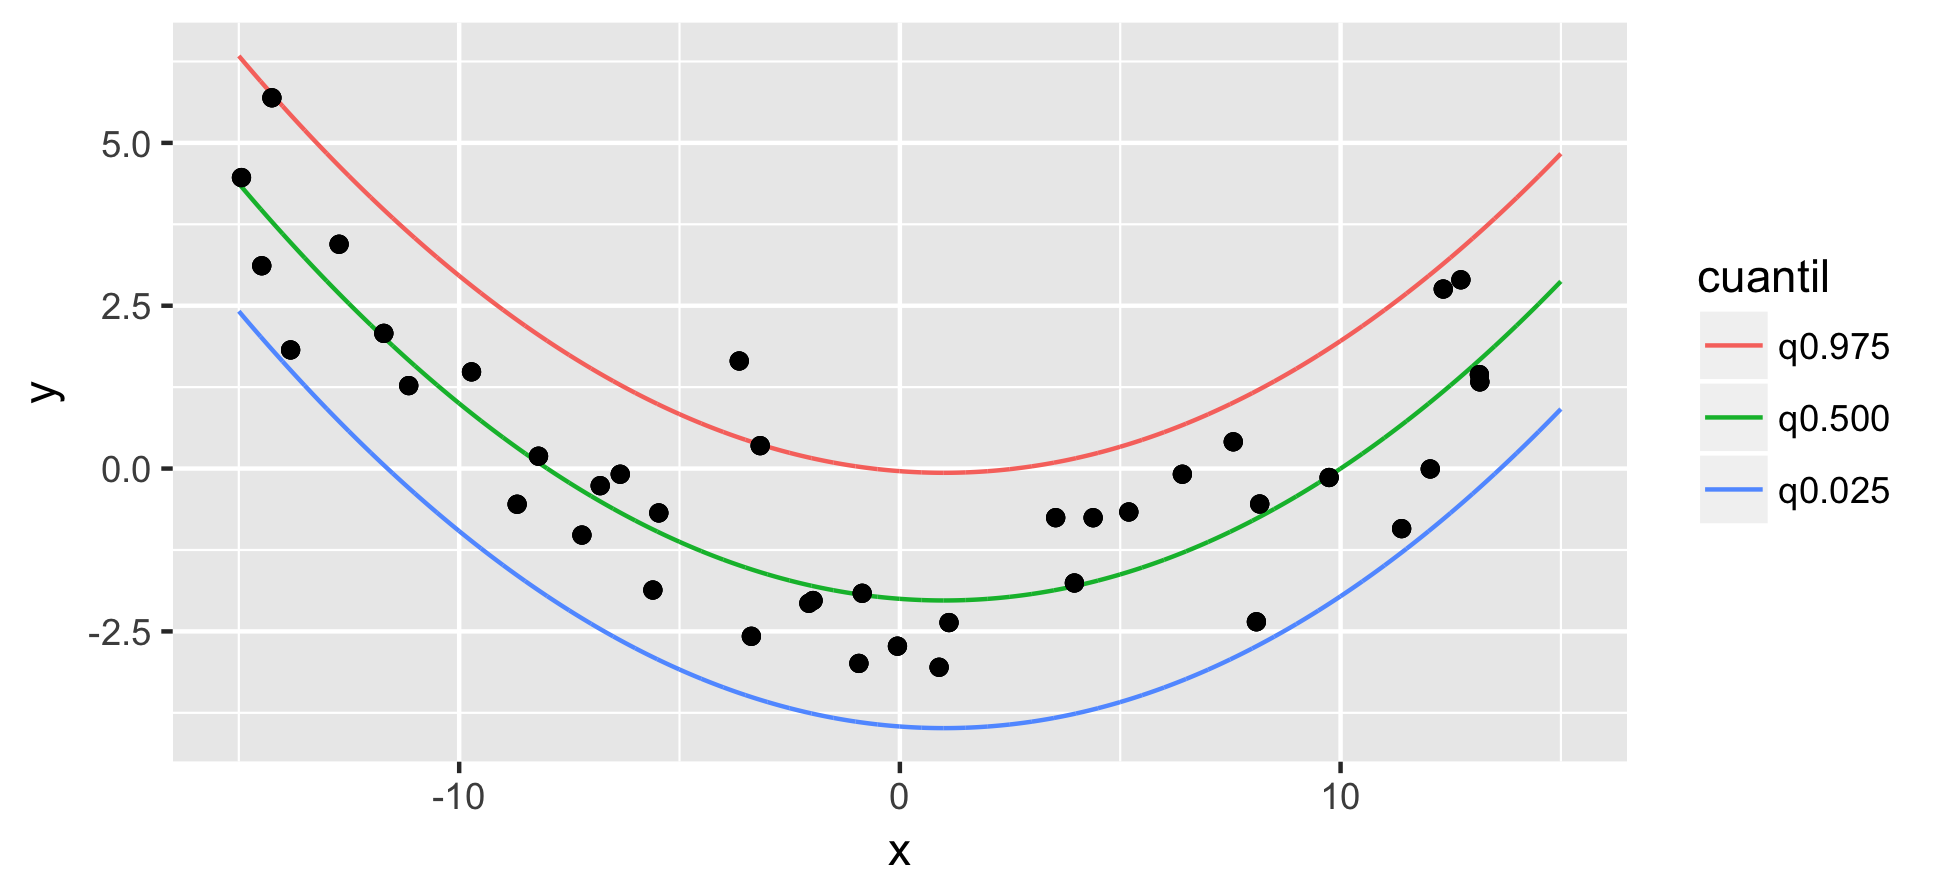
\includegraphics[width=0.60\textwidth]{Figures/Simulation/simple_g_simple_error/sample.png}
	\label{sample_sgse}
\end{figure}

\begin{figure}[H]
	\centering
	\caption{Ajuste del modelo \textit{GPDP}, para funci\'on simple y dispersi\'on simple.}
	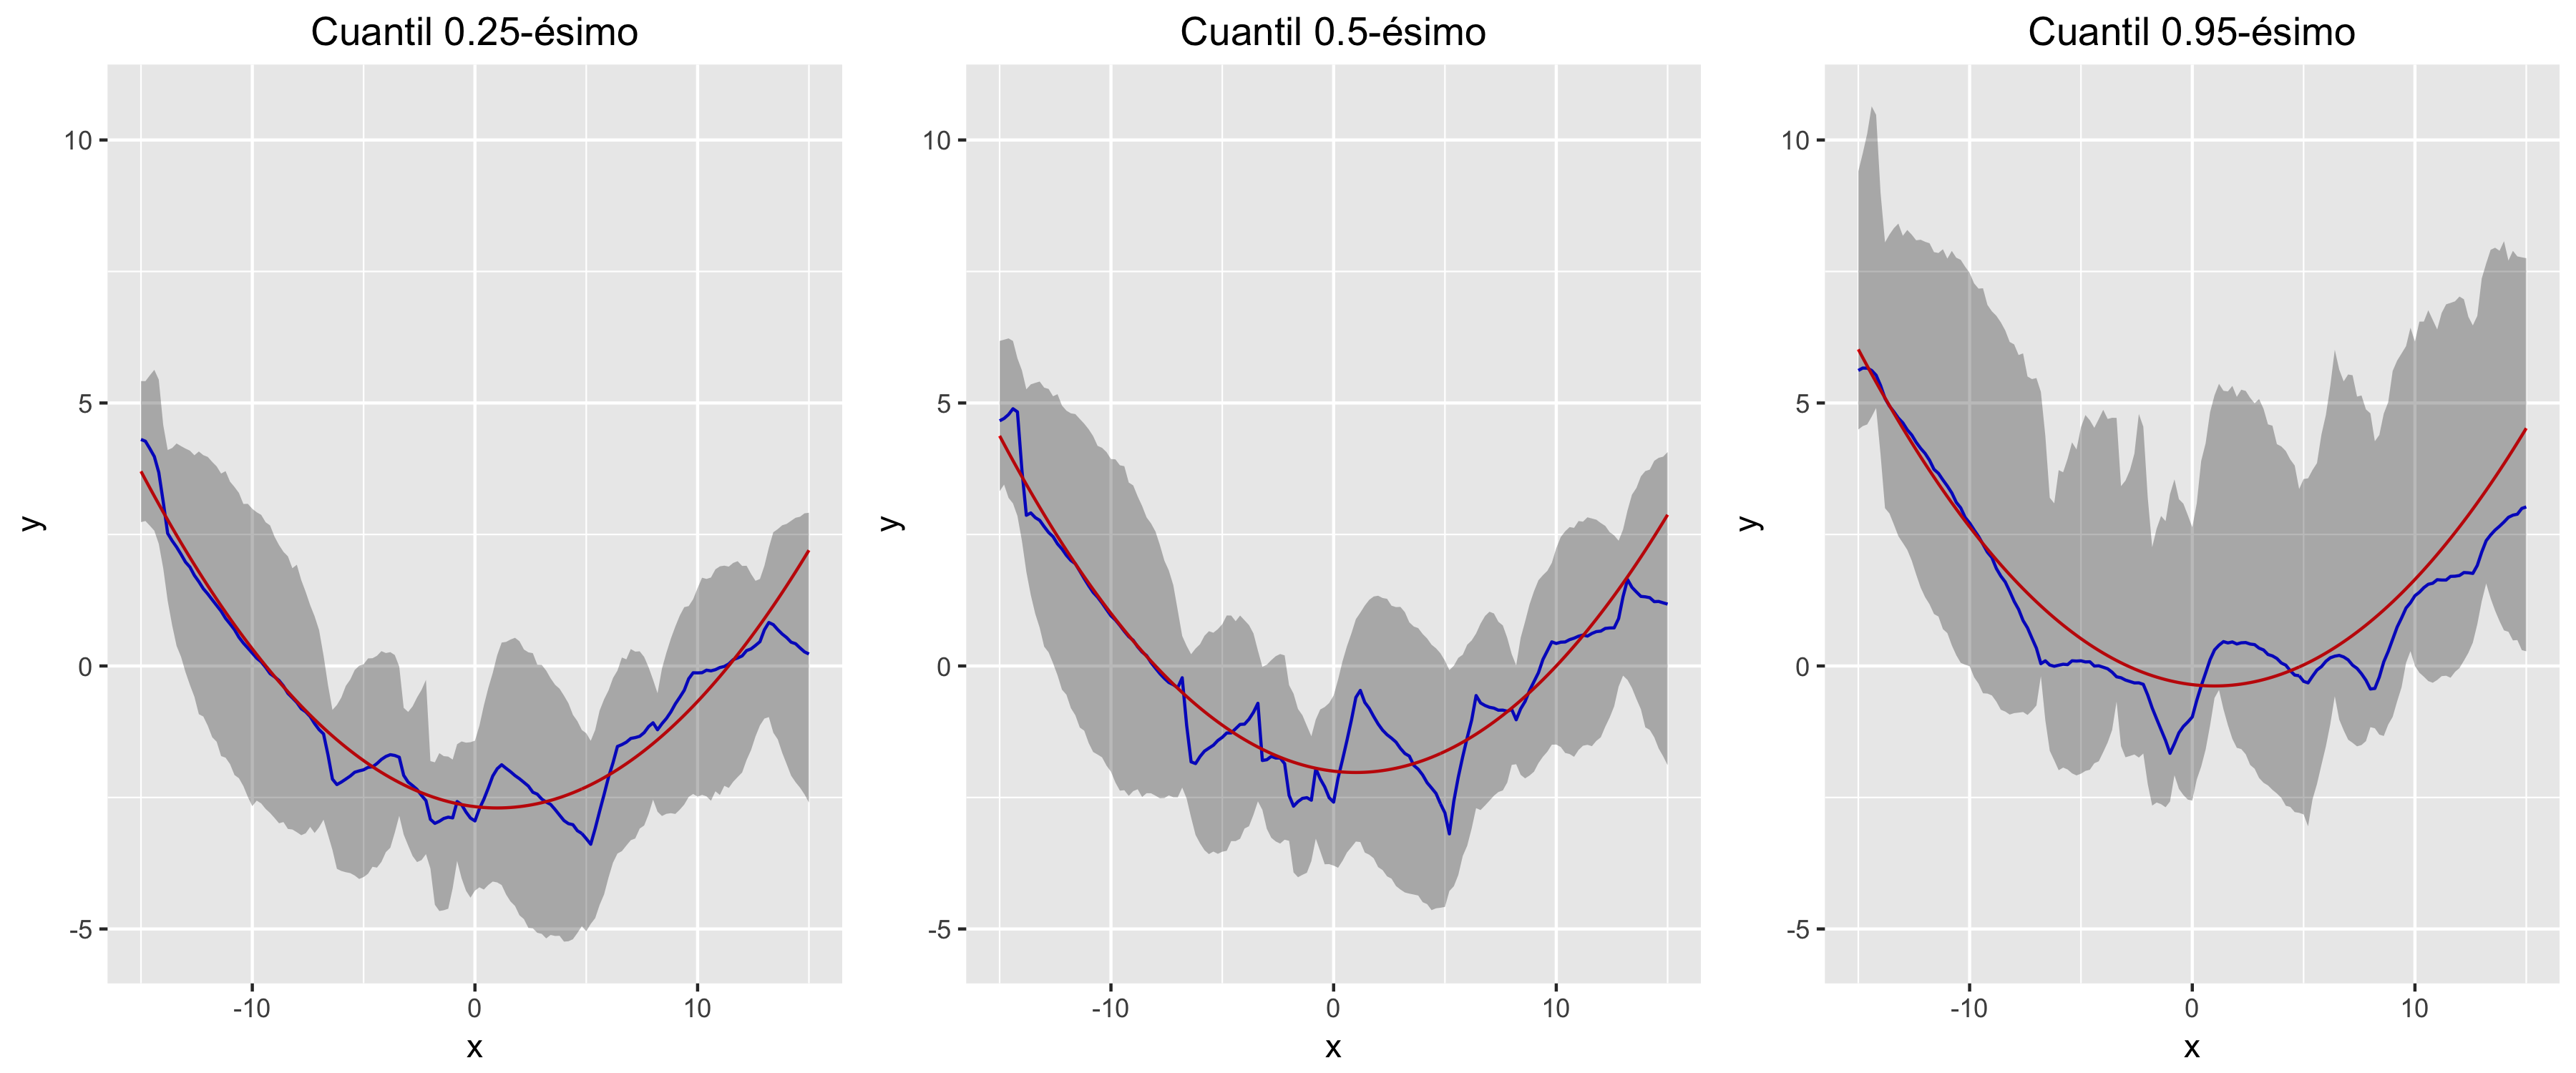
\includegraphics[width=\textwidth]{Figures/Simulation/simple_g_simple_error/fitted_models.png}
	\captionsetup{singlelinecheck=off,font=footnotesize}
    \caption*{Nota: La l\'inea roja representa el valor real de cada cuantil, la l\'inea azul representa la mediana de la distribuci\'on posterior predictiva y el \'area gris su intervalo de probabilidad al 90\%.}
	\label{fitted_sgse}
\end{figure}

Por otro lado, como se detall\'o en el cap\'itulo anterior, con el uso del paquete \textit{GPDPQuantReg} tambi\'en es posible algunos de los diagn\'osticos de las cadenas de Markov, los cuales se detallan en el \autoref{chap:MCMC}. Por ejemplo, se presentan los del cu\'antil $0.5$-\textit{\'esimo} en la figura \ref{diag_sgse}, mismos que reflejan un buen desempeño del algoritmo.

\begin{figure}[H]
	\centering
	\caption{Diagn\'osticos de las cadenas de Markov del cu\'antil $0.5$-\textit{\'esimo}, para funci\'on simple y dispersi\'on simple.}
	\subfloat[Ergodicidad]{
	    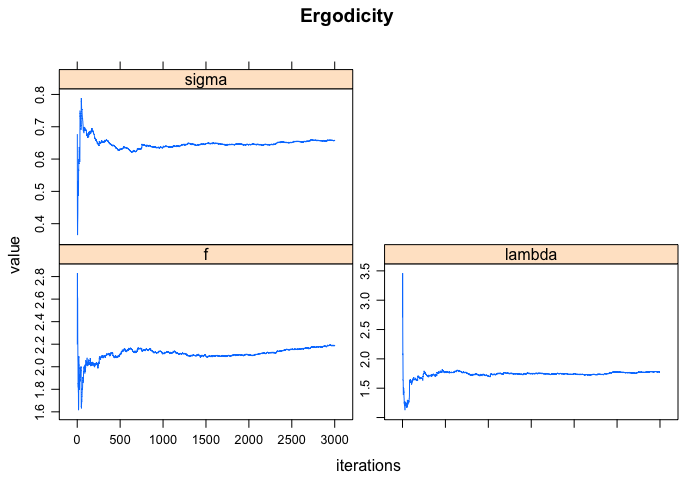
\includegraphics[width=0.45\textwidth]{Figures/Simulation/simple_g_simple_error/ergodicity.png}
	}
	\subfloat[Autocorrelaci\'on]{
	    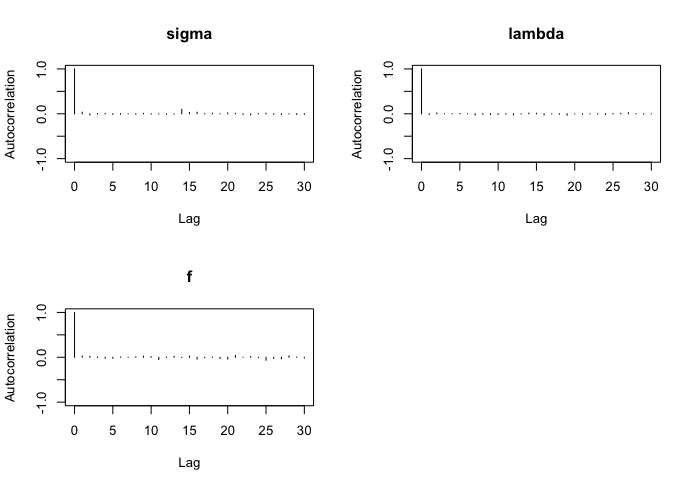
\includegraphics[width=0.45\textwidth]{Figures/Simulation/simple_g_simple_error/autocorrelation.png}
	}\\
	\subfloat[Correlaci\'on cruzada]{
	    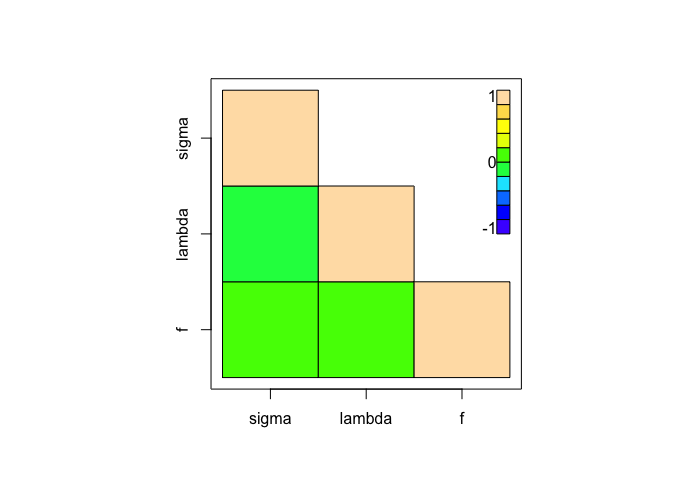
\includegraphics[width=0.45\textwidth]{Figures/Simulation/simple_g_simple_error/crosscorrelation.png}
	}
	\subfloat[Traza]{
	    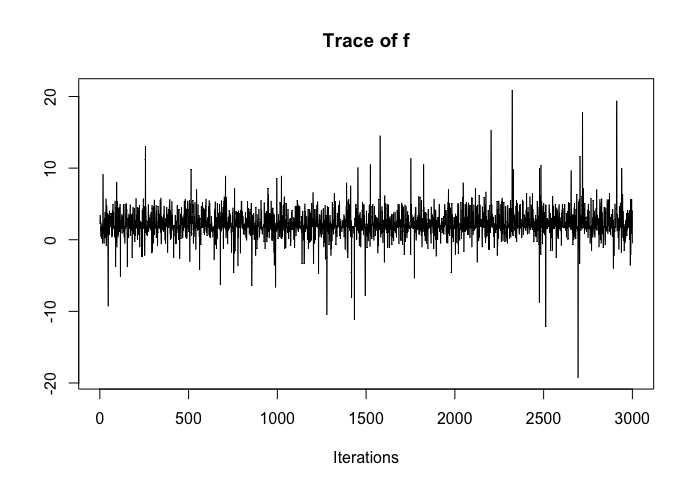
\includegraphics[width=0.45\textwidth]{Figures/Simulation/simple_g_simple_error/trace.png}
	}
	\label{diag_sgse}
\end{figure}

\subsection{Funci\'on compleja, dispersi\'on simple}

En este caso, se mantuvo que $E \sim \mathcal{N}(1,0)$, pero la funci\'on $g$ usada fue m\'as compleja:
\begin{equation*}
    g(x) = \frac{1}{2} x \cos(x) - \exp\left(\frac{1}{10}x\right).
\end{equation*}

Los datos simulados se pueden observar en la figura \ref{sample_cgse}, los cuales al ajustar el modelo mostraron de nuevo buenos resultados (figura \ref{fitted_cgse}), apareciendo la funci\'on original adentro del intervalo de probabilidad al 90\% en pr\'acticamente todos los valores de $x$ en los que se realiz\'o predicci\'on, a excepci\'on de la \'ultima zona, en la que no hubo datos de entrenamiento.

\begin{figure}[H]
	\centering
	\caption{Datos simulados y cuantiles de referencia, para funci\'on compleja y dispersi\'on simple.}
	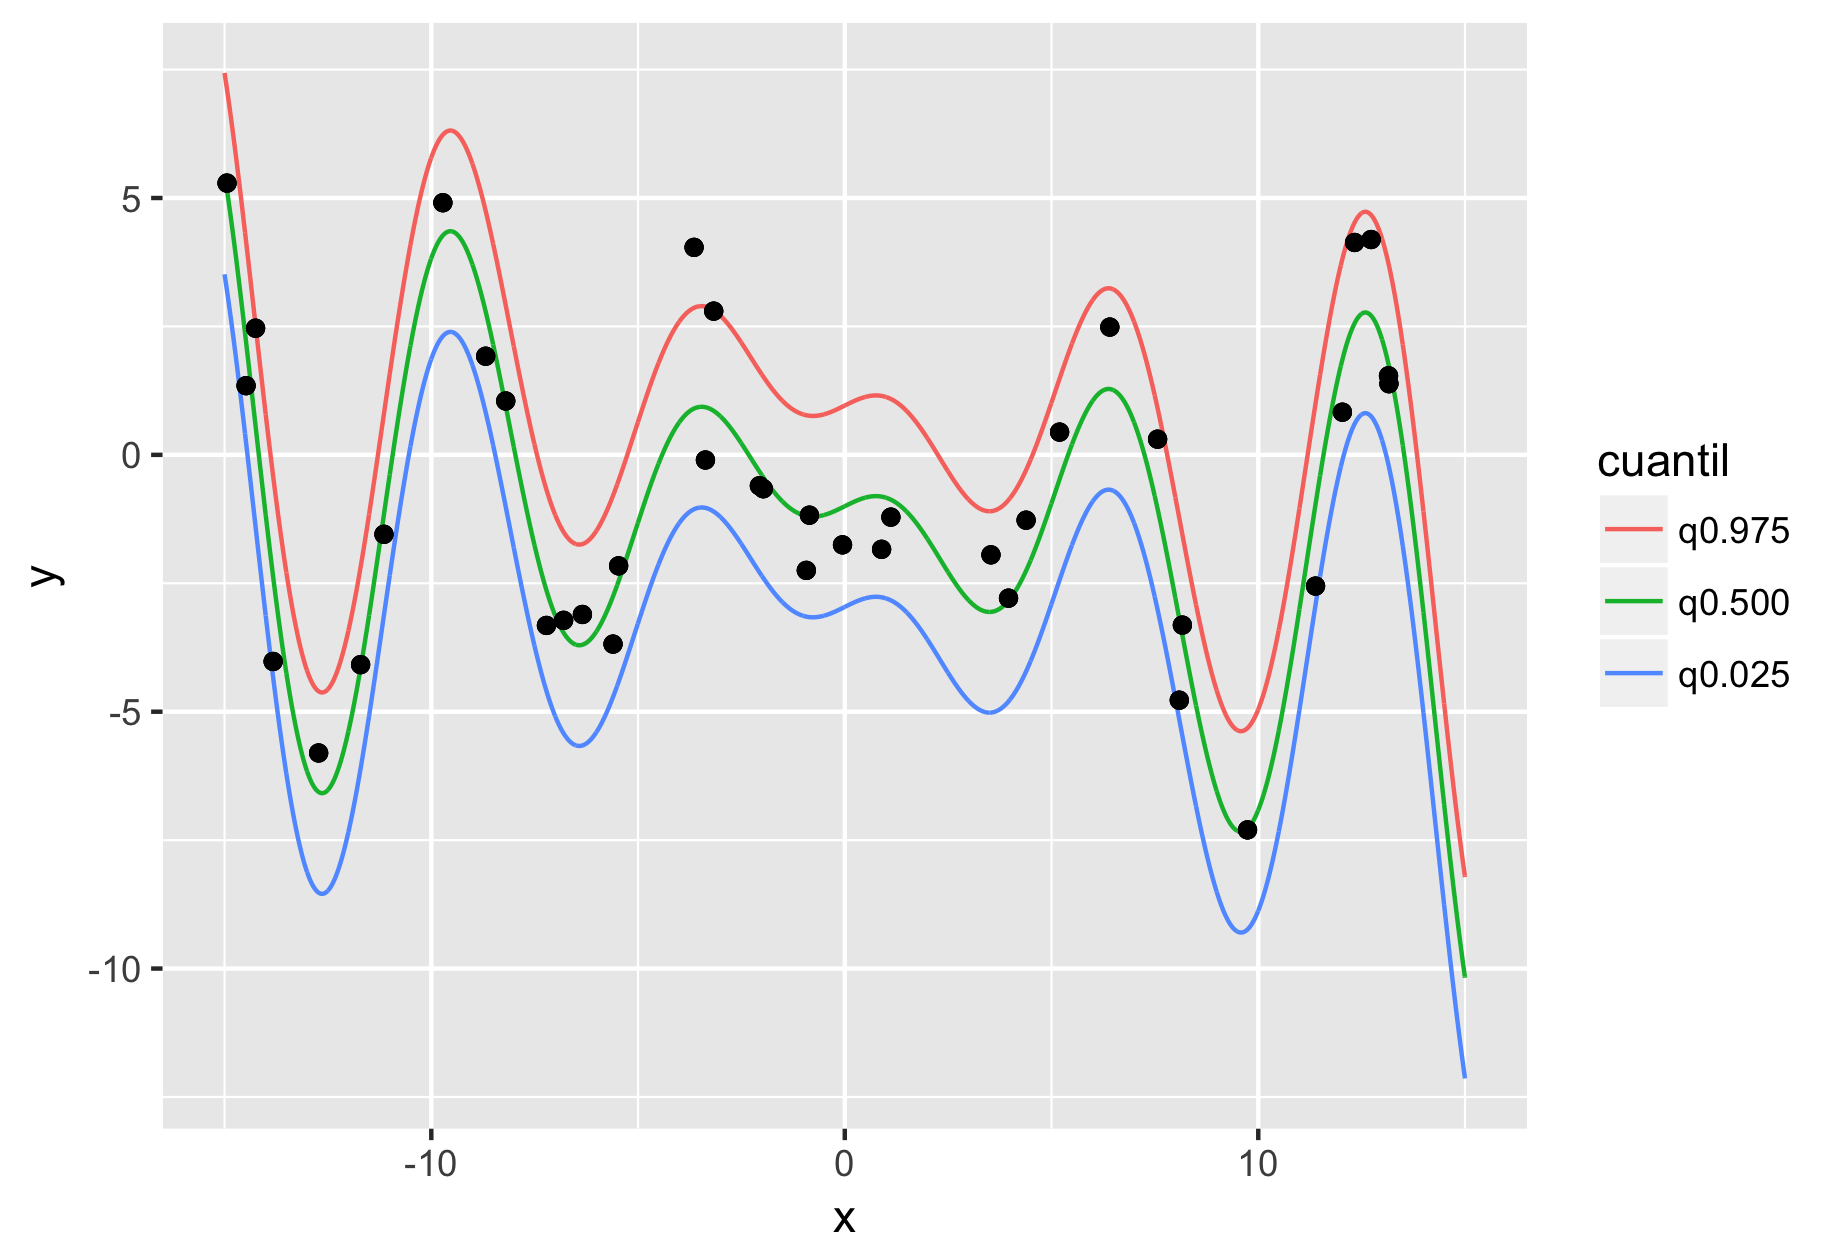
\includegraphics[width=0.60\textwidth]{Figures/Simulation/complex_g_simple_error/sample.png}
	\label{sample_cgse}
\end{figure}

\begin{figure}[H]
	\centering
	\caption{Ajuste del modelo \textit{GPDP}, para funci\'on compleja y dispersi\'on simple.}
	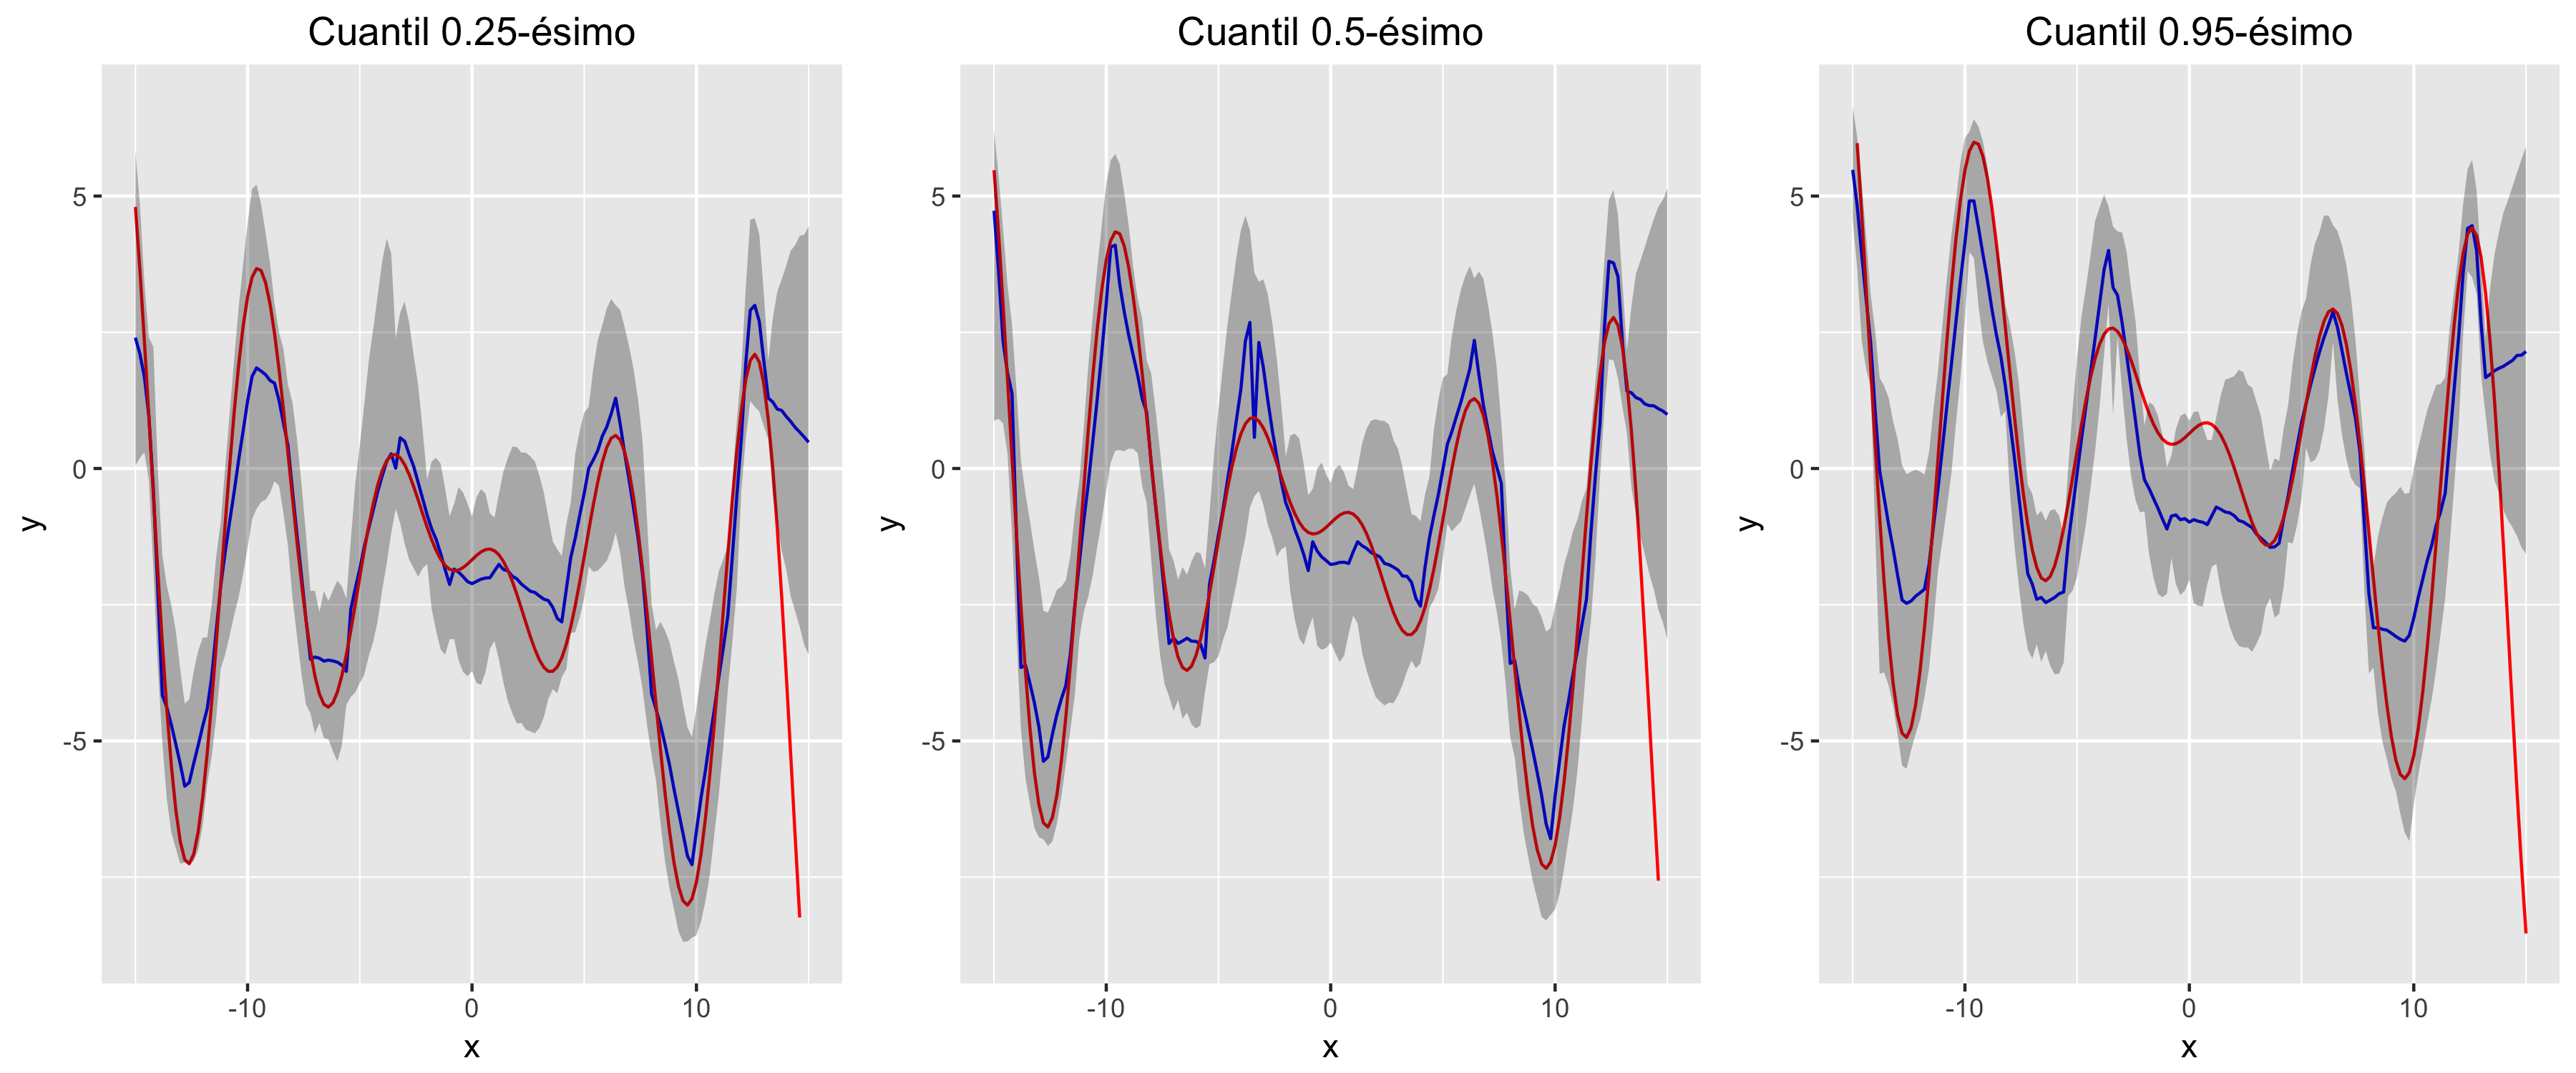
\includegraphics[width=\textwidth]{Figures/Simulation/complex_g_simple_error/fitted_models.png}
	\captionsetup{singlelinecheck=off, font=footnotesize}
    \caption*{Nota: La l\'inea roja representa el valor real de cada cuantil, la l\'inea azul representa la mediana de la distribuci\'on posterior predictiva y el \'area gris su intervalo de probabilidad al 90\%.}
	\label{fitted_cgse}
\end{figure}

\subsection{Funci\'on simple, dispersi\'on compleja}

En este caso, se uso una funci\'on lineal $g$:
\begin{equation*}
    g(x) = \frac{1}{2} x.
\end{equation*}
La complejidad se introdujo en $E \sim \textit{Gamma}(\alpha = 2,\beta = 1)$, debido a que la dipersi\'on no fue sim\'etrica y fue acotada por la izquierda. 

El conjunto de datos usado para este modelo aparece en la figura \ref{sample_sgce}, y a pesar de la complejidad de la dispersi\'on, se obtuvieron buenos resultados (figura \ref{fitted_sgce}), debido a que nuevamente las funciones reales de los diversos cuantiles cayeron en su totalidad dentro del intervalo de probabilidad al 90\%, estimado por el modelo.

Un detalle notable es que, al igual que el caso de funci\'on simple y dispersi\'on simple, la estimaci\'on de la funci\'on del cuantil 0.95\textit{-\'esimo} muestra una varianza m\'as grande que los otros dos cuantiles. Esto debido a que en valores extremos el modelo refleja mayor incertidumbre de lo que en realidad podr\'ia estar ocurriendo.

\begin{figure}[H]
	\centering
	\caption{Datos simulados y cuantiles de referencia, para funci\'on simple y dispersi\'on compleja.}
	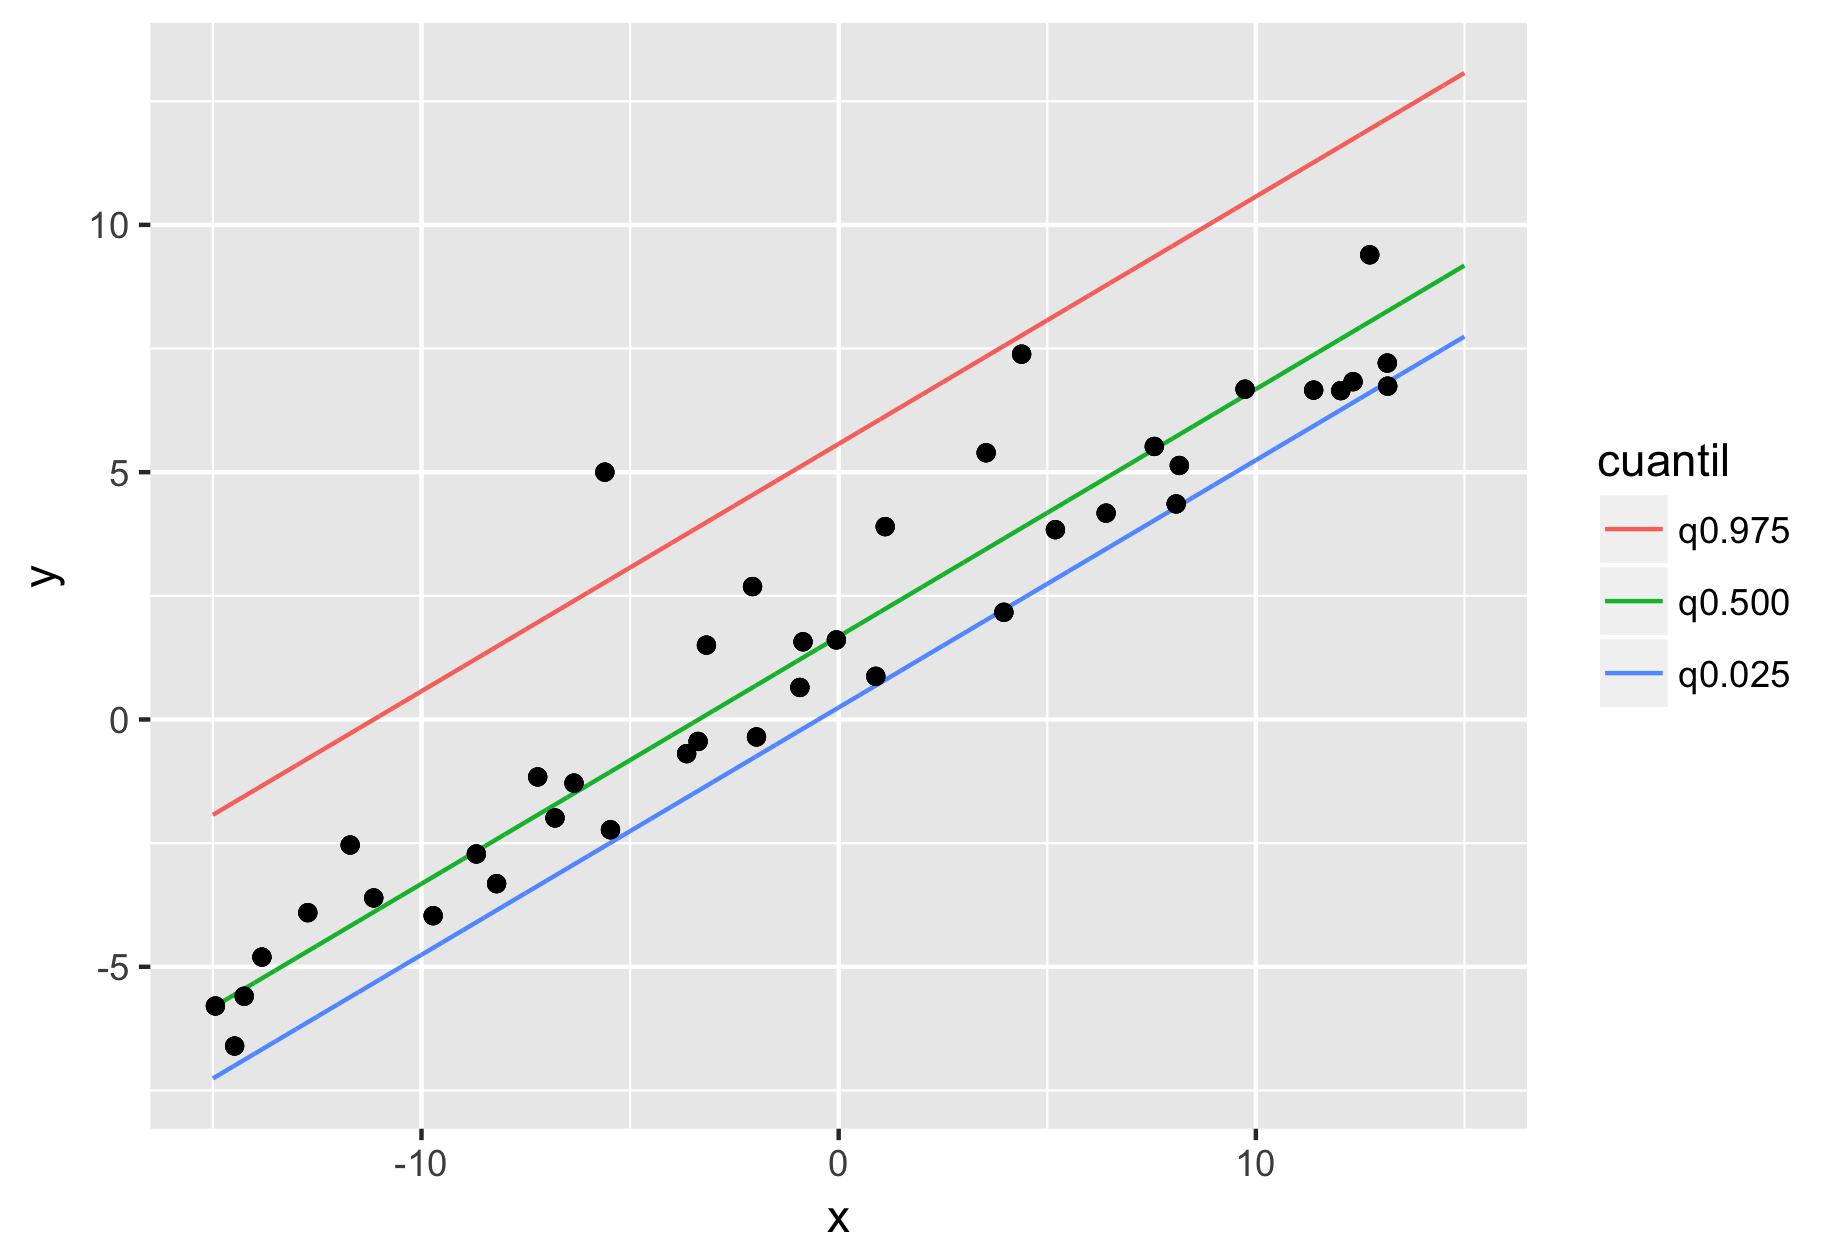
\includegraphics[width=0.60\textwidth]{Figures/Simulation/simple_g_complex_error/sample.png}
	\label{sample_sgce}
\end{figure}

\begin{figure}[H]
	\centering
	\caption{Ajuste del modelo \textit{GPDP}, para funci\'on simple y dispersi\'on compleja.}
	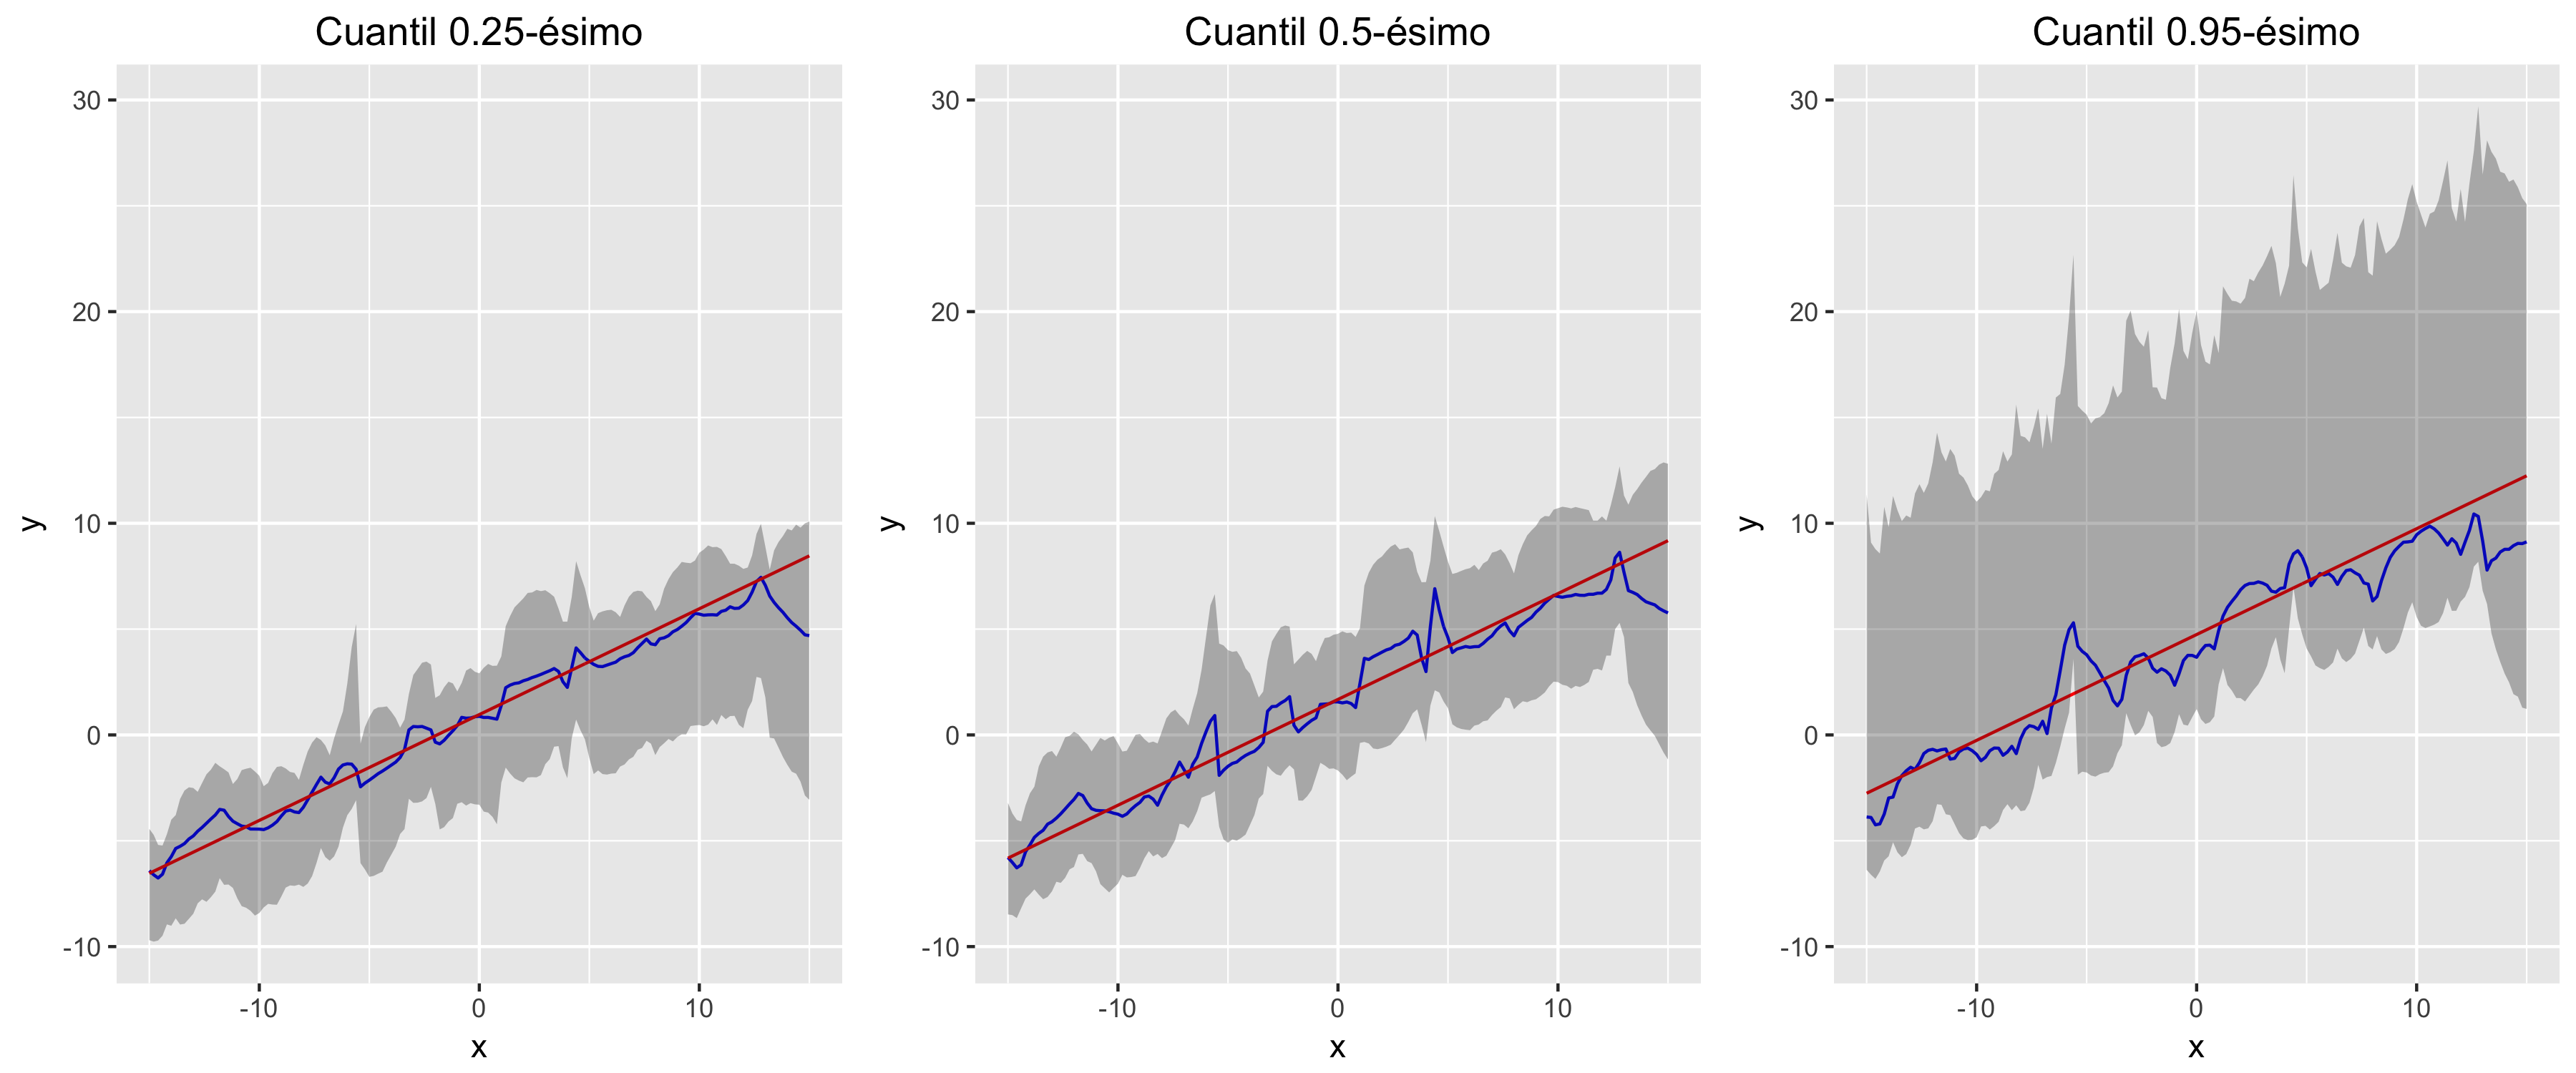
\includegraphics[width=\textwidth]{Figures/Simulation/simple_g_complex_error/fitted_models.png}
	\captionsetup{singlelinecheck=off,font=footnotesize}
    \caption*{Nota: La l\'inea roja representa el valor real de cada cuantil, la l\'inea azul representa la mediana de la distribuci\'on posterior predictiva y el \'area gris su intervalo de probabilidad al 90\%.}
	\label{fitted_sgce}
\end{figure}

\subsection{Funci\'on compleja, dispersi\'on compleja}

En este modelo se usaron datos (figura \ref{sample_cgce}) provenientes tanto de una dispersi\'on compleja, $E \sim \textit{Gamma}(\alpha = 2,\beta = 1)$, como de una funci\'on $g$ compleja:
\begin{equation*}
    g(x) = \frac{1}{2} x \cos(x) - \exp\left(\frac{1}{10}x\right).
\end{equation*}

Despu\'es del ajuste (figura \ref{fitted_cgce}), el balance fue positivo, debido a que las funciones reales de los diversos cuantiles cayeron en su totalidad dentro del intervalo de probabilidad al 90\%, del estimado por el modelo, a excepci\'
on de la zona de la que no se tuvieron datos, como en el caso de funci\'on compleja y dispersi\'on simple. Pero a diferencia de ese modelo, la dispersi\'on compleja produce una mayor incertidumbre, particularmente notoria en el caso del cuantil 0.95\textit{-\'esimo}.

\begin{figure}[H]
	\centering
	\caption{Datos simulados y cuantiles de referencia, para funci\'on compleja y dispersi\'on compleja.}
	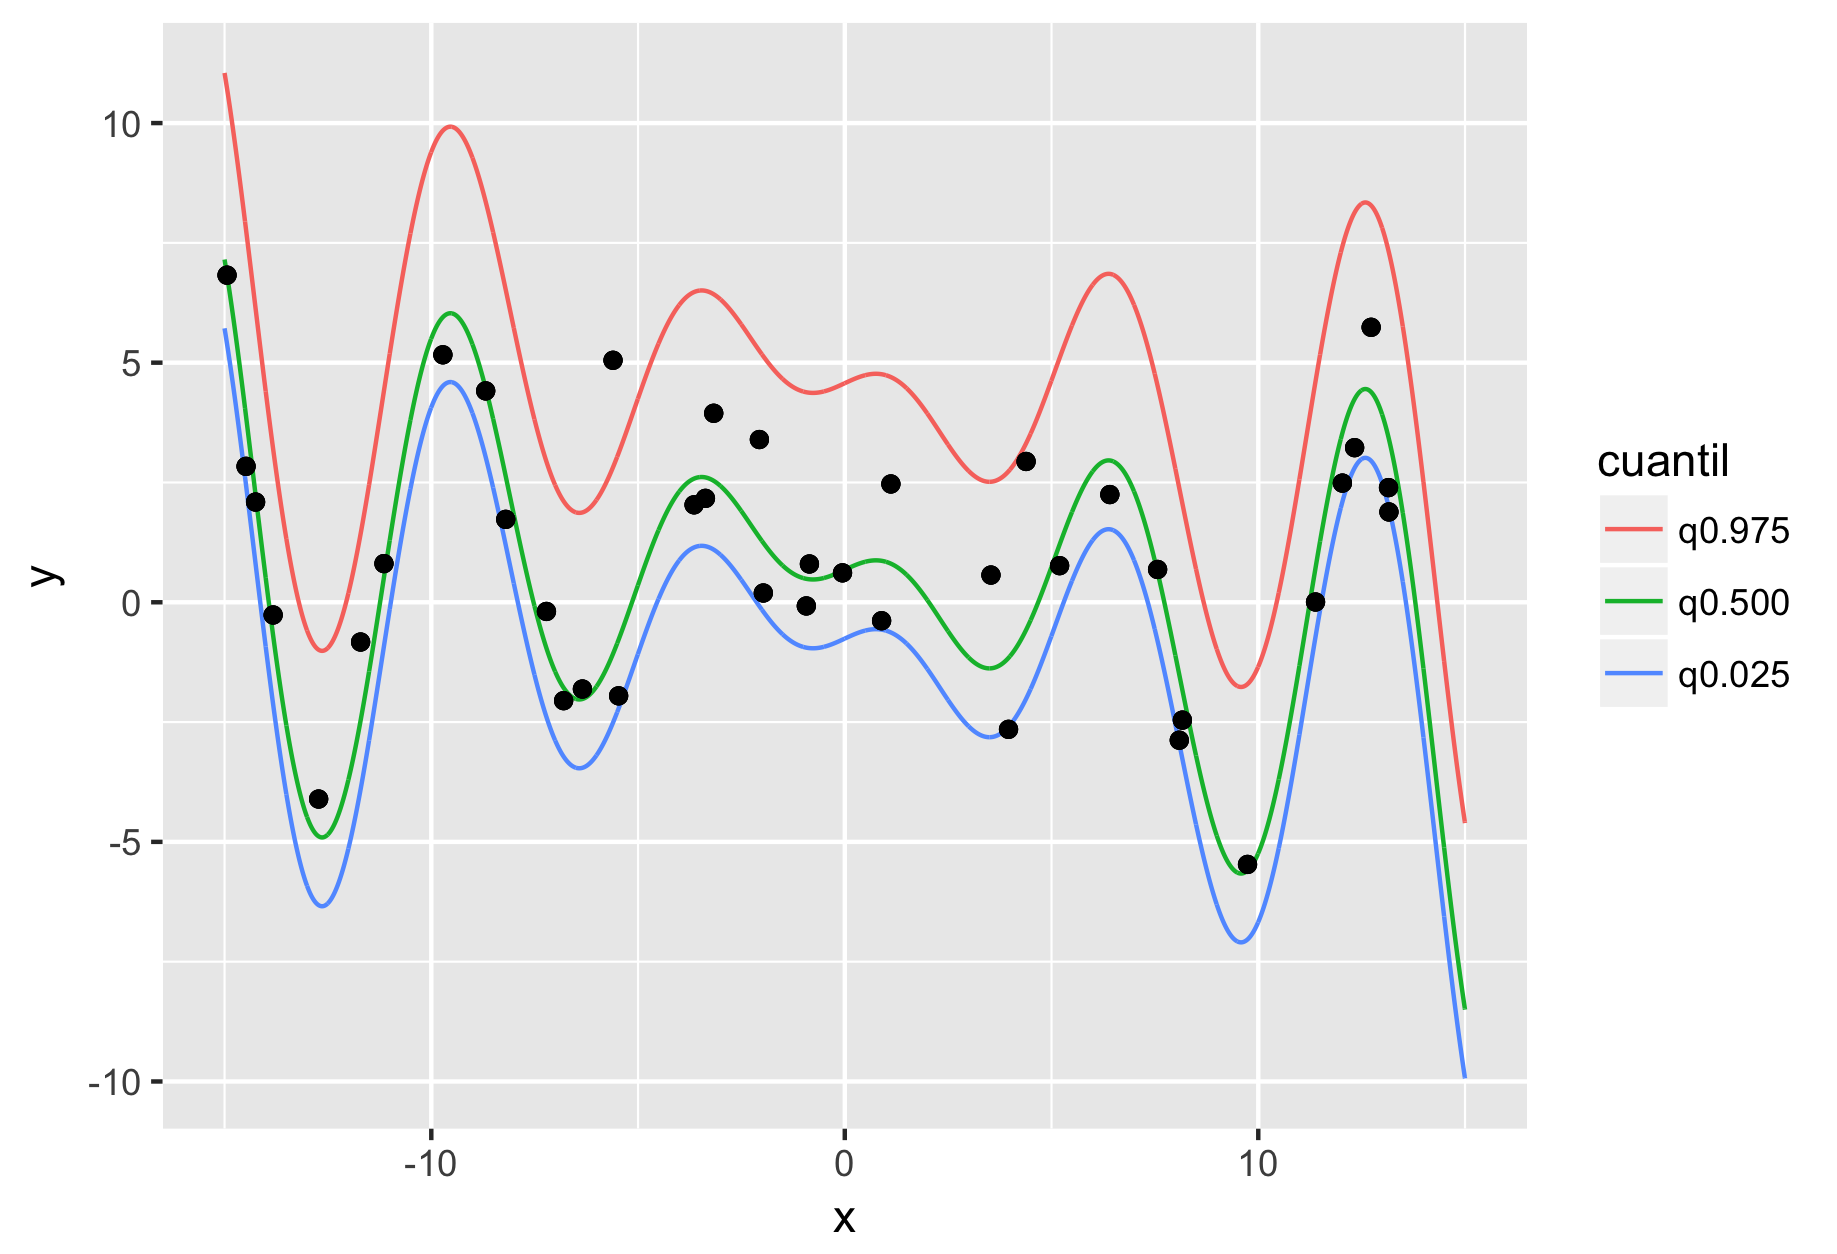
\includegraphics[width=0.60\textwidth]{Figures/Simulation/complex_g_complex_error/sample.png}
	\label{sample_cgce}
\end{figure}

\begin{figure}[H]
	\centering
	\caption{Ajuste del modelo \textit{GPDP}, para funci\'on compleja y dispersi\'on compleja.}
	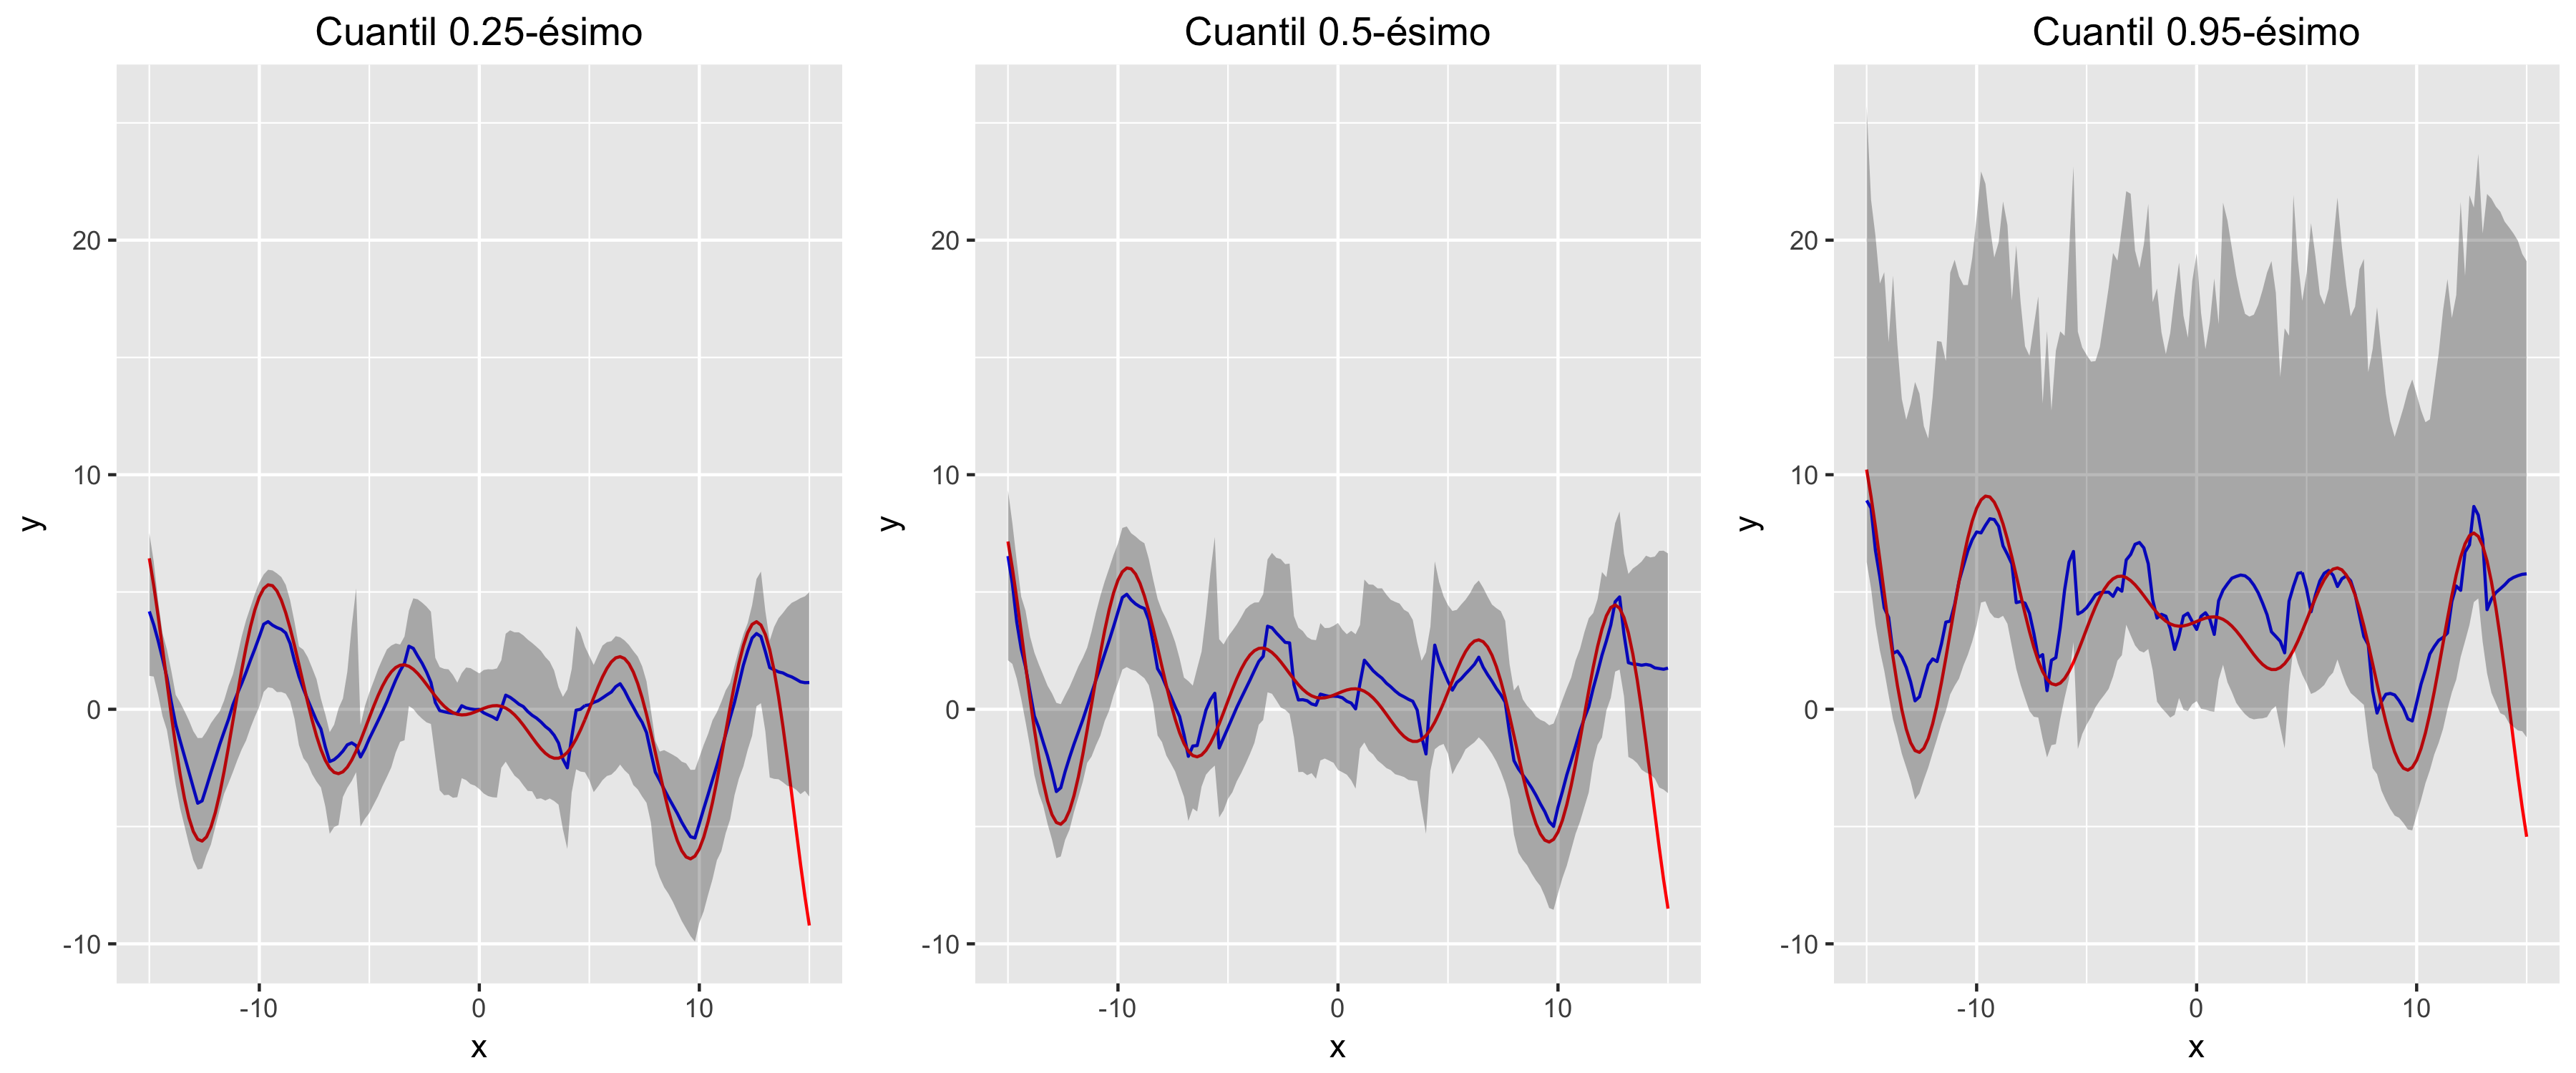
\includegraphics[width=\textwidth]{Figures/Simulation/complex_g_complex_error/fitted_models.png}
	\captionsetup{singlelinecheck=off,font=footnotesize}
    \caption*{Nota: La l\'inea roja representa el valor real de cada cuantil, la l\'inea azul representa la mediana de la distribuci\'on posterior predictiva y el \'area gris su intervalo de probabilidad al 90\%.}
	\label{fitted_cgce}
\end{figure}

\section{Investigaci\'on de mercados}

\subsection{Conceptos iniciales}

En el contexto de la investigaci\'on de mercados una de las m\'etricas que se consideran m\'as importantes es la del \textit{Conocimiento de marca}, misma que se define como el porcentaje de una cierta poblaci\'on que declara conocer el nombre de la marca en cuesti\'on.

Dentro de dicho ambiente, la teor\'ia dice que esa m\'etrica normalmente depende de la publicidad pautada semana a semana. Cuando una marca \'unicamente se publicita en televisi\'on, el valor com\'unmente usado para medir esa inversi\'on se denomina \textit{Adstocked GRP}s, y, en esencia, se compone de cu\'antas veces se transmiti\'o el comercial y cu\'anta gente estaba viendo la televisi\'on cuando se transmiti\'o,  ponderado por qu\'e tan lejana en el tiempo fue dicha transmisi\'on, respecto al d\'ia de hoy. Asimismo, tambi\'en se suelen usar las inversiones de los competidores para explicar el \textit{Conocimiento de marca}, debido a que es com\'un que las personas se confundan y asocien a la marca un comercial del competidor.

En el pasado, inversiones iguales han representado resultados ligeramente distintos en los niveles de \textit{Conocimiento de marca}, situaci\'on que normalmente es asociada a la calidad de los comerciales, tanto los propios, como los del competidor. En otras palabras, comerciales m\'as memorables han generado un mayor \textit{Conocimiento de marca} a la que los pauta, y una aportaci\'on muy pequeña al competidor, cuando se han transmitido en aproximadamente la misma cantidad ocasiones y a una similar audiencia.

Adem\'as, tambi\'en es importante revisar el concepto de \textit{marca madre} y \textit{subvariantes}, para nuestra siguiente aplicaci\'on del modelo GPDP. Una \textit{marca madre} es aquella que tiene fama por su propio nombre, pero que se ofrece al consumidor mediante productos (tambi\'en llamados \textit{subvariantes}) que son publicitados por s\'i solos. Por ejemplo, se puede pensar en la empresa de tecnolog\'ia \textit{Pera} que tiene comerciales que posicionan su nombre, pero tiene tambi\'en comerciales donde promociona \'unicamente el celular que producen, y en otros, \'unicamente la tableta.

Dicho esto, normalmente se piensa que los comerciales de la \textit{marca madre} contribuyen m\'as al \textit{Conocimiento de marca} que aquellos de las \textit{subvariantes}, que tienen como prop\'osito vender los productos espec\'ificos, m\'as que posicionar la marca.

\subsection{Caso real}

Cierta \textit{marca madre} es cliente de la empresa de investigaci\'on de mercados en la que sol\'ia trabajar. Dicha marca registr\'o semana a semana los valores de inversi\'on en sus comerciales, la realizada para los de sus \textit{subvariantes}, la de su competencia y el \textit{Conocimiento de marca} reportado durante 2014 y 2015. Estos sirvieron para entrenar un modelo GPDP, bajo el supuesto que las mediciones semanales fueron independientes. Los valores predichos comparados contra los que en efecto se observaron se presentan a continuaci\'on.

\begin{figure}[H]
	\centering
	\caption{Modelo de \textit{Conocimiento de marca} para datos de entrenamiento (2014-2015).}
	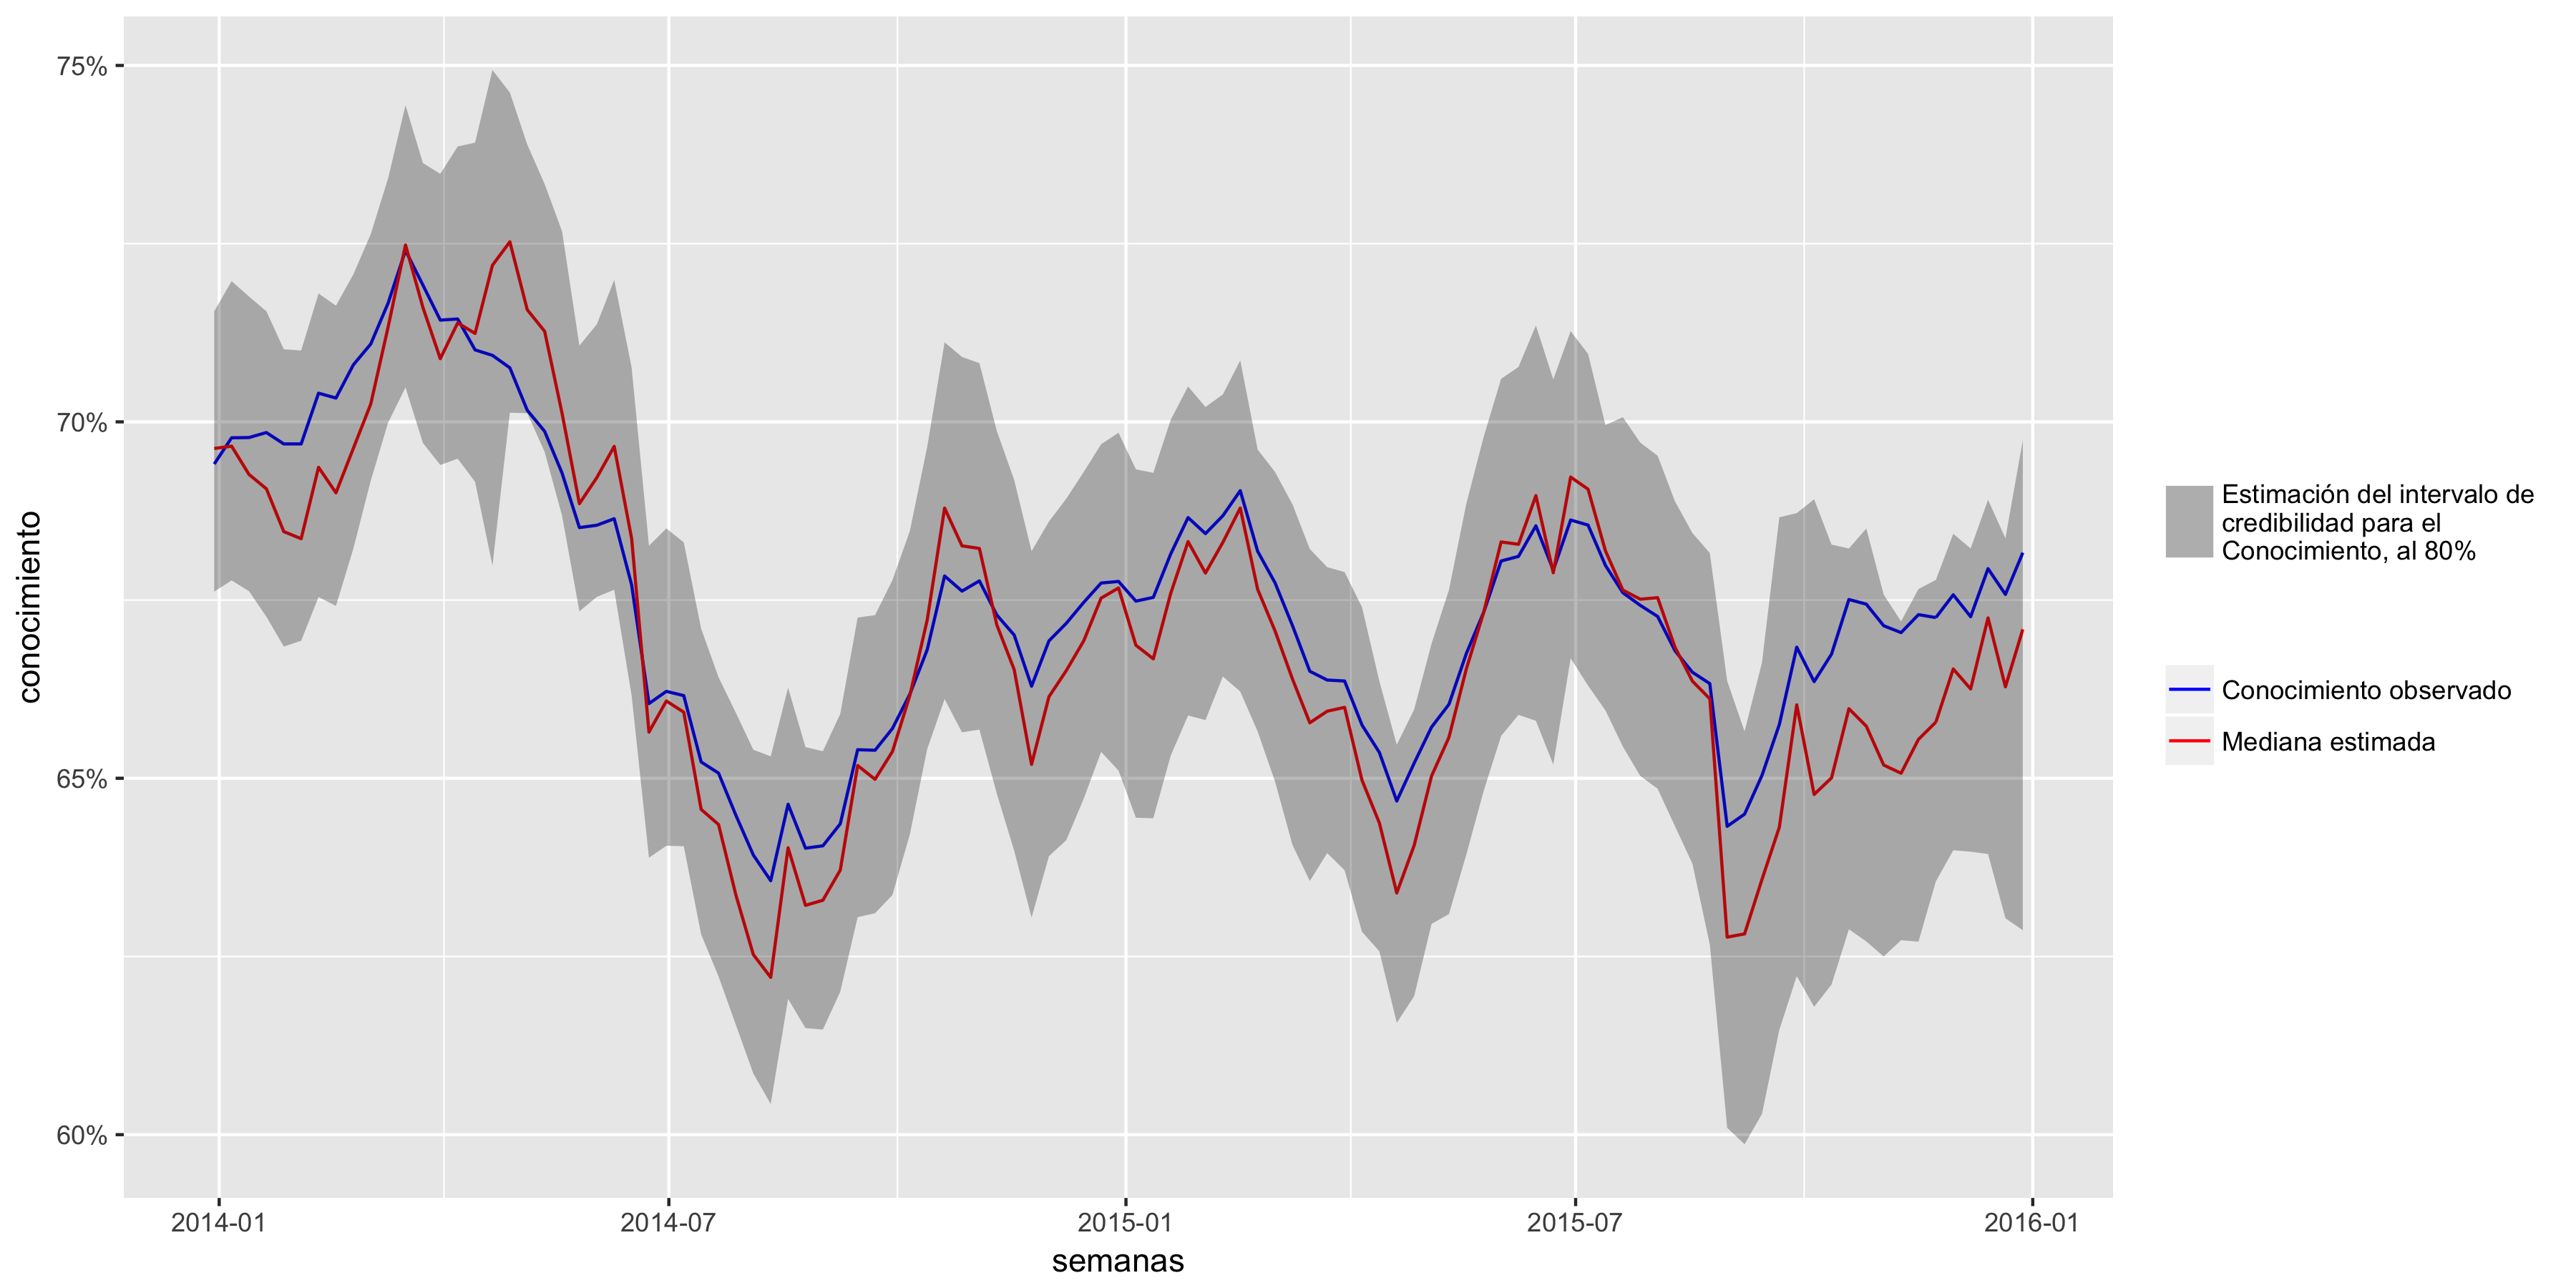
\includegraphics[width=1\textwidth]{Figures/MarketResearch/fit_review.png}
	\captionsetup{singlelinecheck=off,font=footnotesize}
	\caption*{Nota: El intervalo de credibilidad se construy\'o usando las estimaciones de la mediana de los cuantiles $0.05$-\'esimo y $0.95$-\'esimo.}
	\label{awareness_fit}
\end{figure}

Como se puede observar, el \textit{Conocimiento de marca} sigue un movimiento muy similar a la mediana que predijo el modelo, y, de hecho, en los \'ultimos meses se ha despegado positivamente.

Todo esto se hizo ignorando el hecho de que tambi\'en se ten\'ian los datos de 2016, para ver c\'omo funcionar\'ia el modelo. Al cliente particularmente le interesaba ver esto porque la m\'etrica tuvo una estrepitosa ca\'ida durante el 2016 y ten\'ia la duda si era por una estrategia desafortunada de su inversi\'on o por el hecho de que su competidor hab\'ia cambiado completamente el concepto de sus comerciales, situaci\'on que podr\'ia estar provocando que la gente ya no se confundiera y los relacionara err\'oneamente a los de nuestro cliente.

Traslado al lenguaje del modelo, se deseaba ver si el valor realmente observado pudo haber sido predicho por el modelo o si lo consideraba poco probable, situaci\'on en la que efectivamente se podr\'ia hablar de un cambio estructural ocurrido dentro de este contexto. Los resultados obtenidos fueron los siguientes.

\begin{figure}[H]
	\centering
	\caption{\textit{Conocimiento de marca} en 2016, comparado con el modelo GPDP.}
	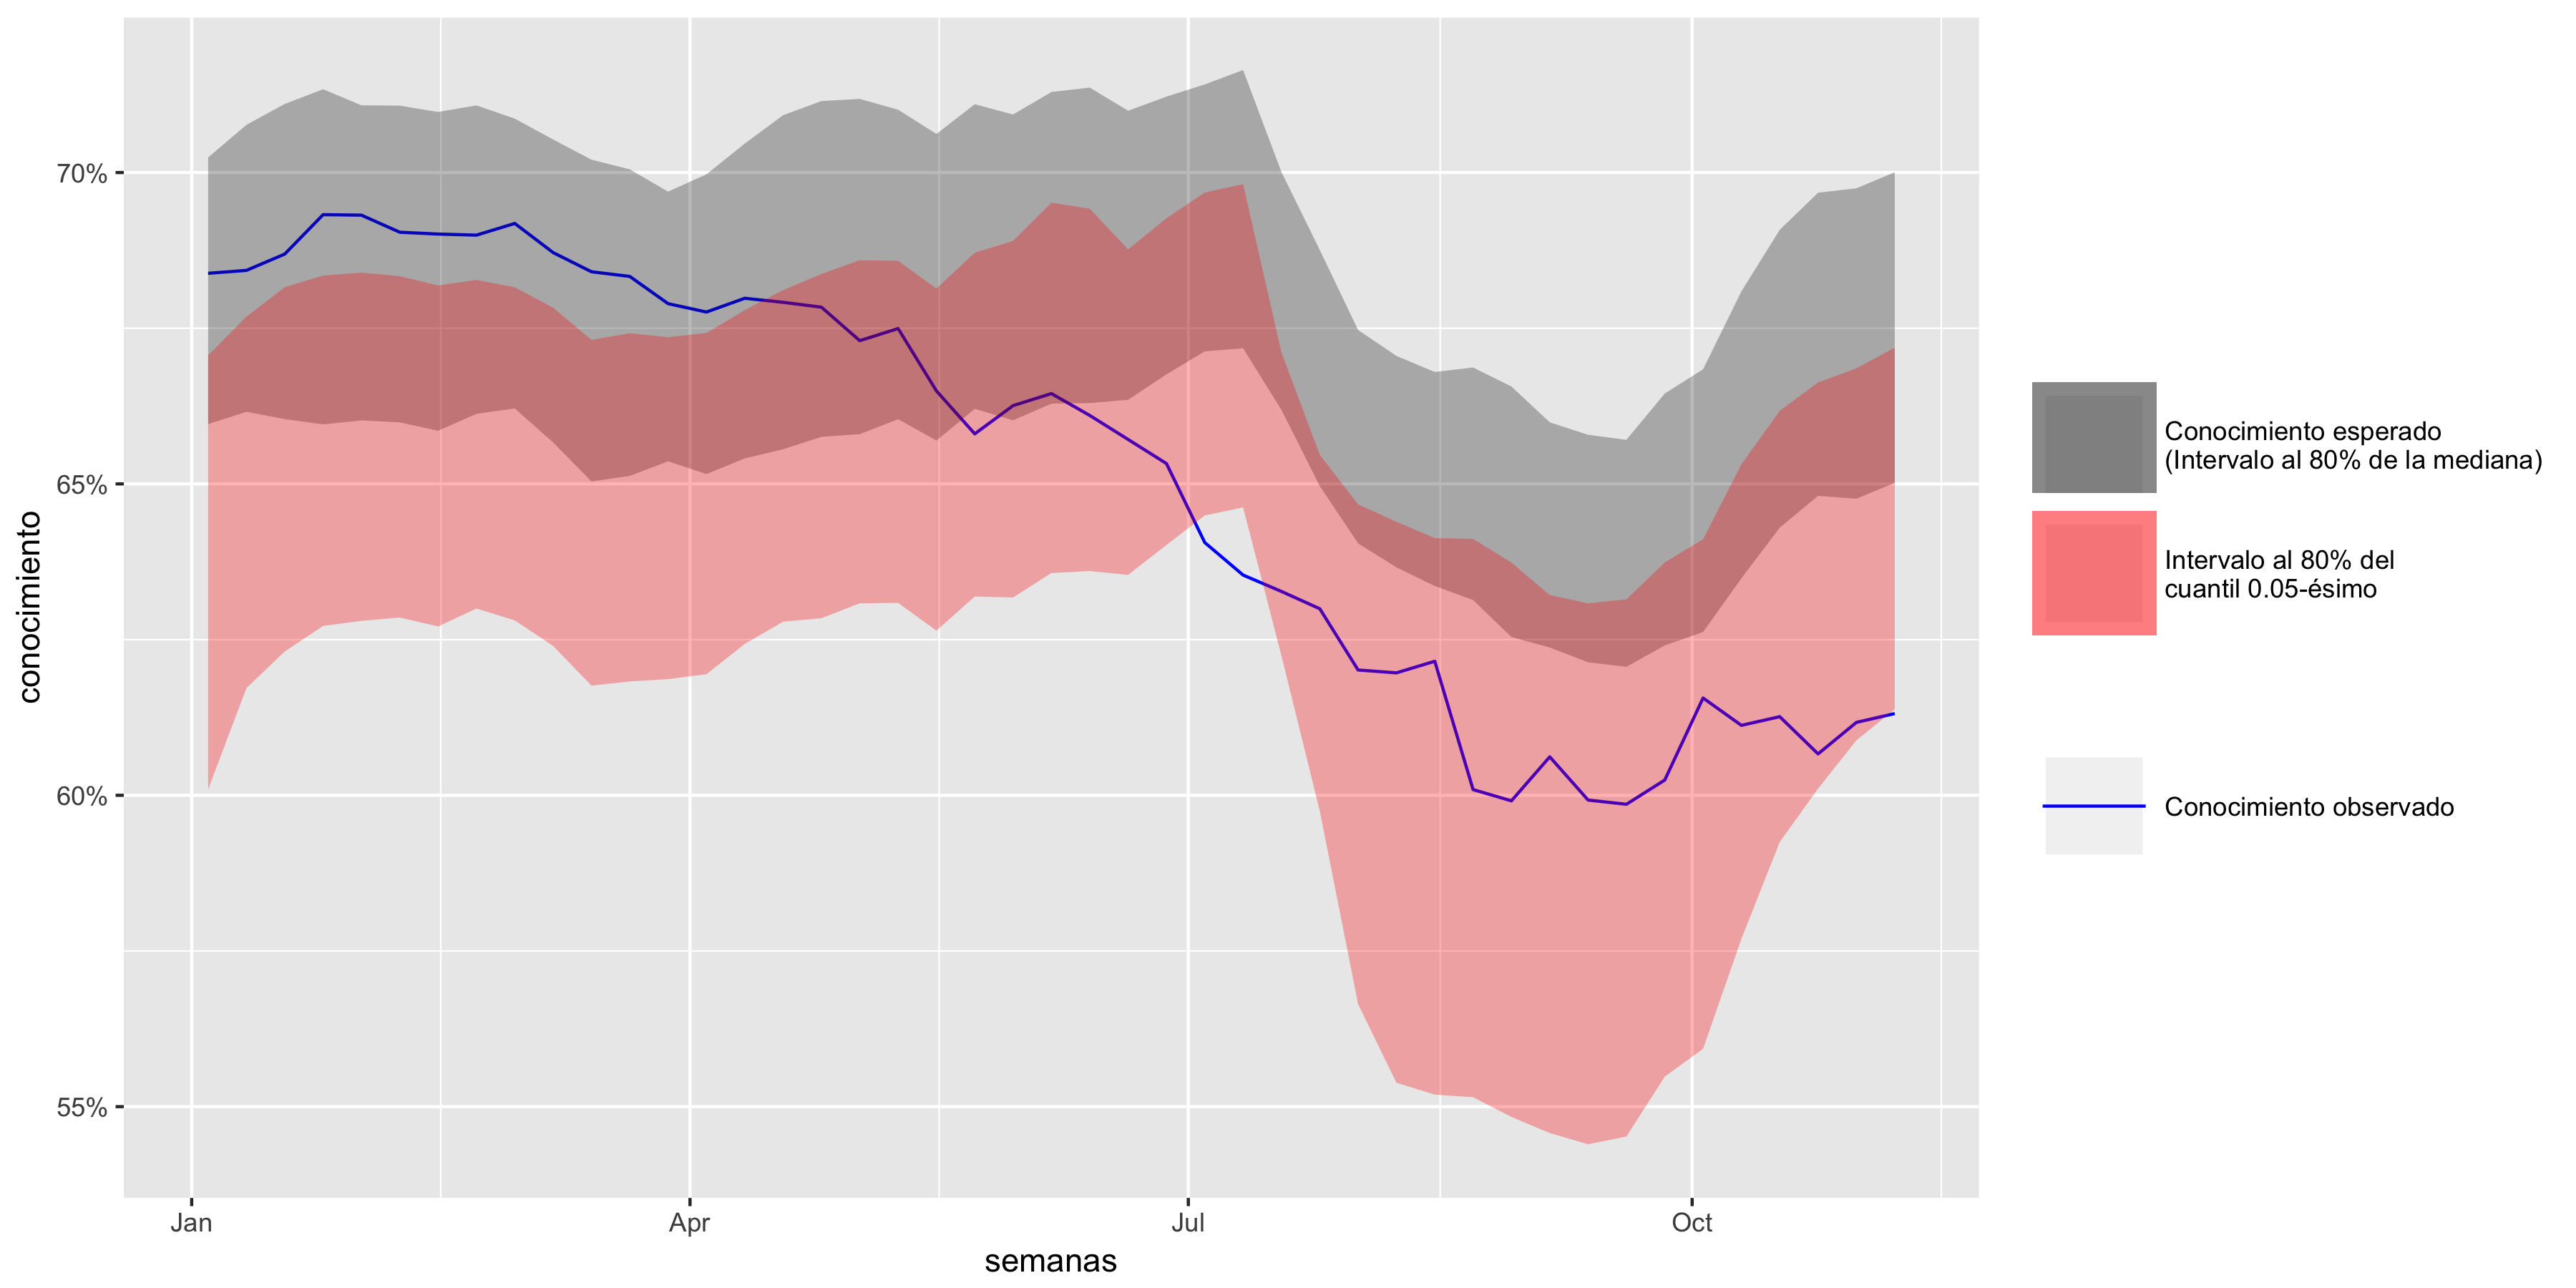
\includegraphics[width=1\textwidth]{Figures/MarketResearch/goals_2016.png}
	\captionsetup{singlelinecheck=off,font=footnotesize}
	\label{awareness_fit}
\end{figure}

Como se puede observar, hasta el mes de abril el \textit{Conocimiento de marca} se comport\'o de acuerdo a lo esperado, pero despu\'es tuvo una ca\'ida estrepitosa que, si bien el modelo hab\'ia anticipado para despu\'es de julio, coincidi\'o en mayor medida con lo que se hubiera esperado para el cuantil $0.05$-\'esimo. Es decir, suponiendo que no hubiera cambio estructural, se habr\'ia presenciado el peor de cada 20 casos.

En otras palabras, confiando en la construcci\'on del modelo, el supuesto de independencia entre las observaciones y un error modesto en la medici\'on del \textit{Conocimiento de marca}, hay informaci\'on suficiente para pensar que, en efecto, el cambio de concepto en los comerciales del competidor impact\'o la m\'etrica del cliente.


\newpage

\chapter[Conclusiones y trabajo futuro]{Conclusiones y trabajo futuro}

Si bien los modelos de regresi\'on a la media han sido de mucha utilidad en las \'ultimas d\'ecadas, principalmente cuando el poder computacional era menor, es importante recalcar que actualmente existen contextos en los que resultan insuficientes, tanto porque se quiere estudiar que tan factible es un valor at\'ipico, o porque se necesita modelar alg\'un fen\'omeno asim\'etrico, por mencionar algunos ejemplos.

De manera similar, la aproximaci\'on lineal y la distribuci\'on Normal del error han sido fundamentales para que los modelos de regresi\'on hayan proliferado en una gran cantidad de industrias, tanto por su interpretabilidad, como por su bajo costo. Pero es imposible ignorar que \'unicamente representan un pequeño subconjunto del universo infinito de funciones y distribuciones posibles. Crear modelos que permitan una mayor flexibilidad acercar\'a m\'as a la Estad\'istica a una representaci\'on certera de la realidad.

Asimismo, utilizar el paradigma bayesiano para realizar este tipo de modelado tiene la ventaja de poder introducir informaci\'on de las y los expertos en el fen\'omeno a estudiar, as\'i como ponderar cu\'ando fiarse m\'as de los datos y cu\'ando de dicho conocimiento. Adem\'as de su construcci\'on axiom\'atica, que todo aquel que disfrute de la formalidad en las Matem\'aticas, valorar\'a.

Si bien estos avances son significativos, a\'un existe mucho que explorar respecto a lo planteado en este trabajo. Por ejemplo, la descomposici\'on de la funci\'on aproximada del cuantil en muchos procesos gaussianos, uno por covariable, dar\'a un mayor peso a aquellas covariables que en efecto sean m\'as significativas para explicar el fen\'omeno en cuesti\'on. 

Por otro lado, la inclusi\'on de un parametro que regule din\'amicamente la relaci\'on entre la distancia y la covarianza entre observaciones, de acuerdo al fen\'omeno y a las covariables usadas, brindar\'a mayor flexibilidad, y por ende, mejor ajuste al modelo.

\newpage 

%%%%%%%%%%%%%%%%%%%%%%%%%%%%%%%%%%%%%%%%%%%%%%%%%%%%%%%%%%%%%
%%    Bibliografia
%%%%%%%%%%%%%%%%%%%%%%%%%%%%%%%%%%%%%%%%%%%%%%%%%%%%%%%%%%%%%
\nocite{*} %Even non-cited BibTeX-Entries will be shown.
\bibliographystyle{authordate1} %Style of Bibliography: plain / apalike / amsalpha / ...
\bibliography{Bibliography} %You need a file 'literature.bib' for this.

%%%%%%%%%%%%%%%%%%%%%%%%%%%%%%%%%%%%%%%%%%%%%%%%%%%%%%%%%%%%%
%%  Apendices
%%%%%%%%%%%%%%%%%%%%%%%%%%%%%%%%%%%%%%%%%%%%%%%%%%%%%%%%%%%%%
\appendix

\chapter[Algoritmos MCMC]{Algoritmos MCMC\footnote{Las ideas de este ap\'endice son retomadas de \cite{Robert_MCMC}} }\label{chap:MCMC}

\section {Introducci\'on}

Los algoritmos MCMC son utilizados para aproximar distribuciones de probabilidad, normalmente complejas. La idea es lograr simular una muestra de la distribuci\'on, para poder aproximar sus caracter\'isticas. Entre m\'as grande sea la muestra, mejor ser\'a la estimaci\'on.

Para hacer esto simula cadenas de markov de los distintos elementos de la distribuci\'on compleja, y, bajo el supuesto de que se alcanza la distribuci\'on estacionaria, toma al conjunto de dichas esas simulaciones como una muestra de la distribuci\'on original. De hecho, el nombre MCMC viene del ingl\'es \textit{Monte Carlo Markov Chains}, haciendo tambi\'en referencia a la simulaci\'on de Monte Carlo para cada iteraci\'on.

\section{Simulador de Gibbs}

Se trata de un caso particular de los algoritmos \textit{MCMC}, y a continuaci\'on se analizan dos tipos, siendo el segundo una generalizaci\'on del primero.

\subsection{Simulador de Gibbs de dos pasos}

Funciona de la siguiente manera: si dos variables aleatorias $X$ y $Y$ tienen una densidad conjunta $f(x,y)$, con sus correspondientes densidades condicionales $f_{Y|X}$ y $f_{X|Y}$, se genera una cadena de markov $(X_t,Y_t)$ de acuerdo al siguiente algoritmo:
\\ \\
\begin{algorithm}[H]
 {Tomar $X_0 = x_0$ arbitraria \;
     \For{$t=1,2,...,n$}
     {
        $1. \text{ } Y_t \sim f_{Y|X}(y|x_{t-1})\;$\\
        $2. \text{ } X_t \sim f_{X|Y}(x|y_{t})\;$
     }
 }
 \caption{Simulador de Gibbs de dos pasos}
\end{algorithm}
\BlankLine

La convergencia de la cadena de markov está asegurada, a menos que los soportes de las condicionales no estén conectados.

\subsection{Simulador de Gibbs de múltiples pasos}

Sea $\mathbb{X} \in \mathcal{X}$ una variable aleatoria que puede ser escrita como $\mathbb{X} = (X_1,...,X_p)$, con $p \in \mathbb{Z}^+$, y donde las $X_i$'s bien pueden ser unidimensionales o multidimensionales. Además, es posible encontrar las distribuciones condicionales, de forma que
\begin{equation*}
\begin{aligned}
X_i|x_1,...,x_{i-1},x_{i+1},...,x_p &\sim f_i(x_i|x_1,...,x_{i-1},x_{i+1},...,x_p) \text{, }\\
i &\in \{1,...,p\}.
\end{aligned}
\end{equation*}

El correspondiente algoritmo de Gibbs está dado por:
\\ \\
\begin{algorithm}[H]
 Tomar $\textbf{x}^{(0)} = (x_1^{(0)},...,x_p^{(0)})$ arbitraria\;
 \For{$t=1,2,...,n$}
 {
    $1. \text{ } X_1^{(t)} \sim f_1(x_1|x_2^{(t-1)},...,x_p^{(t-1)})\;$\\
    $2. \text{ } X_2^{(t)} \sim f_2(x_2|x_1^{(t)},x_3^{(t-1)},...,x_p^{(t-1)})\;$\\
    $...\;$\\
    $k.  \text{ } X_k^{(t)} \sim f_k(x_k|x_1^{(t)},...,x_{k-1}^{(t)},x_{k+1}^{(t-1)},...,x_p^{(t-1)})\;$\\
    $...\;$\\
    $p.  \text{ }X_p^{(t)} \sim f_p(x_p|x_1^{(t)},...,x_{p-1}^{(t)})\;$\\
 }
 \caption{Simulador de Gibbs de múltiples pasos}
\end{algorithm}
\BlankLine

Cabe resaltar que el desempeño puede estar fuertemente afectado por la parametrización del modelo. Por ello puede resultar una buena idea reparametrizar el modelo, buscando que las componentes sean lo más independientes posible.

\section {Monitoreo de convergencia y adaptación de los algortimos MCMC}

\subsection{Monitoreo de convergencia a la \textit{estacionariedad}}

El primer requisito de convergencia de un algoritmo MCMC es que la distribución de la cadena $(x^{(t)})$ sea la distribución estacionaria $f$. Una meta menos ambiciosa sería que sea independiente del punto inicial $x^{(0)}$, después de muchas realizaciones de la cadena. La principal herramienta para verificar \textit{estacionariedad} es correr varias cadenas en paralelo, para poder comparar sus rendimientos. 

Un primer acercamiento empírico al control de convergencia es el dibujar gráficas de las cadenas simuladas (componente a componente o juntas), para detectar valores muy desviados y comportamientos no estacionarios. 

Otro diagnóstico gráfico que se puede utilizar es la \textit{traza}, es decir, la gr\'afica de cada uno de los valores de la cadena en el eje $y$, contra su respectivo n\'umero de iteraci\'on en el eje $x$. As\'i ser\'a posible observar cuando la cadena tiene un comportamiento repetitivo en ciertos valores y a partir de qu\'e momento se distribuye sobre todo el soporte, es decir, a partir de qu\'e iteraci\'on alcanza la distribuci\'on estacionaria. 

\subsection{Monitoreo de convergencia a los promedios}

Una vez cubierta la distribución estacionaria, se verifica la convergencia del promedio aritmético
\begin{equation*}
    \frac{1}{T}\sum_{t=1}^T h(x^{(t)})
\end{equation*}
a la esperanza $\mathbb{E}_f[h(x)]$, para una función $h$ arbitraria. Esto propiedad se denomina com\'unmente \textit{ergodicidad}.

La herramienta inicial y más natural suele ser el graficar la evolución del estimador del promedio, conforme crece $T$. Si dicha curva no se ha estabilizado después de $T$ iteraciones, habría que incrementar la longitud de la cadena de markov.

\subsection{Monitoreo de convergencia a una muestra \textit{iid}}

Para finalizar, idealmente, la aproximación de $f$ obtenida de los algortimos MCMC se debería extender a la producción (aproximada) de muestras $iid$ de $f$. La técnica más usada para lograr esto es el \textit{submuestreo o refinamiento}, donde se consideran s\'olo los valores $y^{(t)} = x^{(kt)}$, para cierta $k$.

Como medidas diagn\'ostico normalmente se usan las siguientes: la autocorrelaci\'on dentro de cada variable aleatoria que es parte del simulador de Gibbs; y la correlaci\'on cruzada entre las distintas variables aleatorias, dado que se busca independencia entre ellas.

\newpage


\end{document}

